% !TeX root = ../main.tex

\chapter{Numerical Results}

Within this chapter, we conduct several numerical tests to appraise the error coNumerical Resultnvergence speed and computational efficiency of our polynomial option pricing method. The implementation is uncomplicated. Our focus is primarily on various polynomial options, along with call options and polynomial options, and an analysis of various processes for price dynamics. 

All experiments are performed under the parameters setting shown in the following related to the specified stochastic processes.
\begin{itemize}
    \item Common parameters: 
    $$r = 0.05, \quad T = 0.5, \quad \sigma = 0.2.$$
    \item Stochastic volatility parameters: 
    $$\kappa_v = 3, \quad \overline{\nu} = 0.04, \quad \sigma_v=0.1 \quad \rho = -0.1.$$
    \item Jump process parameters: 
    $$\lambda = 140, \quad \gamma = 0.01, \quad \delta = 0.02.$$
    \item Double exponential Jump parameters:
    $$\lambda_e = 1, \quad p = 0.4, \quad \eta_1 = 10, \quad \eta_2 = 5.$$  
    \item Normal inverse Gaussian related parameters:
    $$\alpha = 1.326, \quad \beta = 15.624, \quad \xi = 4.025.$$
    \item Variance gamma parameters:
    $$\theta = -0.14, \quad \omega = 0.2.$$
\end{itemize}

When performing the following calculations, it is necessary to consider how to choose the truncation range of the improper integral which is $\left[l, \, u\right]$. The probability density function can be expressed by 
\begin{align}
    f\left(x\right) &\approx \sum_{k=0}^{\infty}^{'} F_k \mathrm{cos}\left(k\pi \frac{x-l}{u-l}\right) \nonumber \\
    &\approx \sum_{k=0}^{N-1}^{'} F_k \mathrm{cos}\left(k\pi \frac{x-l}{u-l}\right), \label{density_ft}
\end{align}
where 
\begin{align*}
F_k = \frac{2}{u-l}\mathrm{Re}\left\{ \phi\left(\frac{k\pi}{u-l}\right) \mathrm{exp}\left(-i\frac{kl\pi}{u-l}\right) \right\}.
\end{align*}

My approach is to first operate over a relatively large price range, in this study $\left[10^{-15}, \,10^{20}\right]$, to simulate the pre-trained probability distribution with a large value of $N$, in this study $10^5$, as a true probability proxy based on (\ref{density_ft}). Based on this density proxy, I first developed a program to search both sides for the point where the density value is less than a predetermined threshold, in this study $10^{-6}$, so we get the first pair of endpoints. Then, I identify other pairs of endpoints where the product of the payoff function and the probability density is below a given acceptable error. Among two pairs of endpoints, we determine the smallest one as $l$ and the largest one as $u$. The reason why we need to first find only in the density function is that we need full information to simulate the density function. The value product of the density and payoff function will become zero when the payoff function is zero where the range does not fit the whole density. The reason why we can always find $l$, $u$ is that all price dynamics distributions decrease exponentially on both sides, which overwhelms any polynomial growth rate. Therefore, we can find two endpoints where the option value is less than the given acceptable error outside of these two endpoints. In other words, we look for the points outside of which the values of the option can be ignored, and these points become the upper and lower bounds of the truncation range of my model.

Note that for the Monte-Carlo simulation experiments conducted in this thesis, all confidence intervals in the following experiments are within two standard-error.
\section{Call Options}
In this section, we focus on call options. While there are already many efficient methods for pricing call options, my pricing model is designed to efficiently price not only call options but also other types of options by simply adjusting the input of the coefficients of the payoff function as a polynomial function. This section aims to demonstrate the flexibility of this model. That is you only need to write the program once, and you can price every option whose payoff function is a subset of the polynomial option without any adjustment. In other words, my model can be used to price call options without any modifications, even though it is capable of pricing a wide range of options efficiently. 

All the experiments in this section are under the same configuration which is $S_0=100$, $K=100$, and the payoff function is $(S_T - 100)^+$. In my model setting, it's necessary to separate the payoff function into two parts which are an array of polynomial coefficients and an array of positive intervals as inputs. Positive intervals refer to an interval in which the stock prices within the interval will not cause the payoff function to be less than zero. Based on the mathematical property of the polynomial function, this interval corresponds to all positive real roots. As a result, the array of polynomial coefficients is $\left[ -100, \,1\right]$, and the array of the positive interval is $\left[100, \, \infty\right]$.

Note that the reference values for analyzing error convergence are calculated using an analytic solution only for geometric Brownian motion, stochastic volatility model, and log-normal jump diffusion. For other stochastic processes, these reference values are calculated under my model with $N=10^5$. These values fall within the confidence interval constructed by simulating $10^7$ paths with a two-standard-error width.
\newpage

\subsection{Geometric Brownian Motion}
\begin{figure}[H]
    \centering
    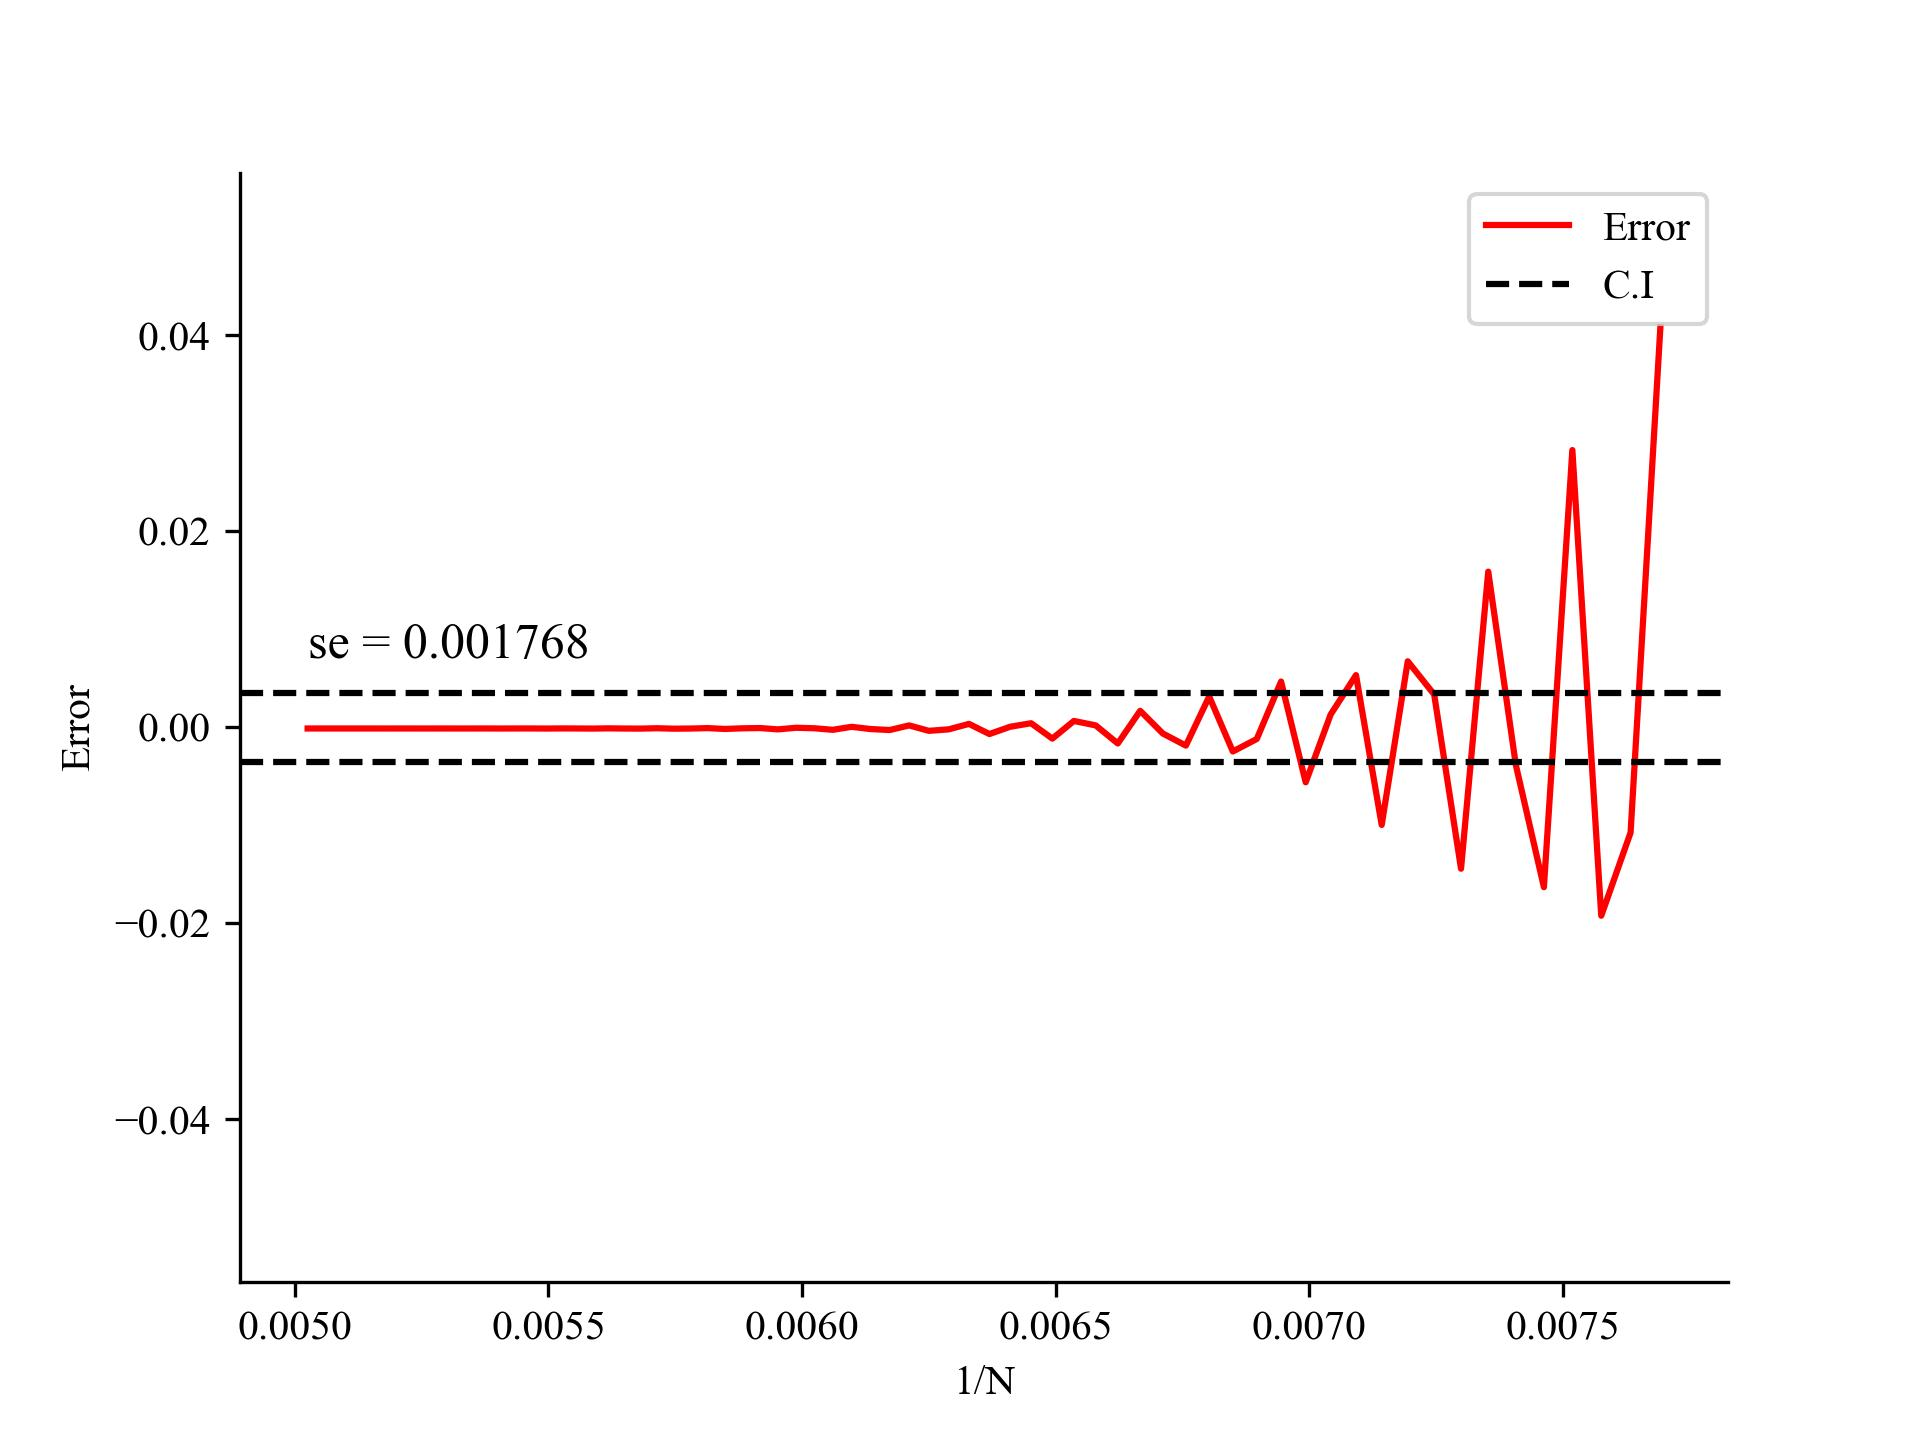
\includegraphics[width=0.8\linewidth]{value-plot-GBM-call.jpg}
    \caption[\emph{GBM-Call: Value accuracy comparing to the simulation with} $10^7$ \emph{paths.} ] {\emph{GBM-Call: Value accuracy comparing to the simulation with} $10^7$ \emph{paths.} \textbf{Note}: mean value from simulation = 6.885240, criteria of negligible error from the product of payoff function and density is $10^{-6}$, and $N$ starts from $10$ with increment $=2$.}

    \label{fig:label}
\end{figure}

\begin{figure}[H]
    \centering
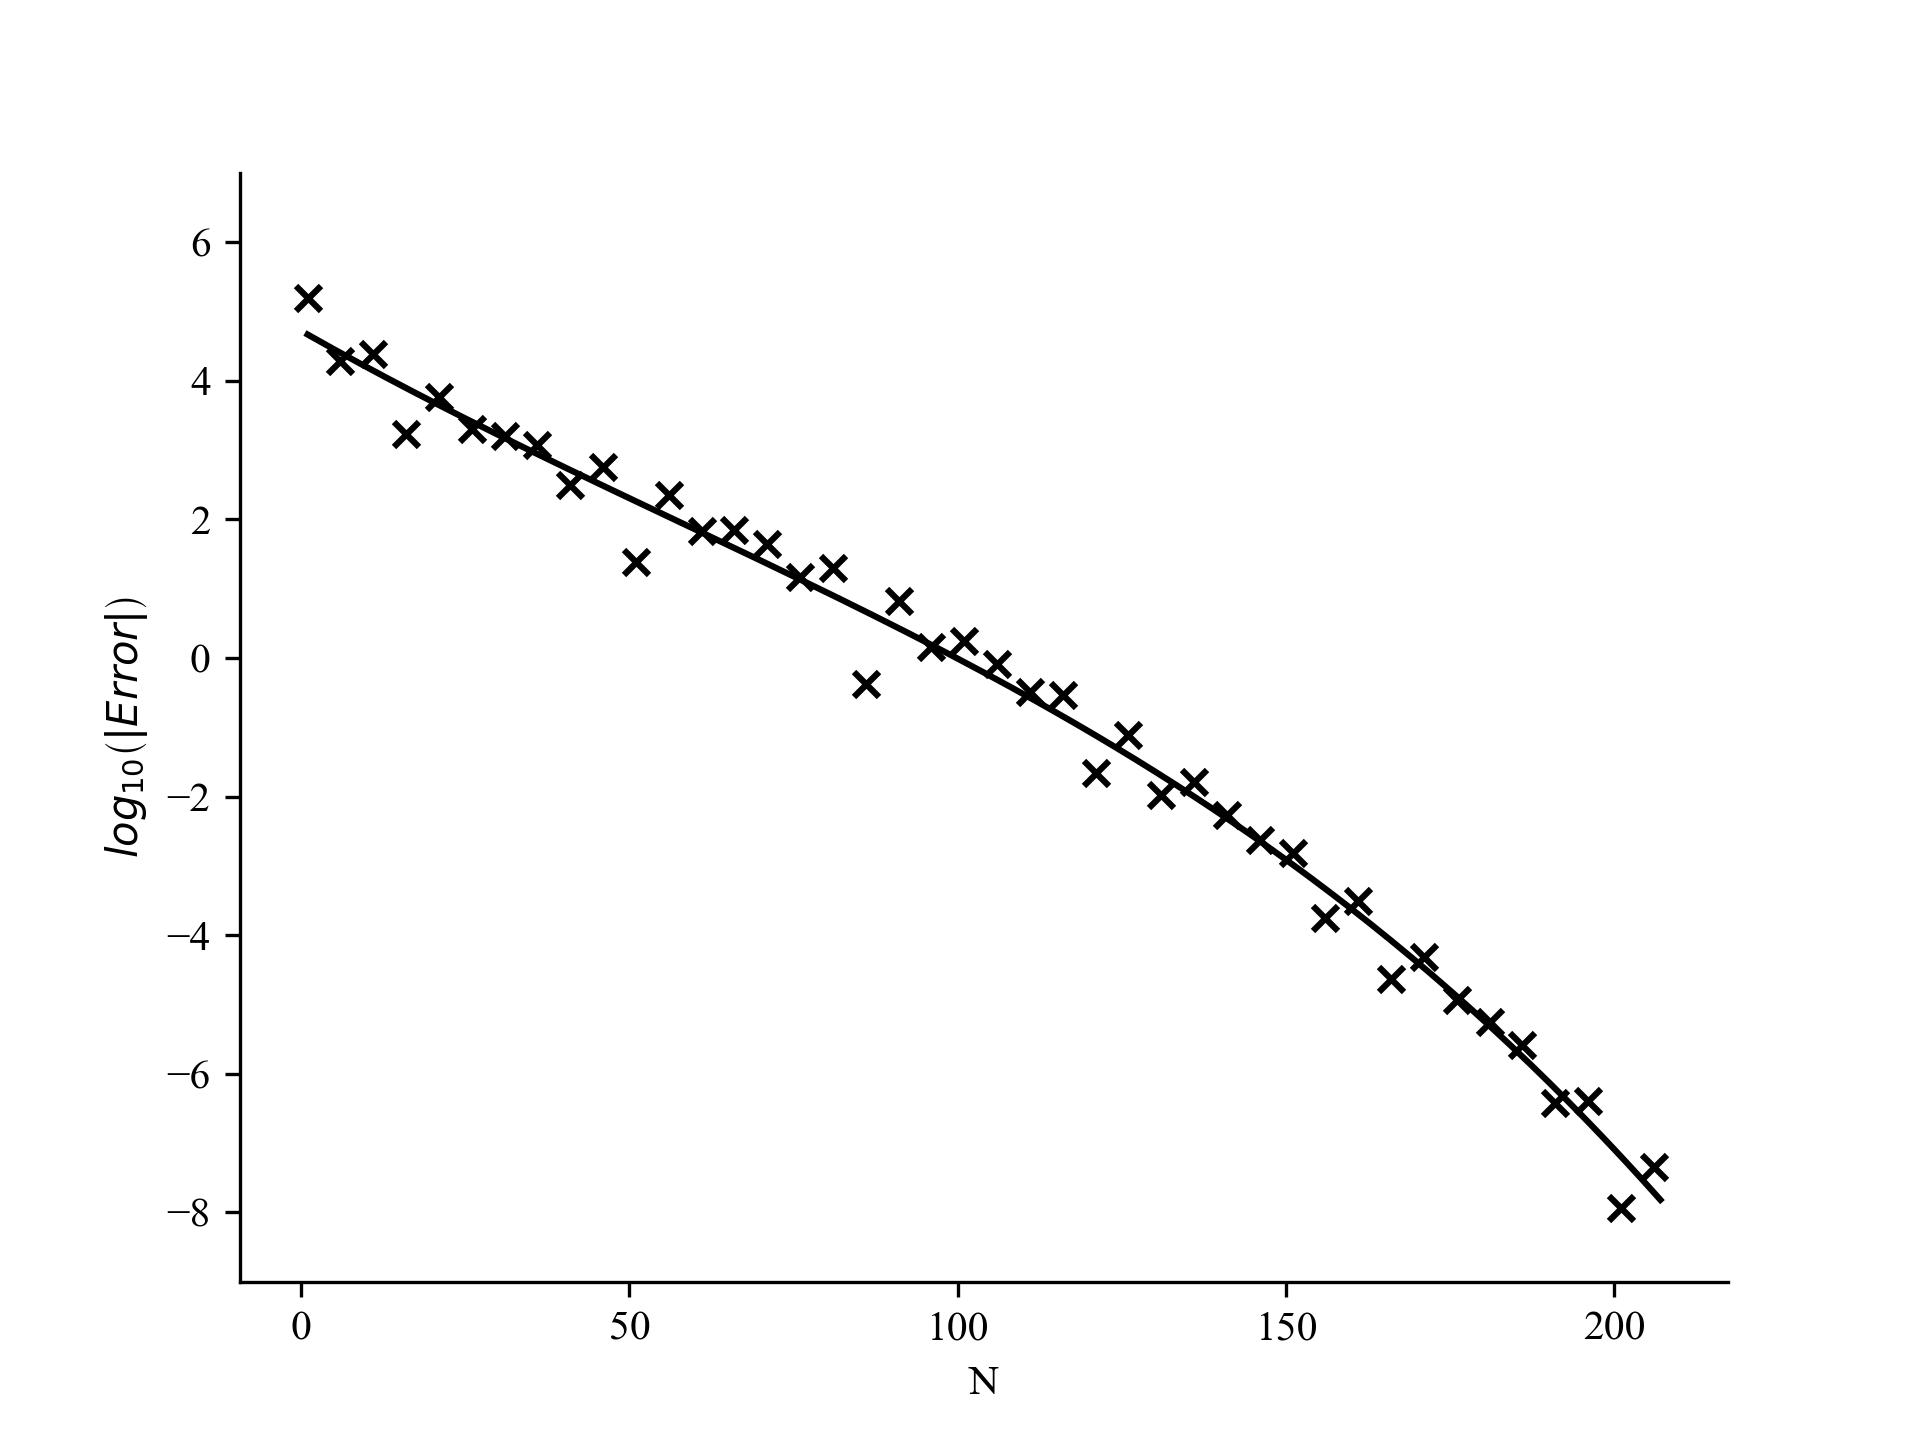
\includegraphics[width=0.8\linewidth]{error-plot-GBM-call.jpg}
    \caption[GBM-Call: \emph{The speed of error convergence.} ]{GBM-Call: \emph{The speed of error convergence.} \textbf{Note}: reference value $=6.8887285777$, criteria of negligible error from the product of payoff function and density is $10^{-15}$, $R^2=0.990$, and the regression line is $log_{10}\left(|Error|\right) = 0.0002N^2-0.0539N+4.7202$.}
    
    \label{fig:label}
\end{figure}

\subsection{Stochastic Volatility Model}
\begin{figure}[H]
    \centering
    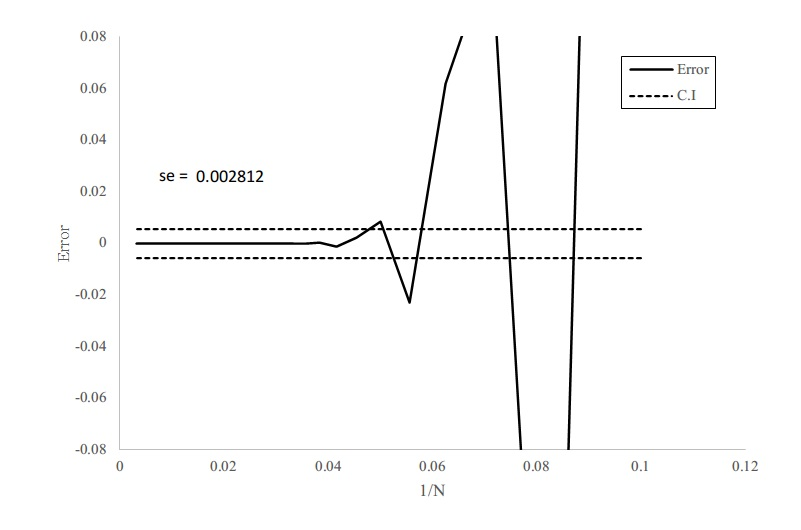
\includegraphics[width=0.8\linewidth]{value-plot-Heston-call.jpg}
    \caption[\emph{SV-Call: Value accuracy comparing to the simulation with} $10^7$ \emph{paths.}]{\emph{SV-Call: Value accuracy comparing to the simulation with} $10^7$ \emph{paths.} \textbf{Note}: mean value from simulation = 6.881753, criteria of negligible error from the product of payoff function and density is $10^{-6}$, and $N$ starts from $10$  with increment $=2$.}
    
    \label{fig:label}
\end{figure}

\begin{figure}[H]
    \centering
    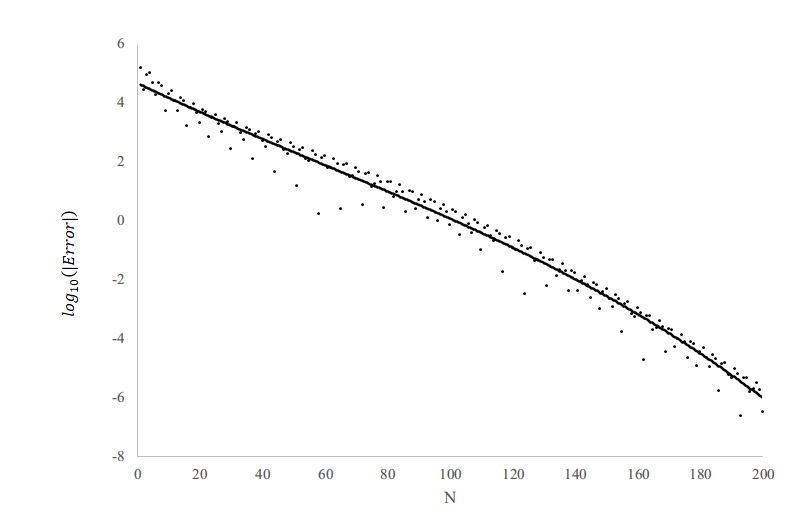
\includegraphics[width=0.8\linewidth]{error-plot-Heston-call.jpg}
    \caption[\emph{SV-Call: The speed of error convergence.}]{\emph{SV-Call: The speed of error convergence.} \textbf{Note}: reference value $=6.8816576853$, criteria of negligible error from the product of payoff function and density is $10^{-15}$, $R^2=0.989$, and the regression line is $log_{10}\left(|Error|\right) = 7.26\times 10^{-5}N^2-0.0482N+4.6371$.}
    \label{fig:label}
\end{figure}




\subsection{Log-normal Jump Diffusion Model}
\begin{figure}[H]
    \centering
    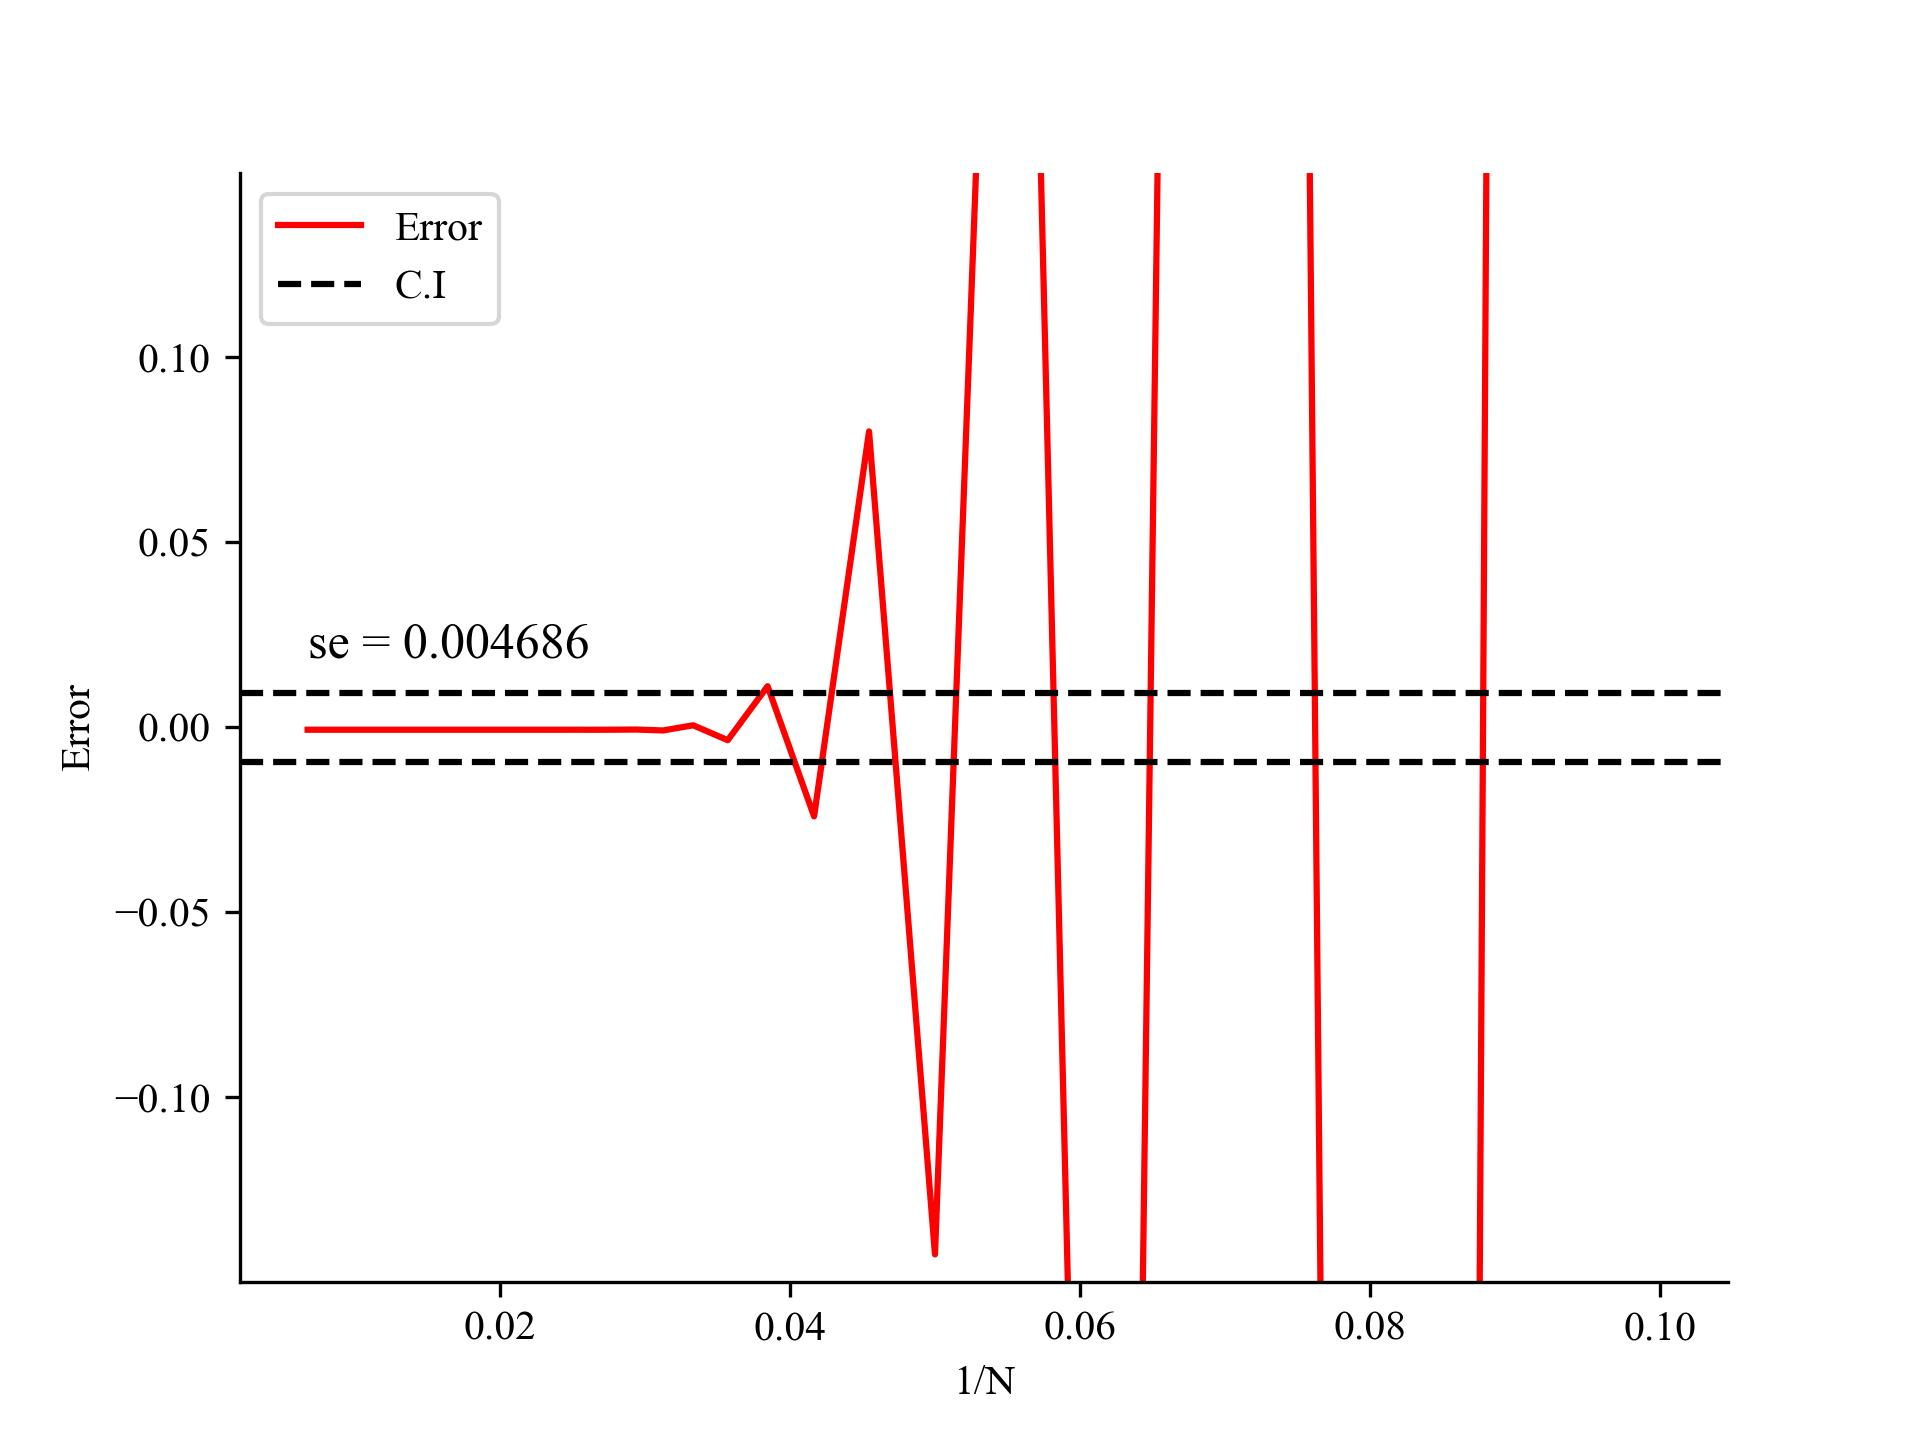
\includegraphics[width=0.8\linewidth]{value-plot-MJD-call.jpg}
    \caption[\emph{JD-Call: Value accuracy comparing to the simulation with}]{\emph{JD-Call: Value accuracy comparing to the simulation with} $10^7$ \emph{paths.} \textbf{Note}: mean value from simulation = 10.528850, criteria of negligible error from the product of payoff function and density is $10^{-6}$, and $N$ starts from $10$  with increment $=2$.}
    
    \label{fig:label}
\end{figure}

\begin{figure}[H]
    \centering
    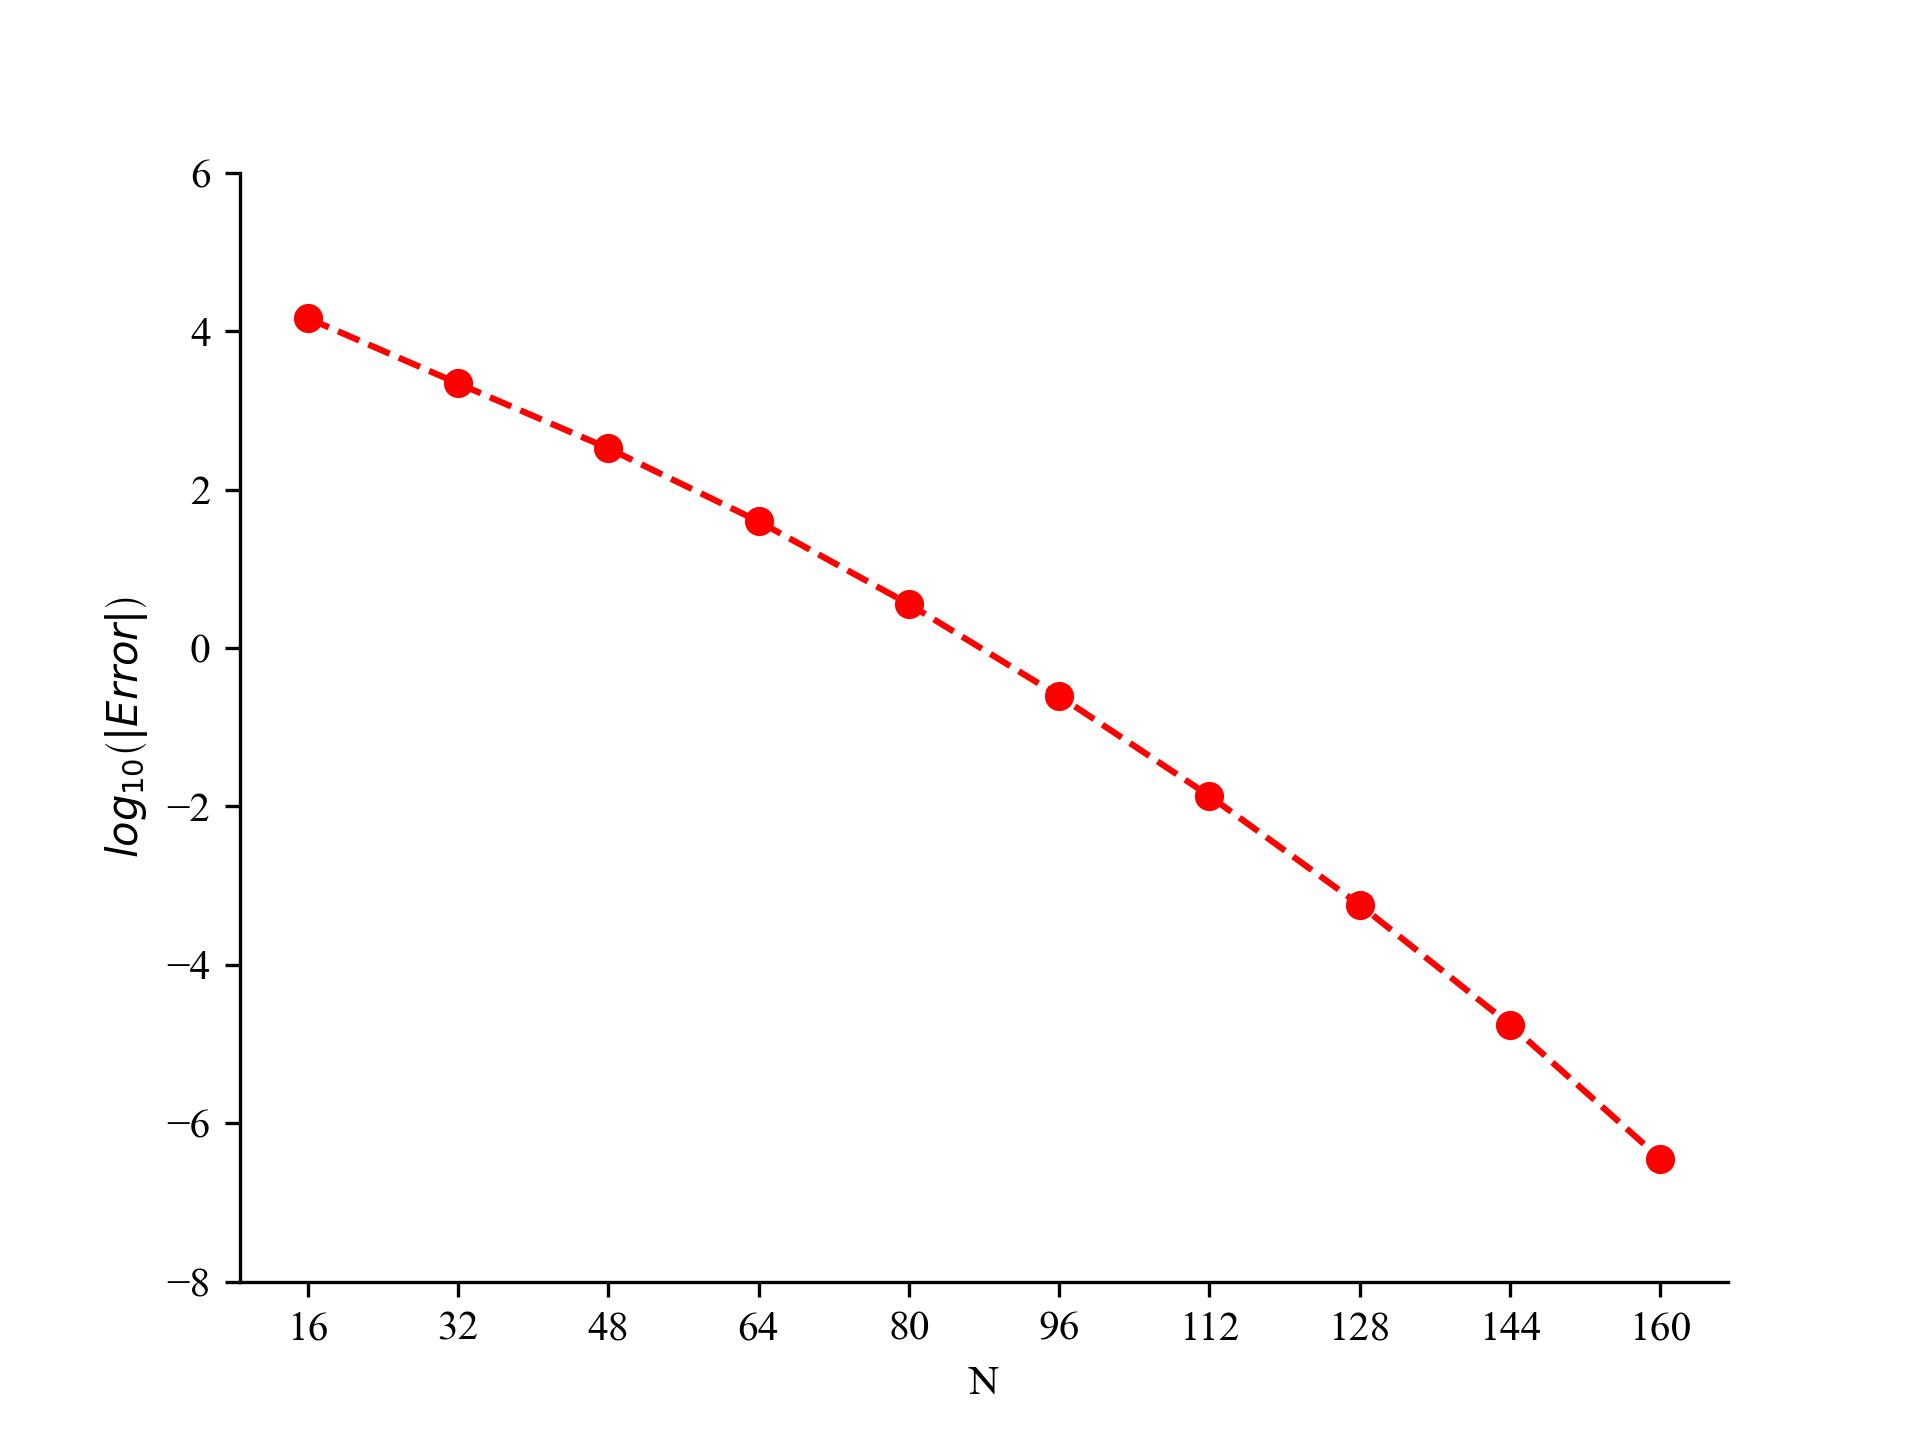
\includegraphics[width=0.8\linewidth]{error-plot-MJD-call.jpg}
    \caption[\emph{JD-Call: The speed of error convergence.}]{\emph{JD-Call: The speed of error convergence.} \textbf{Note}: reference value $=10.5281599666$, criteria of negligible error from the product of payoff function and density is $10^{-15}$, $R^2=0.994$, and the regression line is $log_{10}\left(|Error|\right) = -8.33\times 10^{-6}N^2-0.0448N+5.1472$.}

    \label{fig:label}
\end{figure}



\subsection{Double Exponential Jump Diffusion Model}
\begin{figure}[H]
    \centering
    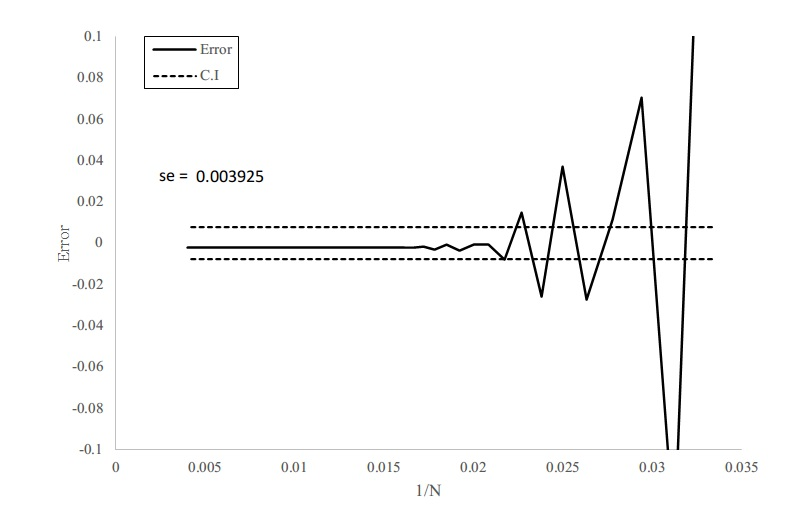
\includegraphics[width=0.8\linewidth]{value-plot-KJD-call.jpg}
    \caption[\emph{DJD-Call: Value accuracy comparing to the simulation with} $10^7$ \emph{paths.}]{\emph{DJD-Call: Value accuracy comparing to the simulation with} $10^7$ \emph{paths.} \textbf{Note}: mean value from simulation = 8.829095, criteria of negligible error from the product of payoff function and density is $10^{-6}$, and $N$ starts from $10$  with increment $=2$.}

    \label{fig:label}
\end{figure}

\begin{figure}[H]
    \centering
    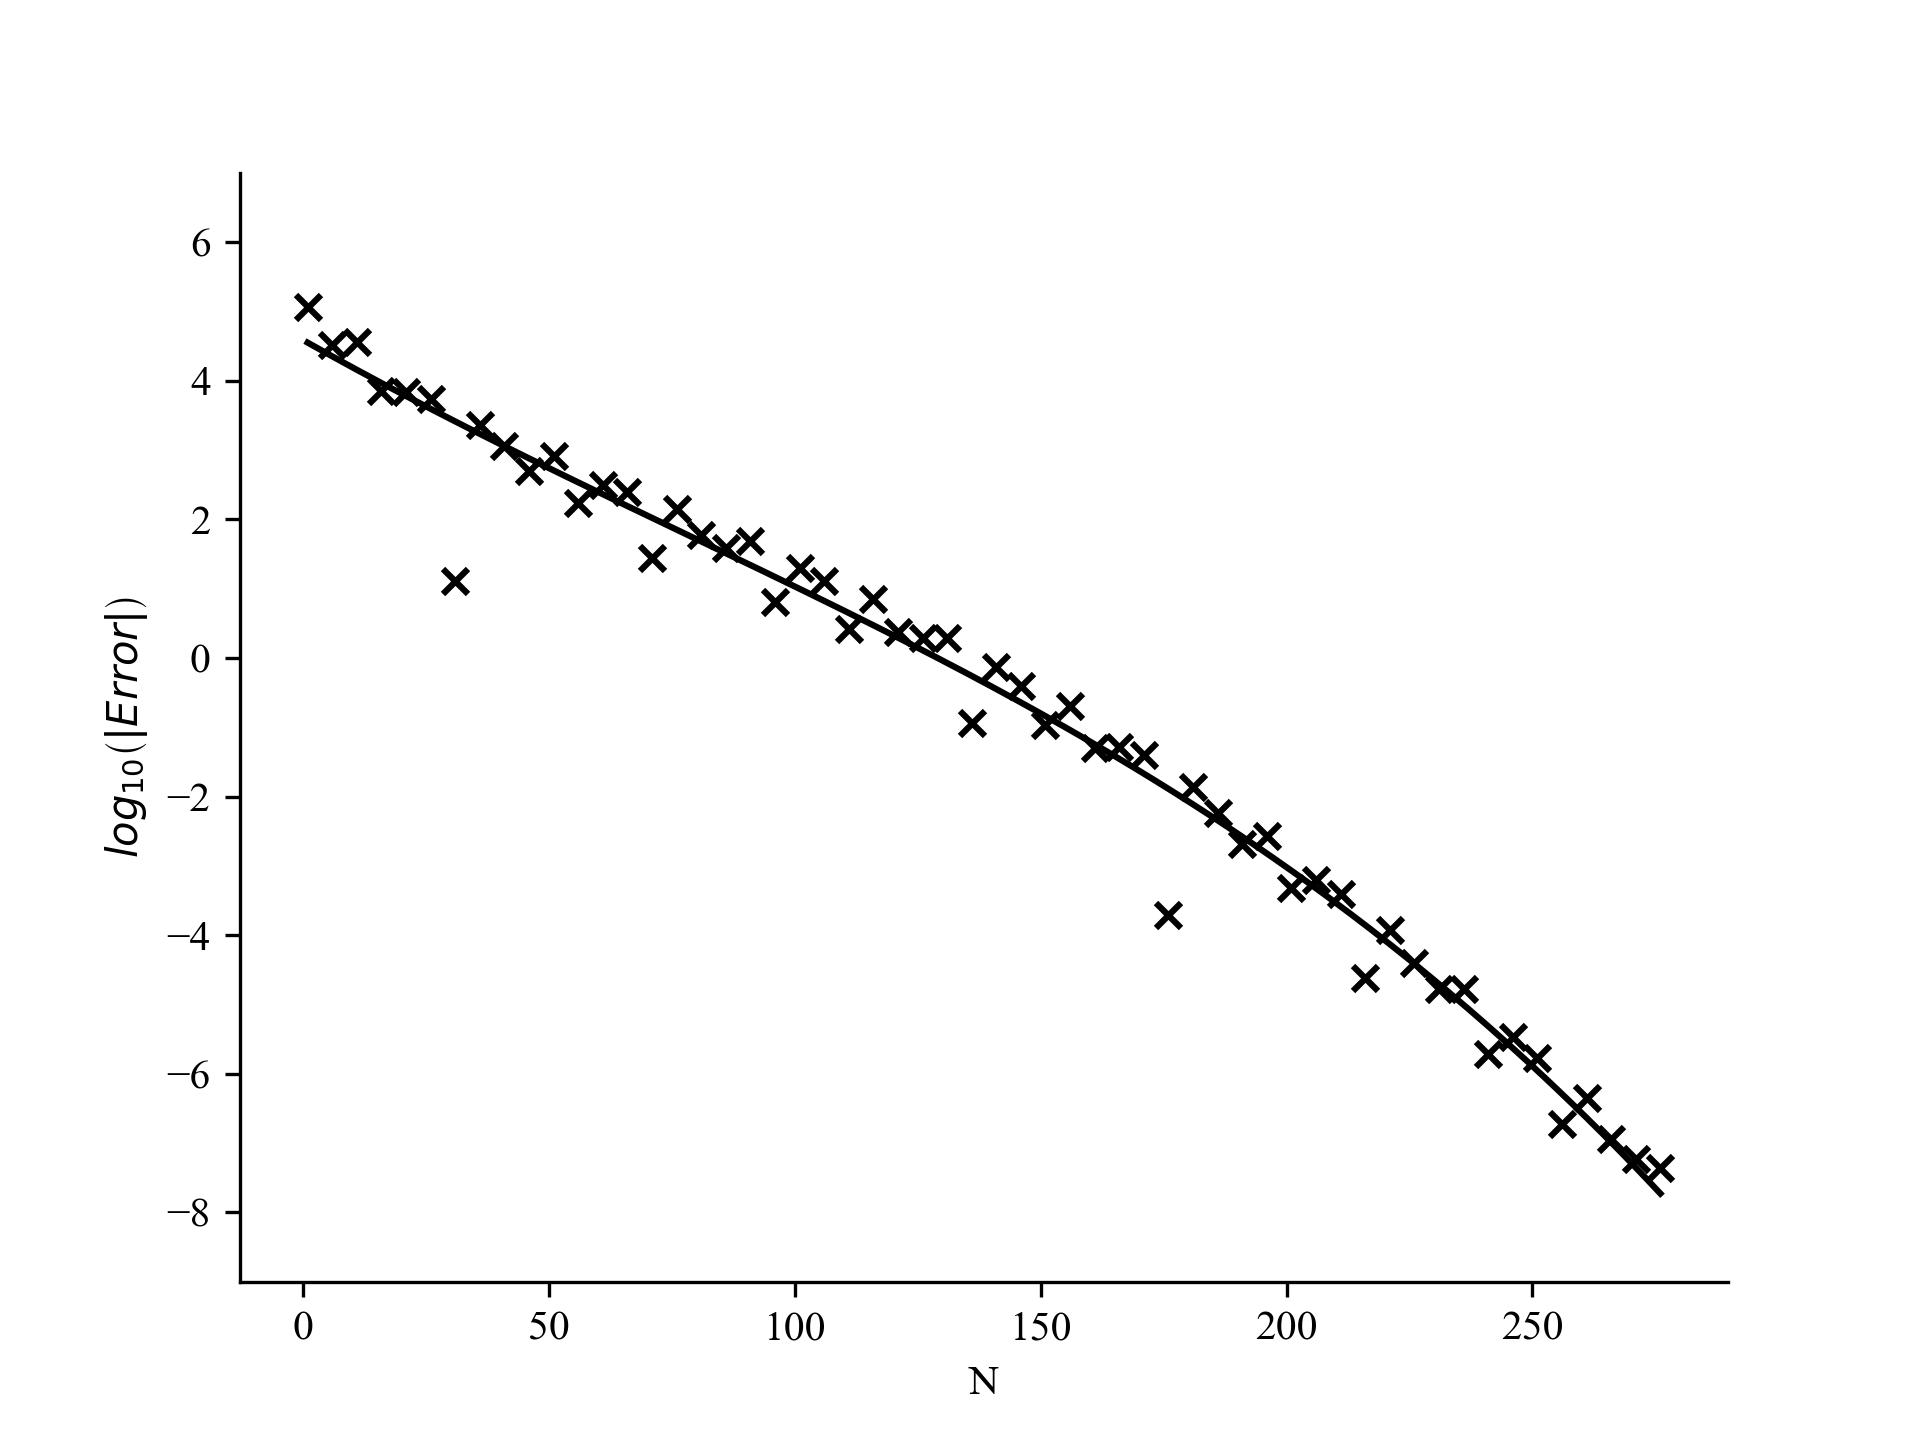
\includegraphics[width=0.8\linewidth]{error-plot-KJD-call.jpg}
    \caption[\emph{DJD-Call: The speed of error convergence.}]{\emph{DJD-Call: The speed of error convergence.} \textbf{Note}: reference value $=8.8270603863$, criteria of negligible error from the product of payoff function and density is $10^{-15}$, $R^2=0.990$, and the regression line is $log_{10}\left(|Error|\right) = -8.097\times 10^{-5}N^2-0.0402N+4.5899$.}
    
    \label{fig:label}
\end{figure}



\subsection{Stochastic Volatility Jump Model}
\begin{figure}[H]
    \centering
    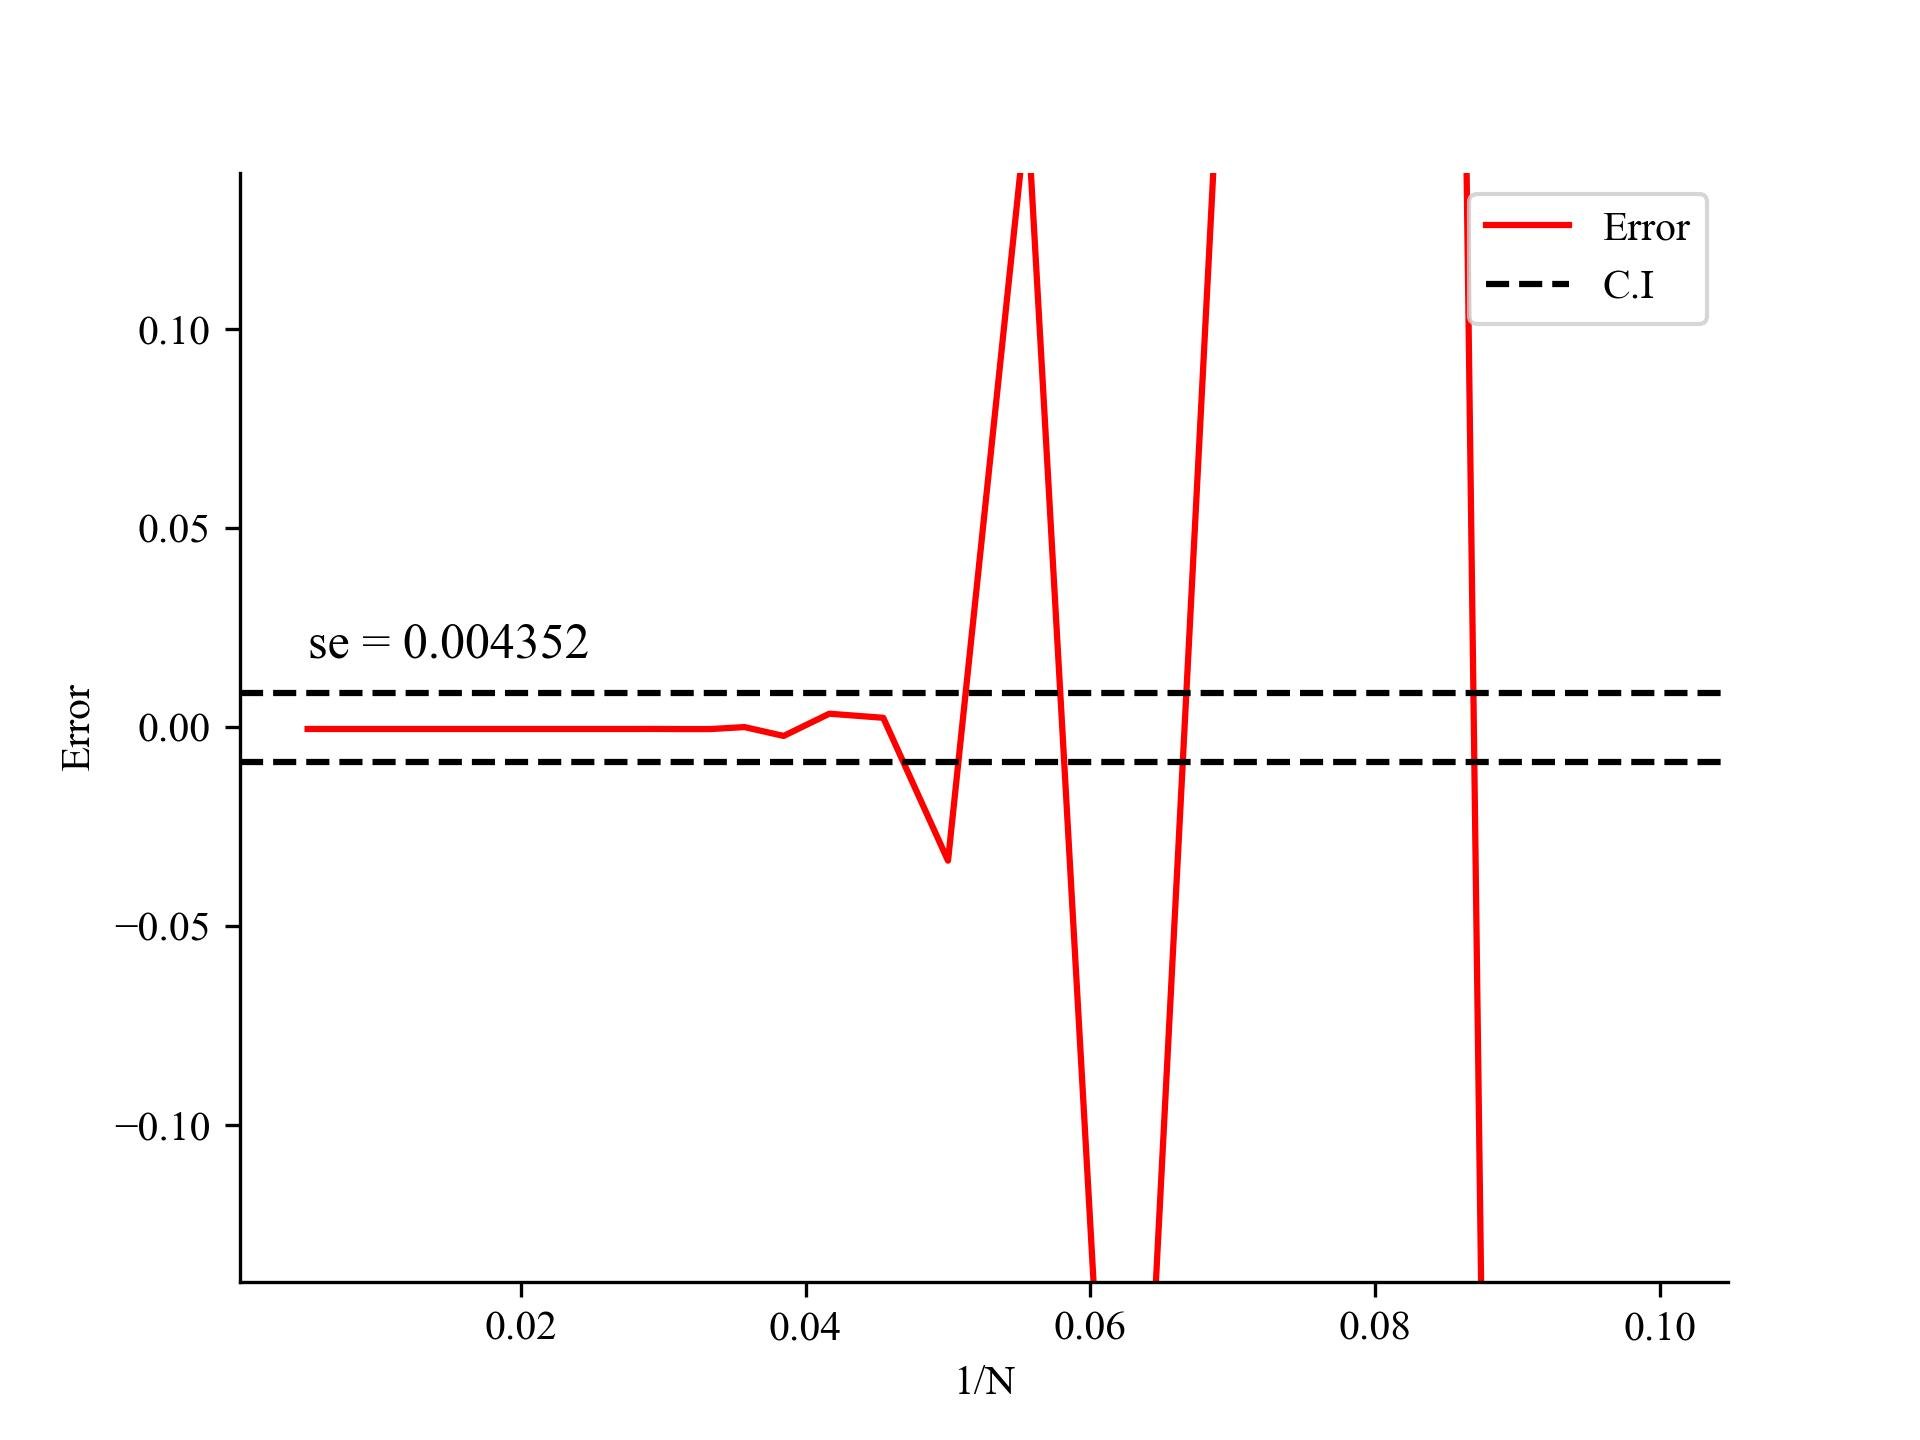
\includegraphics[width=0.8\linewidth]{value-plot-SVJ-call.jpg}
    \caption[\emph{SVJ-Call: Value accuracy comparing to the simulation with} $10^7$ \emph{paths.}]{\emph{SVJ-Call: Value accuracy comparing to the simulation with} $10^7$ \emph{paths.} \textbf{Note}: mean value from simulation = 10.525662, criteria of negligible error from the product of payoff function and density is $10^{-6}$, and $N$ starts from $10$  with increment $=2$.}
    
    \label{fig:label}
\end{figure}

\begin{figure}[H]
    \centering
    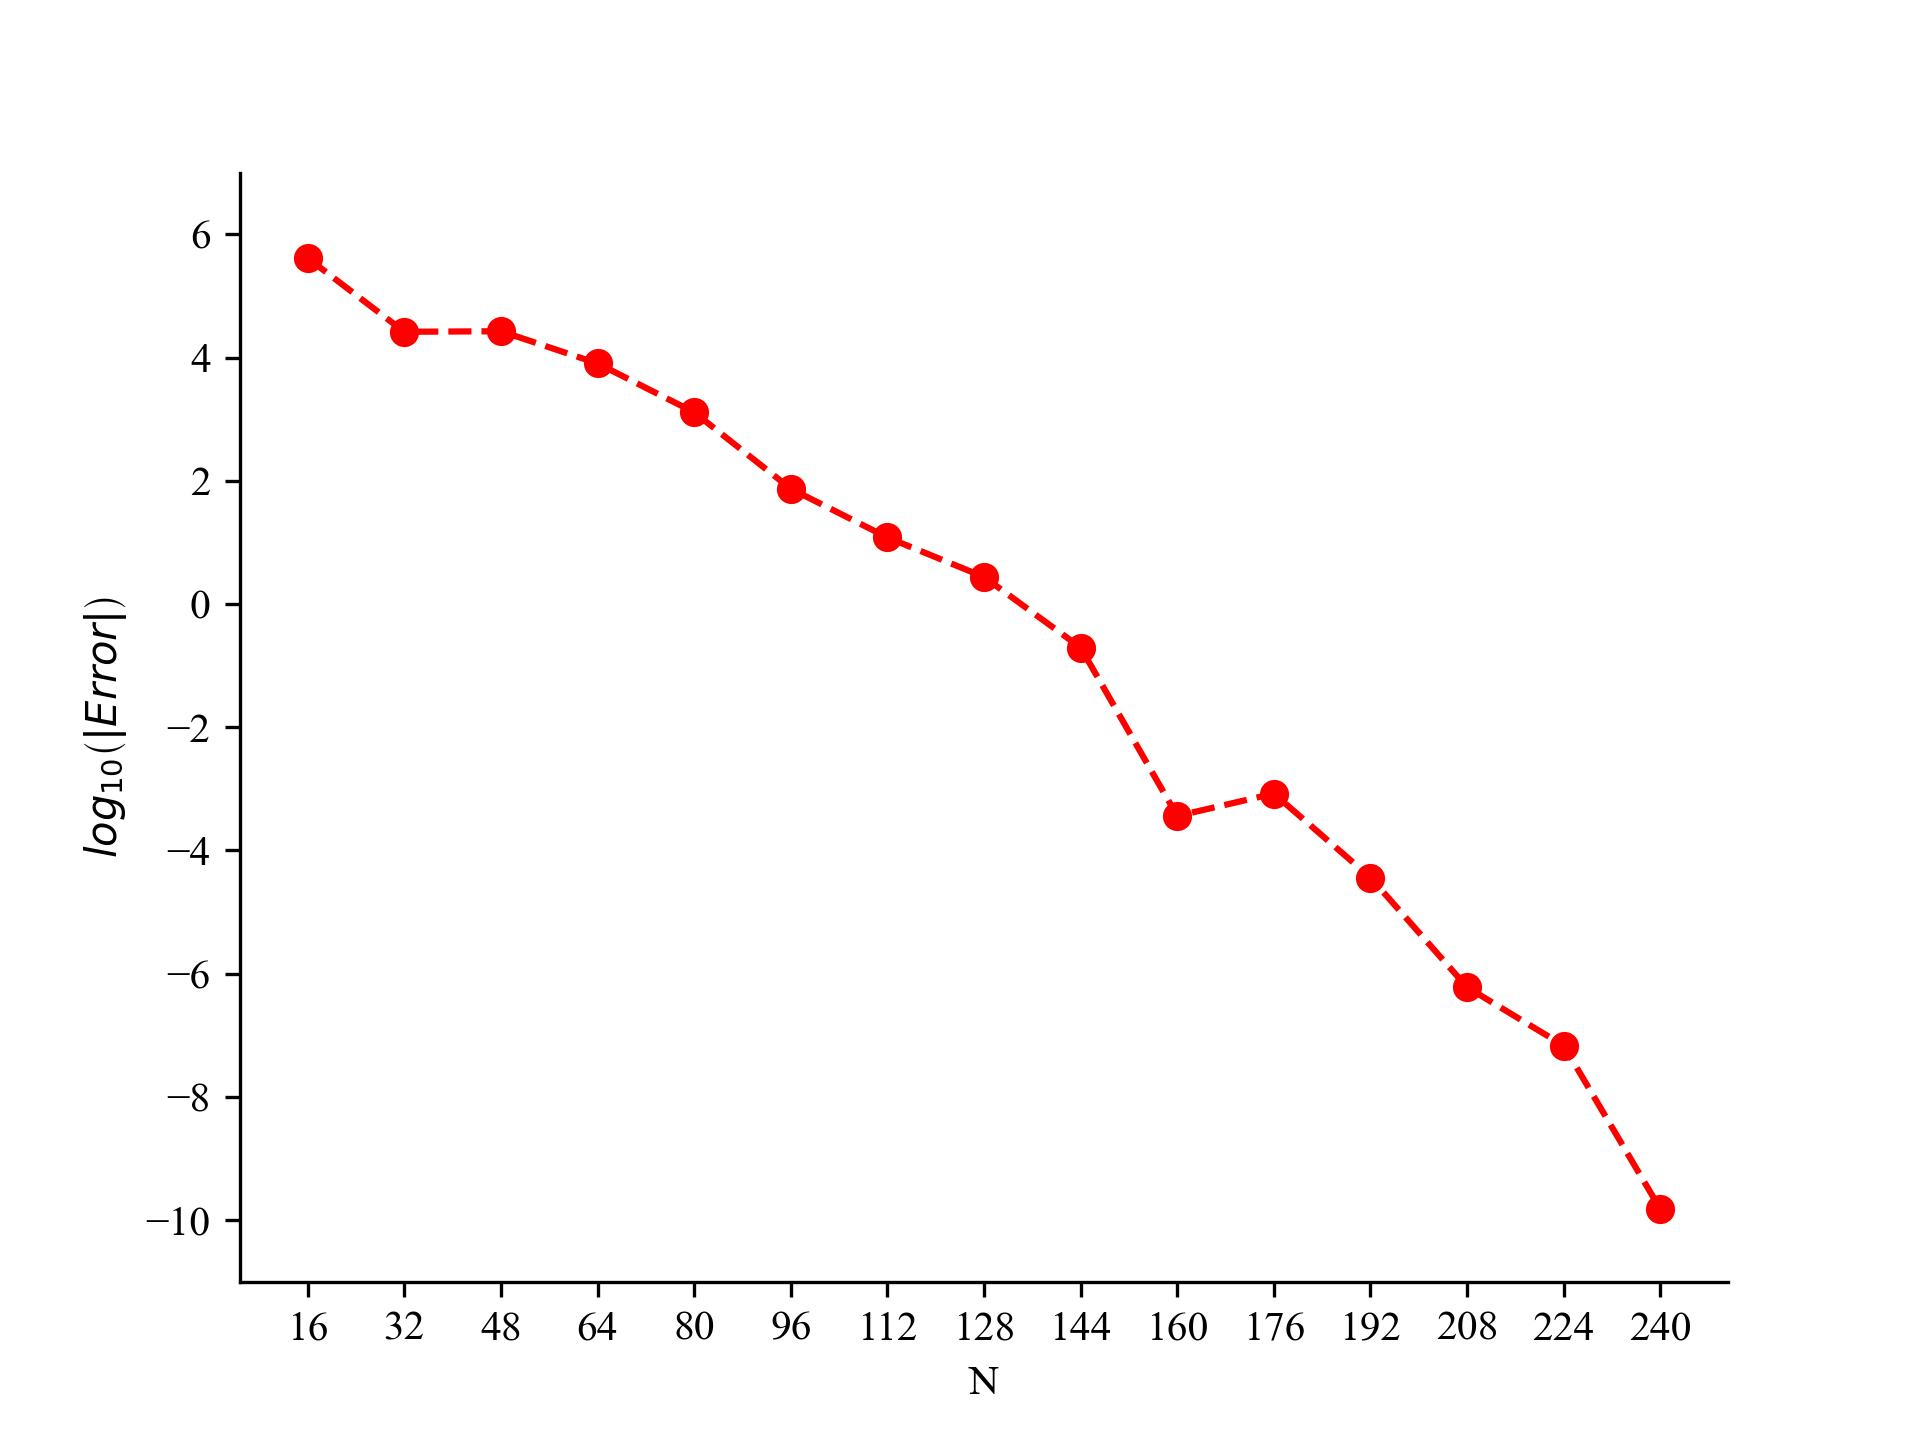
\includegraphics[width=0.8\linewidth]{error-plot-SVJ-call.jpg}
    \caption[\emph{SVJ-Call: The speed of error convergence.}]{\emph{SVJ-Call: The speed of error convergence.} \textbf{Note}: reference value $=10.5252142967$, criteria of negligible error from the product of payoff function and density is $10^{-15}$, $R^2=0.994$, and the regression line is $log_{10}\left(|Error|\right) = -2.395\times 10^{-5}N^2-0.0443N+5.1444$.}

    \label{fig:label}
\end{figure}



\subsection{Normal Inverse Gaussian Model}
\begin{figure}[H]
    \centering
    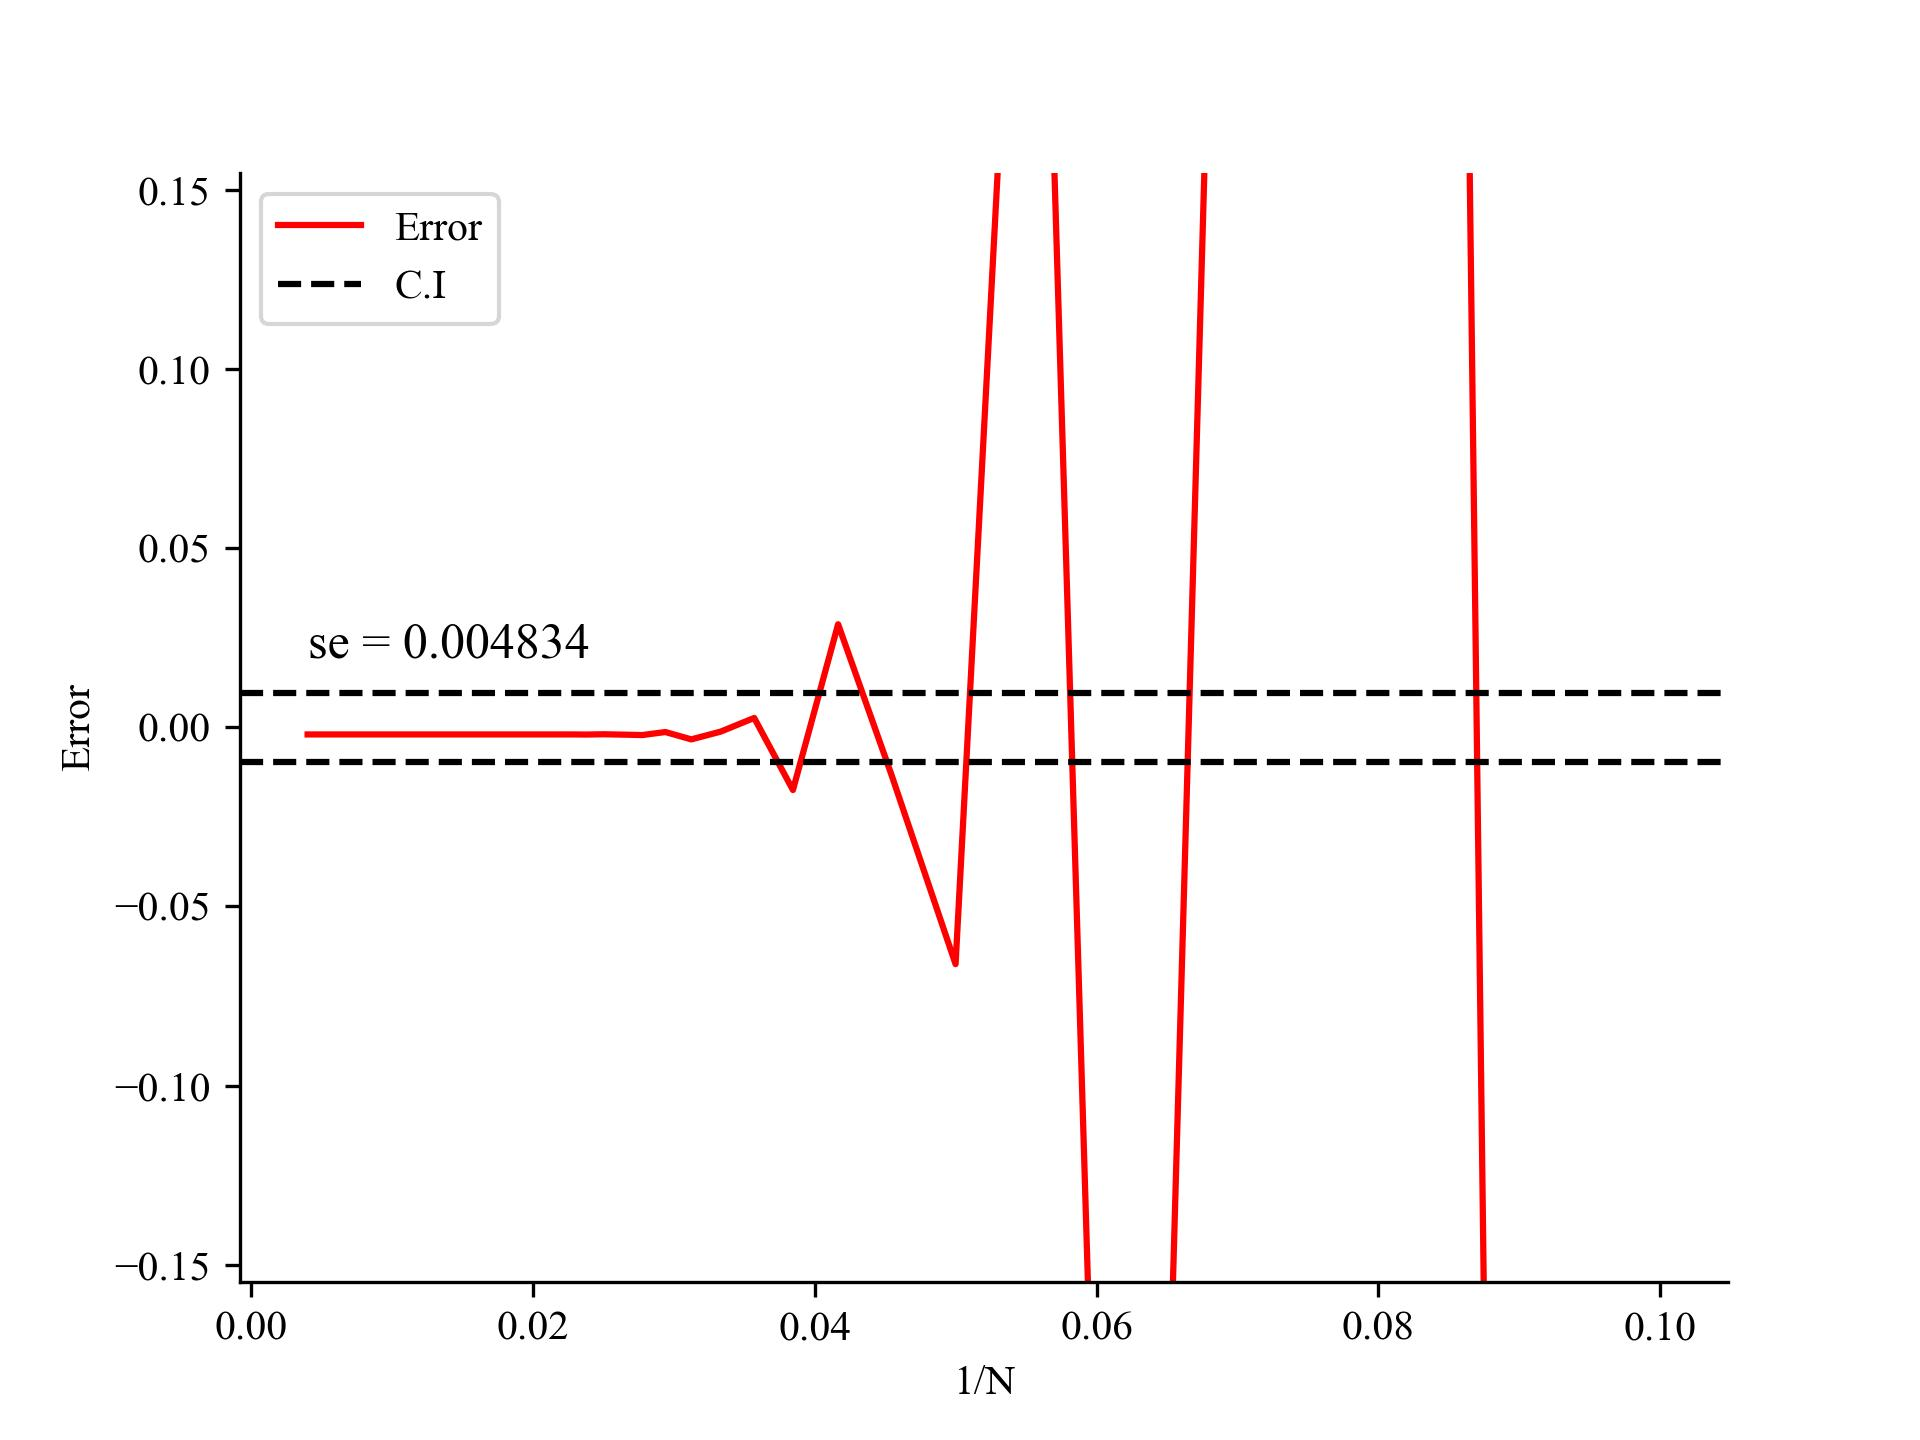
\includegraphics[width=0.8\linewidth]{value-plot-NIG-call.jpg}
     \caption[\emph{NIG-Call: Value accuracy comparing to the simulation with} $10^7$ \emph{paths.}]{\emph{NIG-Call: Value accuracy comparing to the simulation with} $10^7$ \emph{paths.} \textbf{Note}: mean value from simulation = 9.791681, criteria of negligible error from the product of payoff function and density is $10^{-6}$, and $N$ starts from $10$  with increment $=2$.}

    \label{fig:label}
\end{figure}
\begin{figure}[H]
    \centering
    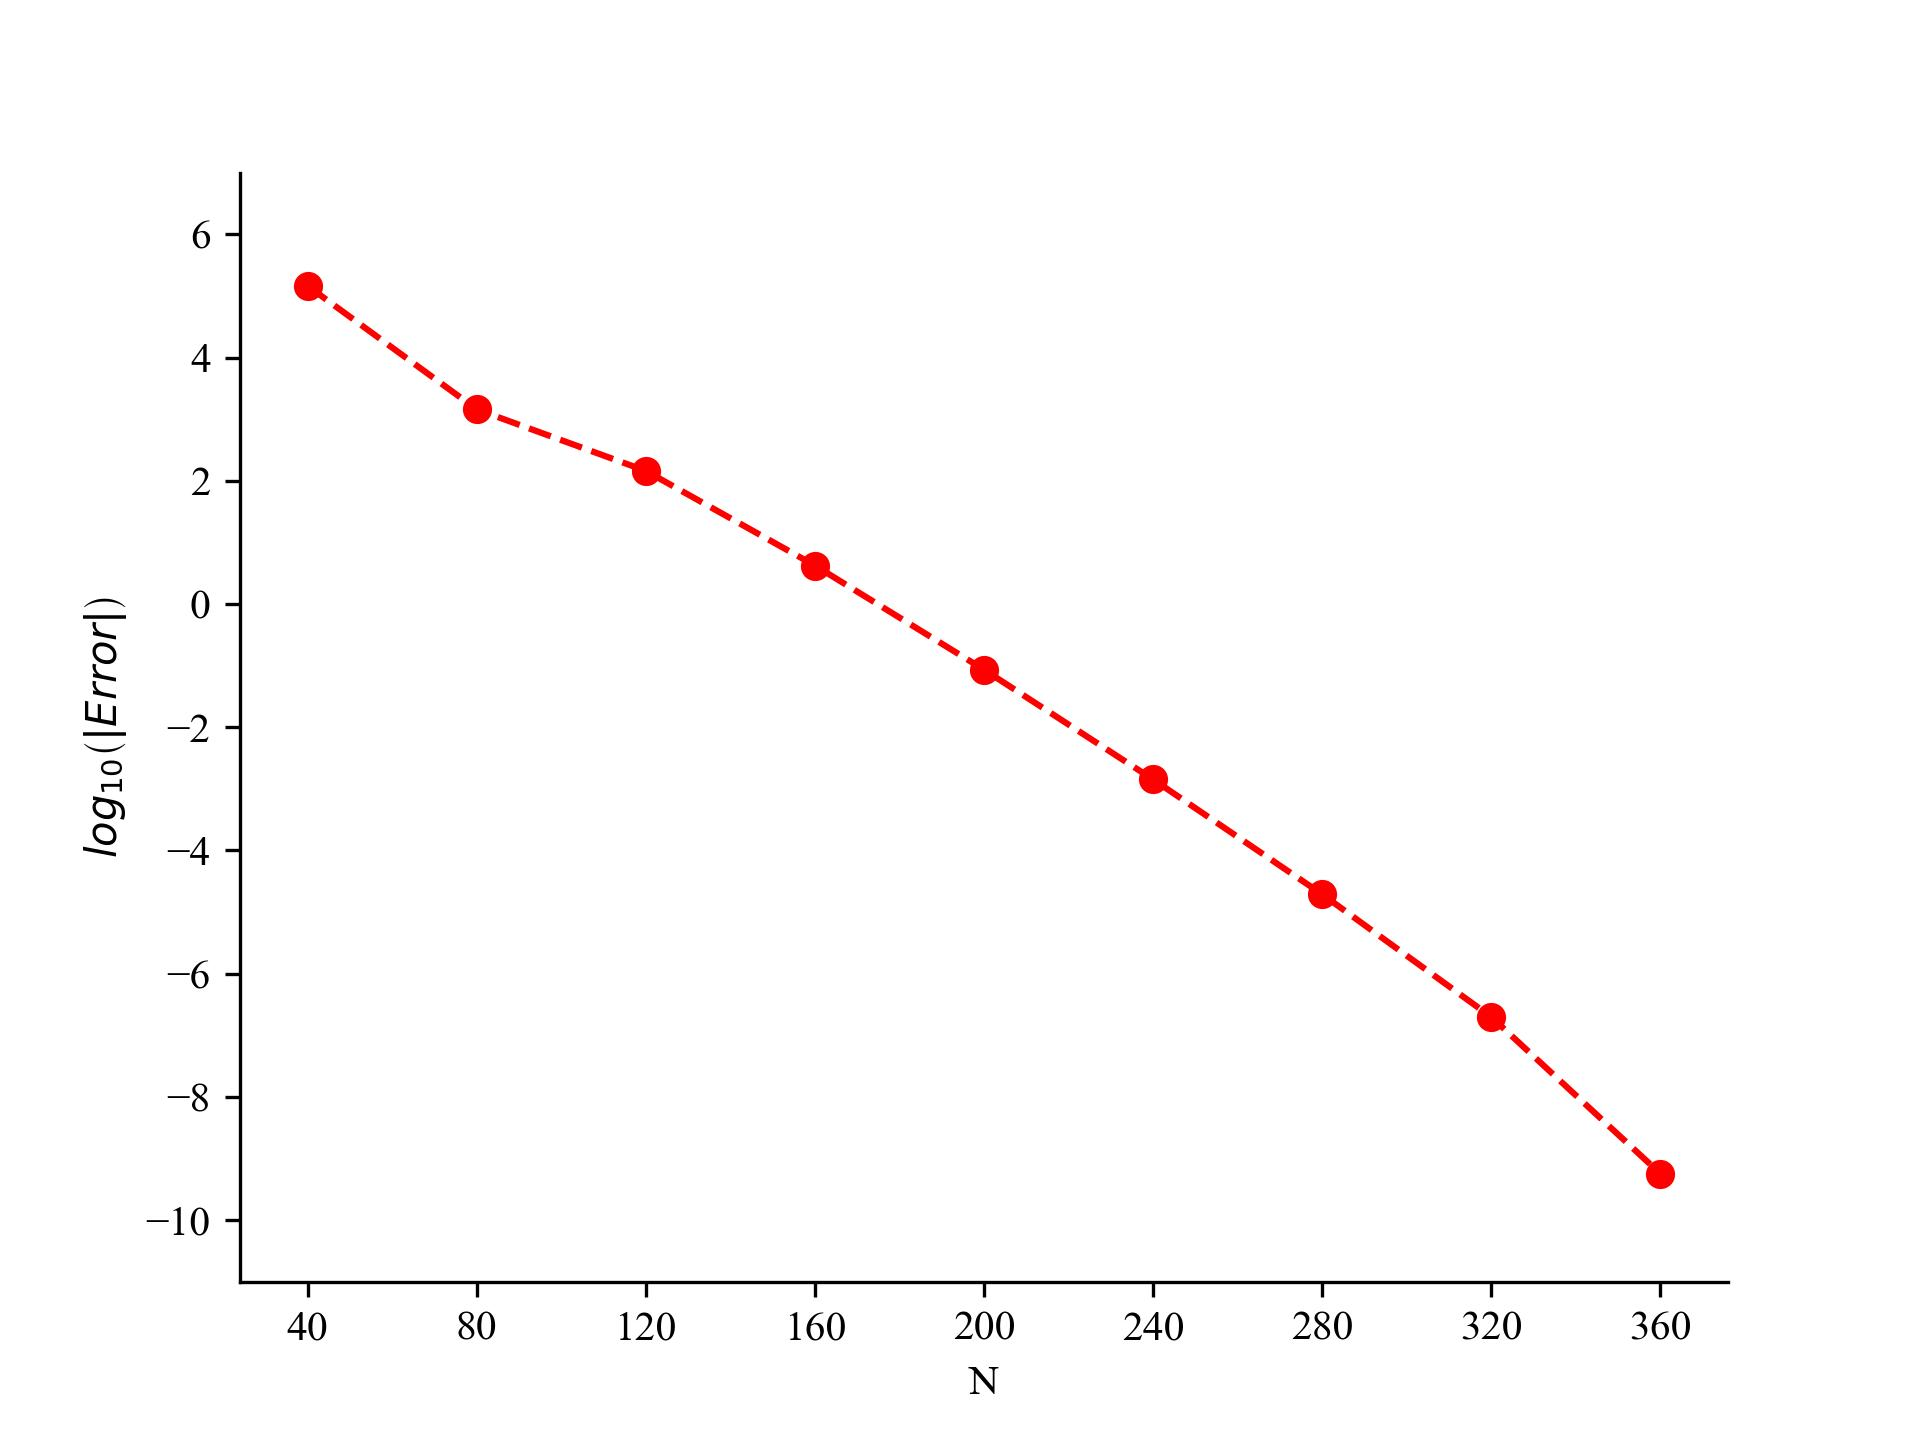
\includegraphics[width=0.8\linewidth]{error-plot-NIG-call.jpg}
    \caption[\emph{NIG-Call: The speed of error convergence.}]{\emph{NIG-Call: The speed of error convergence.} \textbf{Note}: reference value $=9.7896615158$, criteria of negligible error from the product of payoff function and density is $10^{-15}$, $R^2=0.991$, and the regression line is $log_{10}\left(|Error|\right) = 6.167\times 10^{-6}N^2-0.0562N+5.1576$.}
 
    \label{fig:label}
\end{figure}



\subsection{Variance Gamma Model}
\begin{figure}[H]
    \centering
    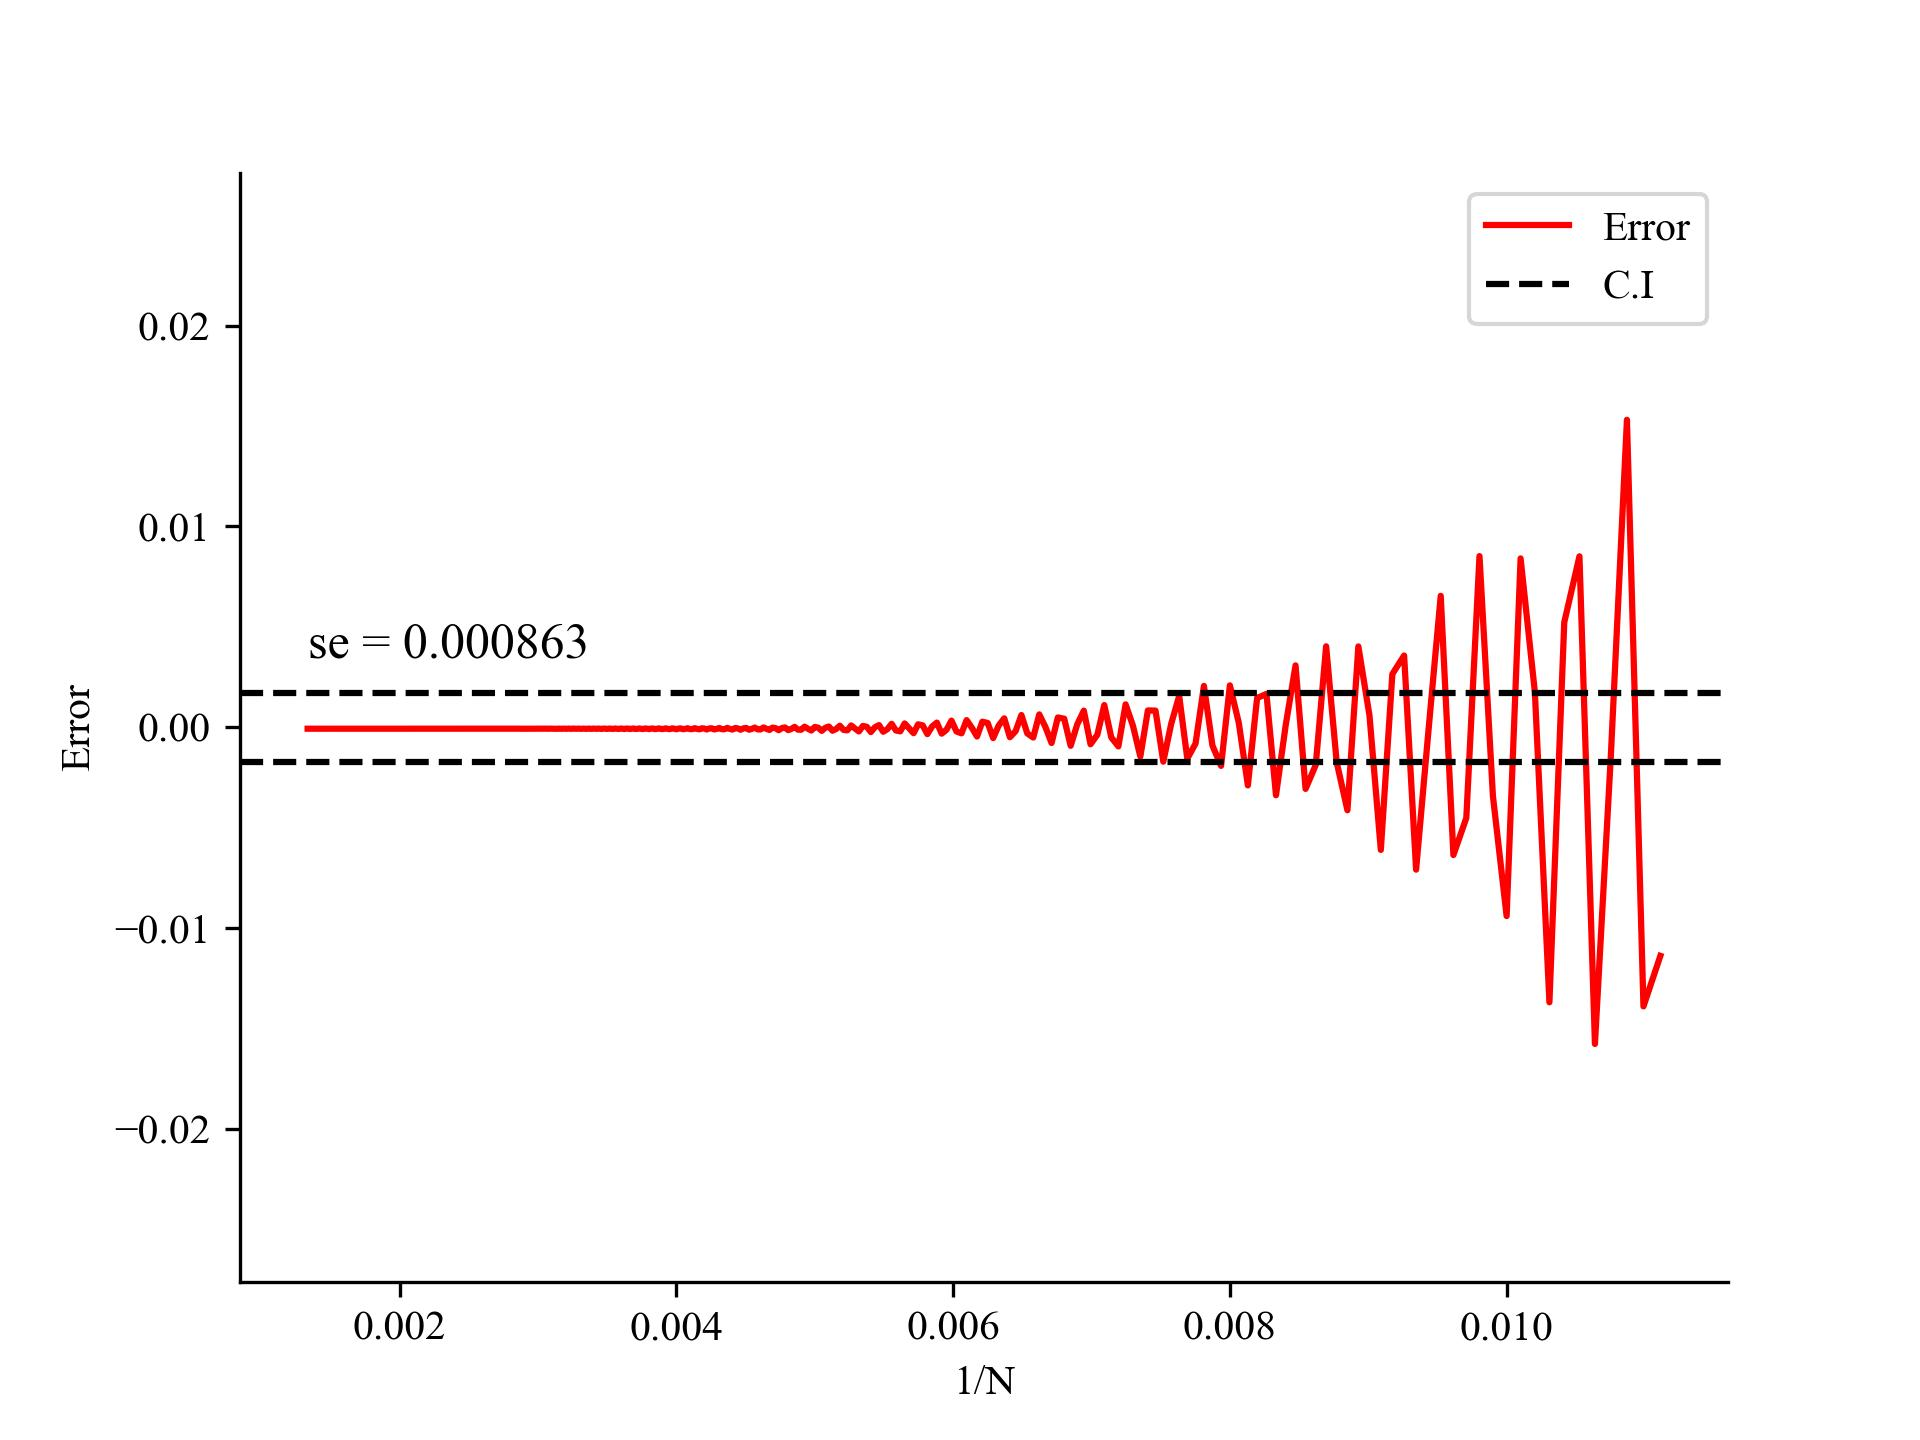
\includegraphics[width=0.8\linewidth]{value-plot-VG-call.jpg}
    \caption[\emph{VG-Call: Value accuracy comparing to the simulation with} $10^7$ \emph{paths.}]{\emph{VG-Call: Value accuracy comparing to the simulation with} $10^7$ \emph{paths.} \textbf{Note}: mean value from simulation = 6.885240, criteria of negligible error from the product of payoff function and density is $10^{-6}$, and $N$ starts from $10$  with increment $=2$.}
    
    \label{fig:label}
\end{figure}
\begin{figure}[H]
    \centering
    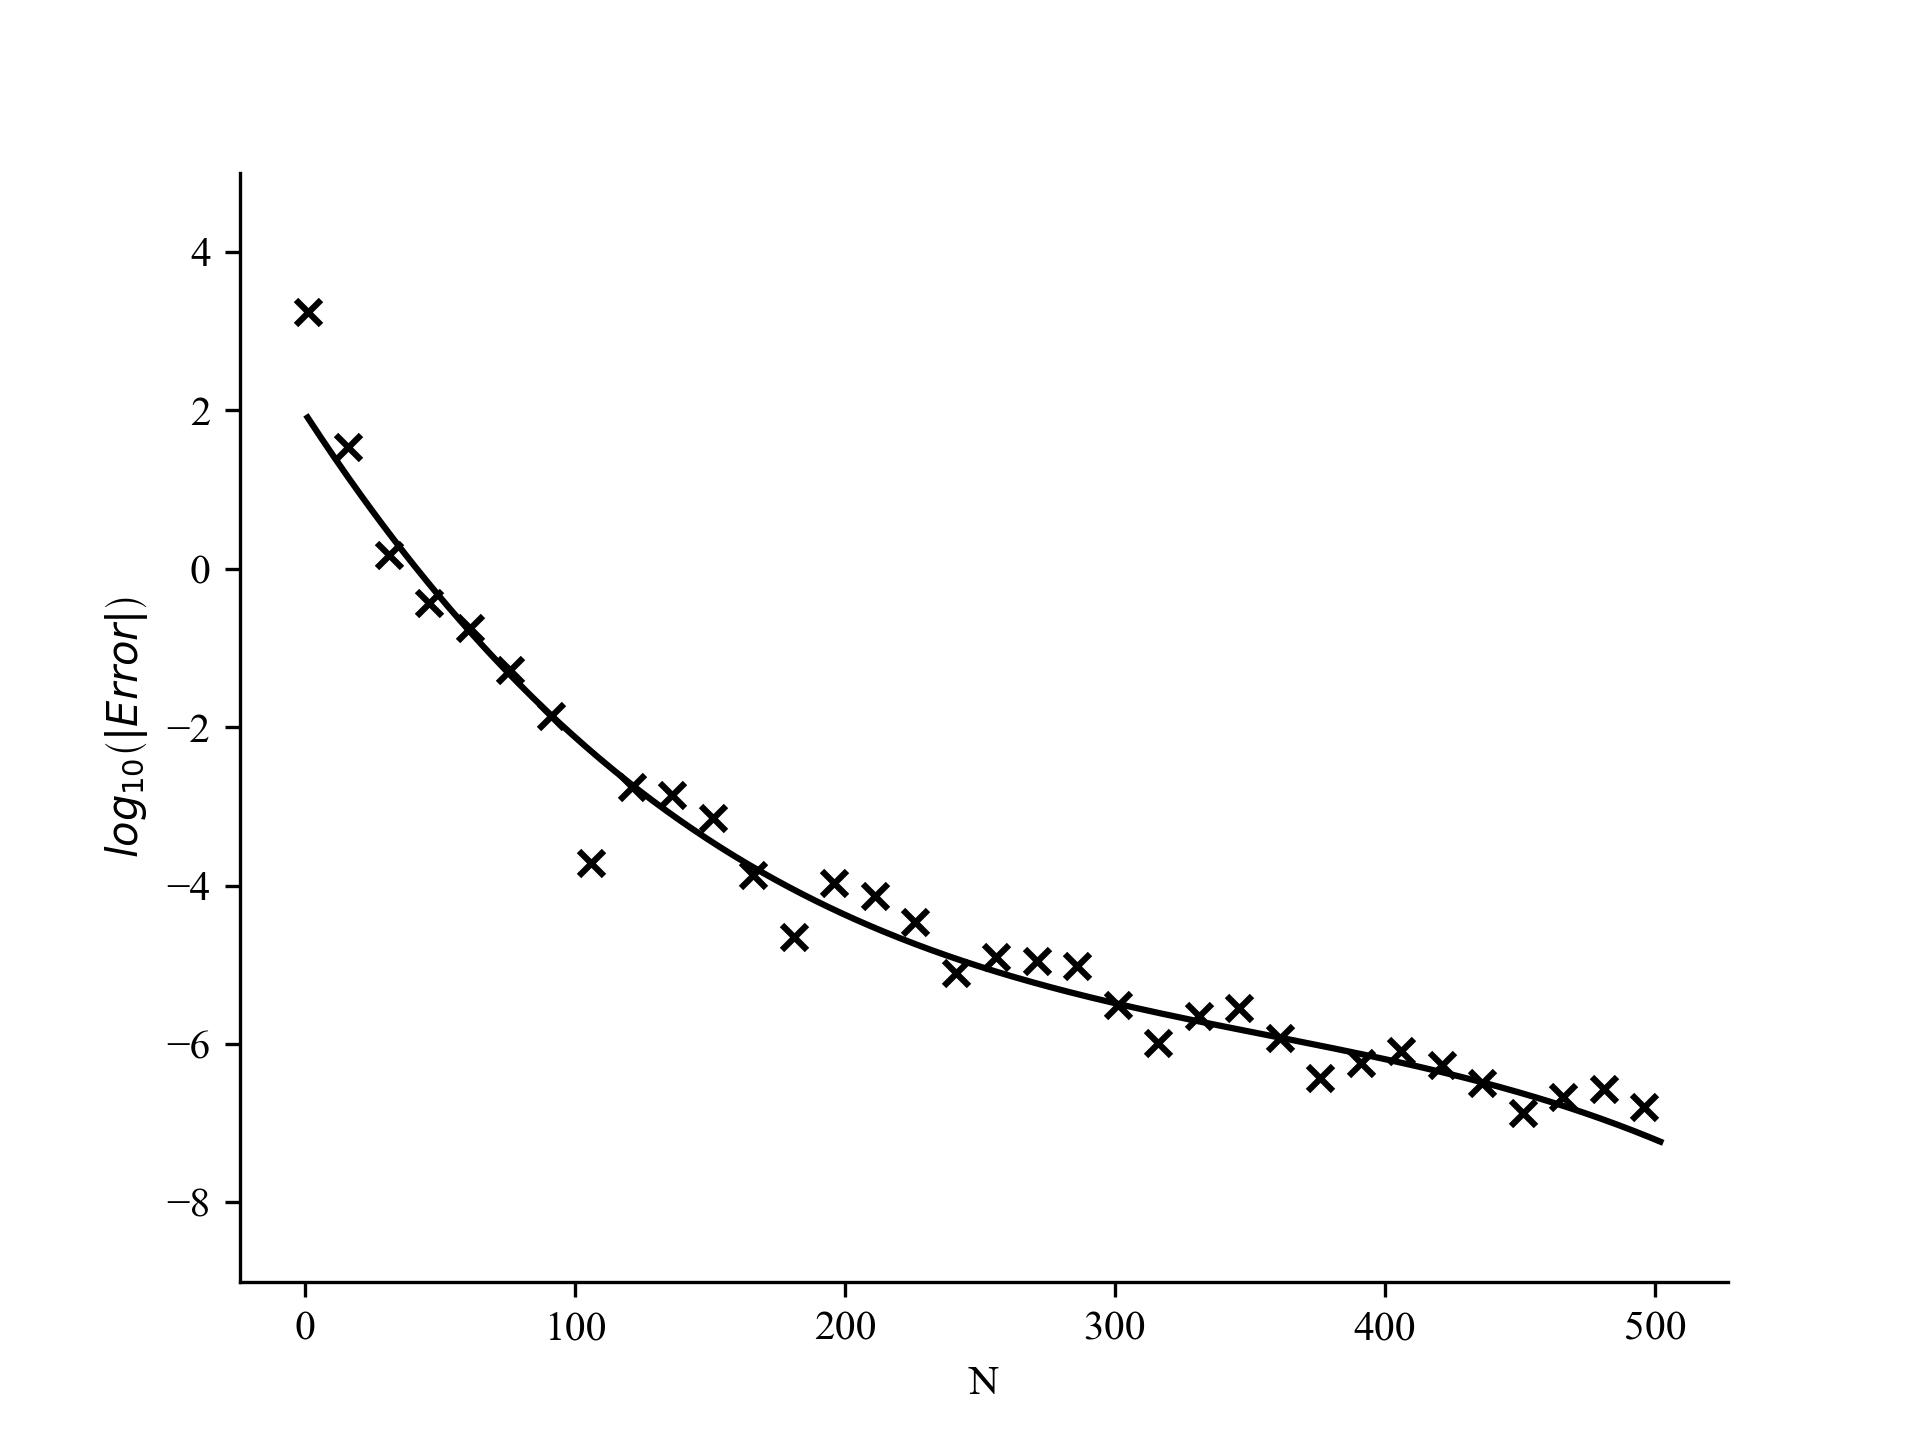
\includegraphics[width=0.8\linewidth]{error-plot-VG-call.jpg}
    \caption[\emph{VG-Call: The speed of error convergence.}]{\emph{VG-Call: The speed of error convergence.} \textbf{Note}: reference value $=6.8851648863$, criteria of negligible error from the product of payoff function and density is $10^{-15}$, $R^2=0.977$, and the regression line is $log_{10}\left(|Error|\right) = 0.0002N^2-0.07N+1.8948$.}

    \label{fig:label}
\end{figure}

\begin{figure}[ht]
    \begin{table}[H]
      \centering
      \caption[$log_{10}(|Error|)=AN^2+BN+C$]{Call - $log_{10}(|Error|)=AN^2+BN+C$}
    \end{table}
    
    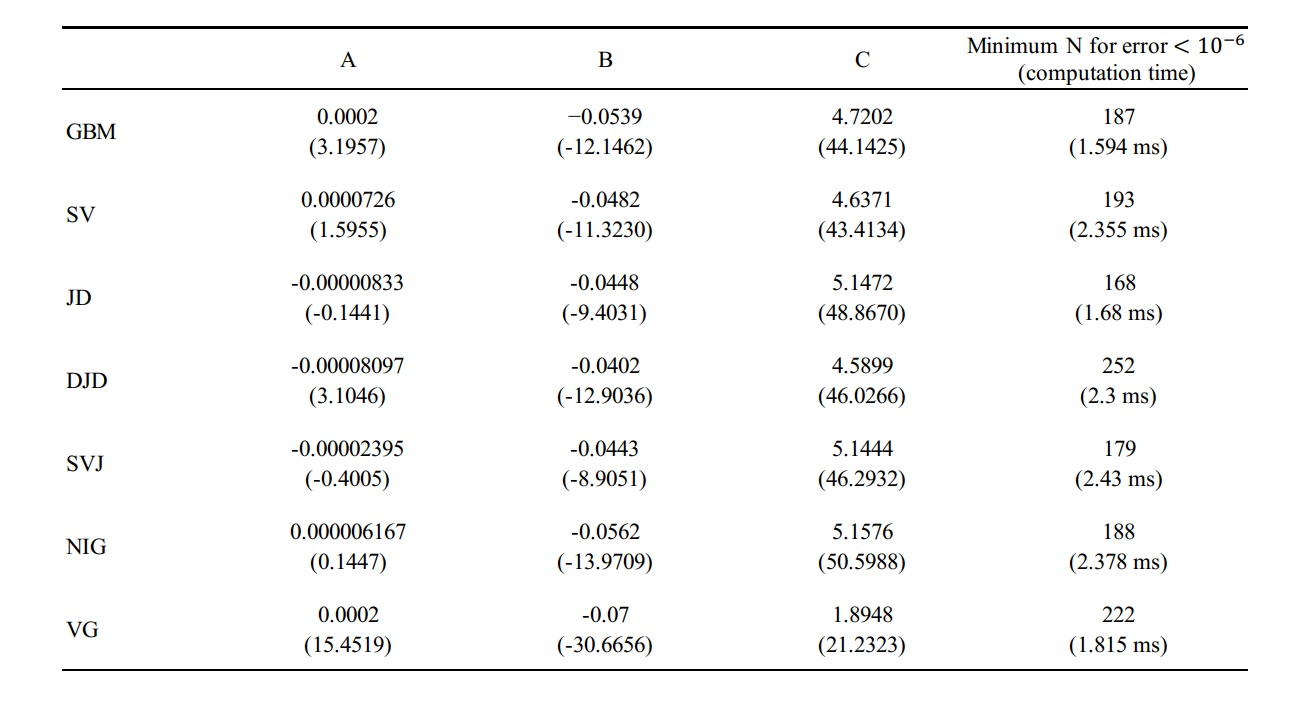
\includegraphics[width=1.1\textwidth,center]{call-table.jpg}
    \caption*{\small{This table reports the coefficients of the regression and t-statistics shown inside the parentheses in accordance with the coefficient. The time measurements in the final column are expressed in milliseconds and pertain to the MacBook Air equipped with the Apple M1 chip.}}
\end{figure}

% \begin{table}[ht]
% \caption[$log_{10}(|Error|)=AN^2+BN+C$]{Call - $log_{10}(|Error|)=AN^2+BN+C$}
% \centering
% \begin{tabular}{c c c }
%   \toprule
%   Coefficient 1 & Column 2 & Column 3 \\
%   \midrule
%   Value 1 & Value 2 & Value 3 \\
  
%   Value 4 & Value 5 & Value 6 \\
%   \bottomrule
% \end{tabular}
% \end{table}



I summarize the error convergence experimental results of the Call option in Table 3.1. The linear coefficients are all significantly negative, indicating that the model exhibits nearly exponential convergence. The quadratic coefficients, for the most part, are not significant, except for the geometric Brownian motion and the variance gamma model, but the coefficients are very small. Additionally, the computation time for all models is within 0.003 seconds, with an error on the order of $10^{-6}$. This demonstrates that the model is highly efficient for pricing call options.


\section{Convex Payoff for the Right End}
The one category of the payoff of the polynomial option is the convex payoff for the right end which has a payoff function where the leading coefficient is positive in $A \left(S_T\right)$. It means that the payoff function also tends to infinity as the stock price approaches infinity. As a polynomial option, the curve on the far right of the payoff function must be convex, meaning that the function has an infinite value on the right side. I call this category "Right Up".

To examine this polynomial option, the setting is $A(S_T)=0.05S_T^2-5S_T-20$. Then, the roots of $A(S_T)$ is $10\left( 5 - \sqrt{29} \right)$ and $10\left( 5 + \sqrt{29} \right)$. As a result, the positive interval that can be obtained $\left[0, \, 10\left( 5 - \sqrt{29} \right)\right]$, and $\left[ \, 10\left( 5 + \sqrt{29} \right),  \,\infty \right]$. All the following experiments are under $S_0=90$.

Note that the reference values for analyzing error convergence are calculated using binomial tree only for geometric Brownian motion. For other stochastic processes, these values are calculated under my model with $N=10^5$, because there are no analytical solution or tree-based methods for pricing polynomial options aside from geometric Brownian motion. These values fall within the confidence interval constructed by simulating $10^7$ paths within two standard errors. 

\newpage

\subsection{Geometric Brownian Motion}
\begin{figure}[H]
    \centering
    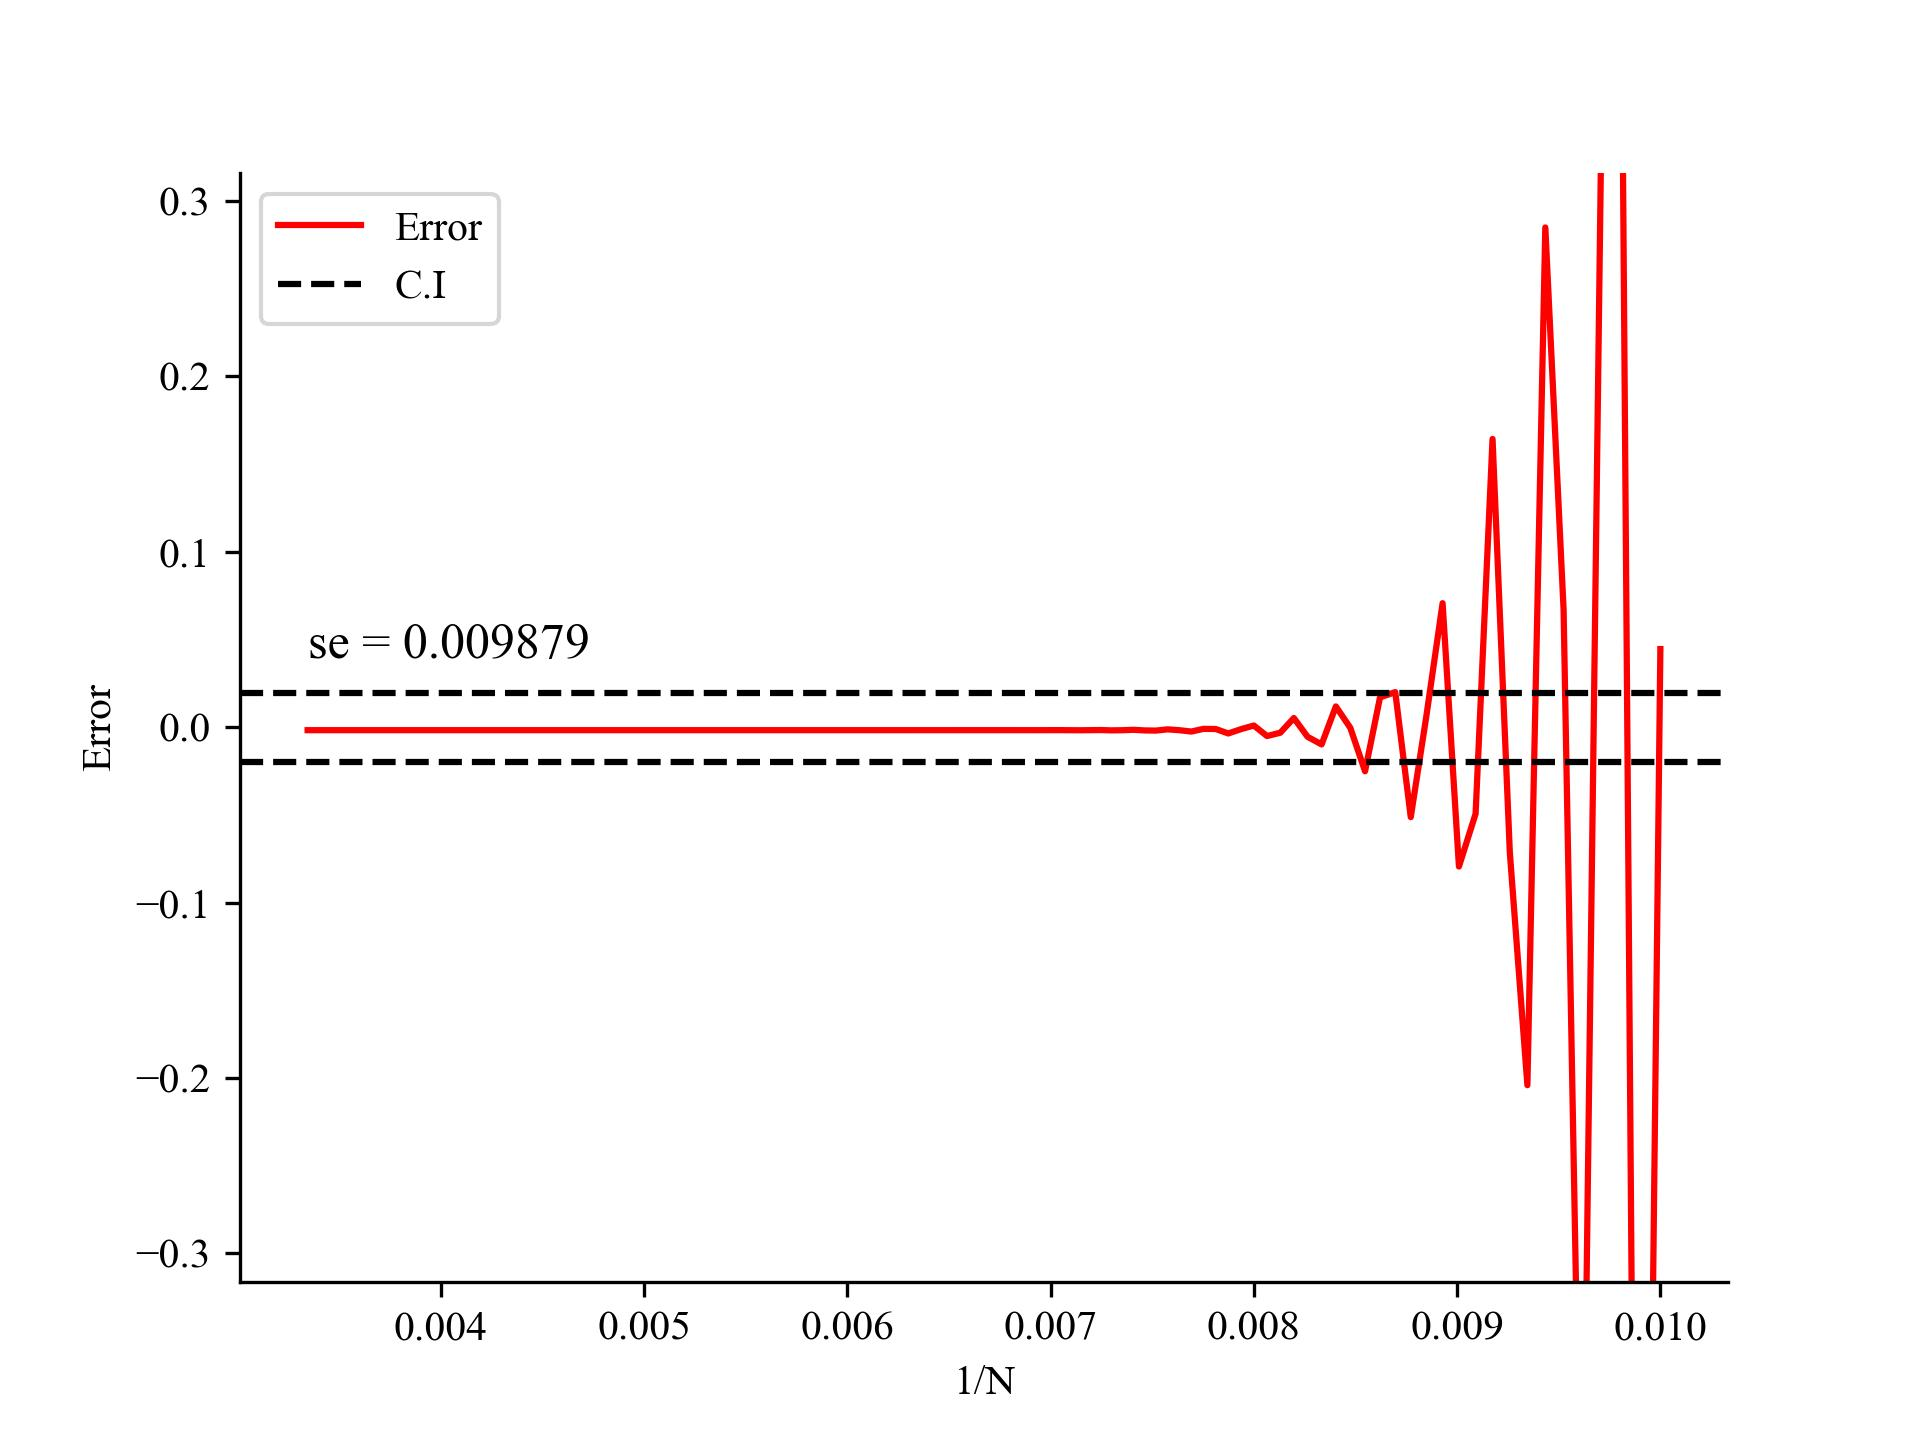
\includegraphics[width=0.8\linewidth]{value-plot-GBM-rightup.jpg}
    \caption[\emph{GBM-Up: Value accuracy comparing to the simulation with} $10^7$ \emph{paths.}]{\emph{GBM-Up: Value accuracy comparing to the simulation with} $10^7$ \emph{paths.} \textbf{Note}: mean value from simulation = 9.363655, criteria of negligible error from the product of payoff function and density is $10^{-6}$, and $N$ starts from $10$  with increment $=2$.}

    \label{fig:label}
\end{figure}

\begin{figure}[H]
    \centering
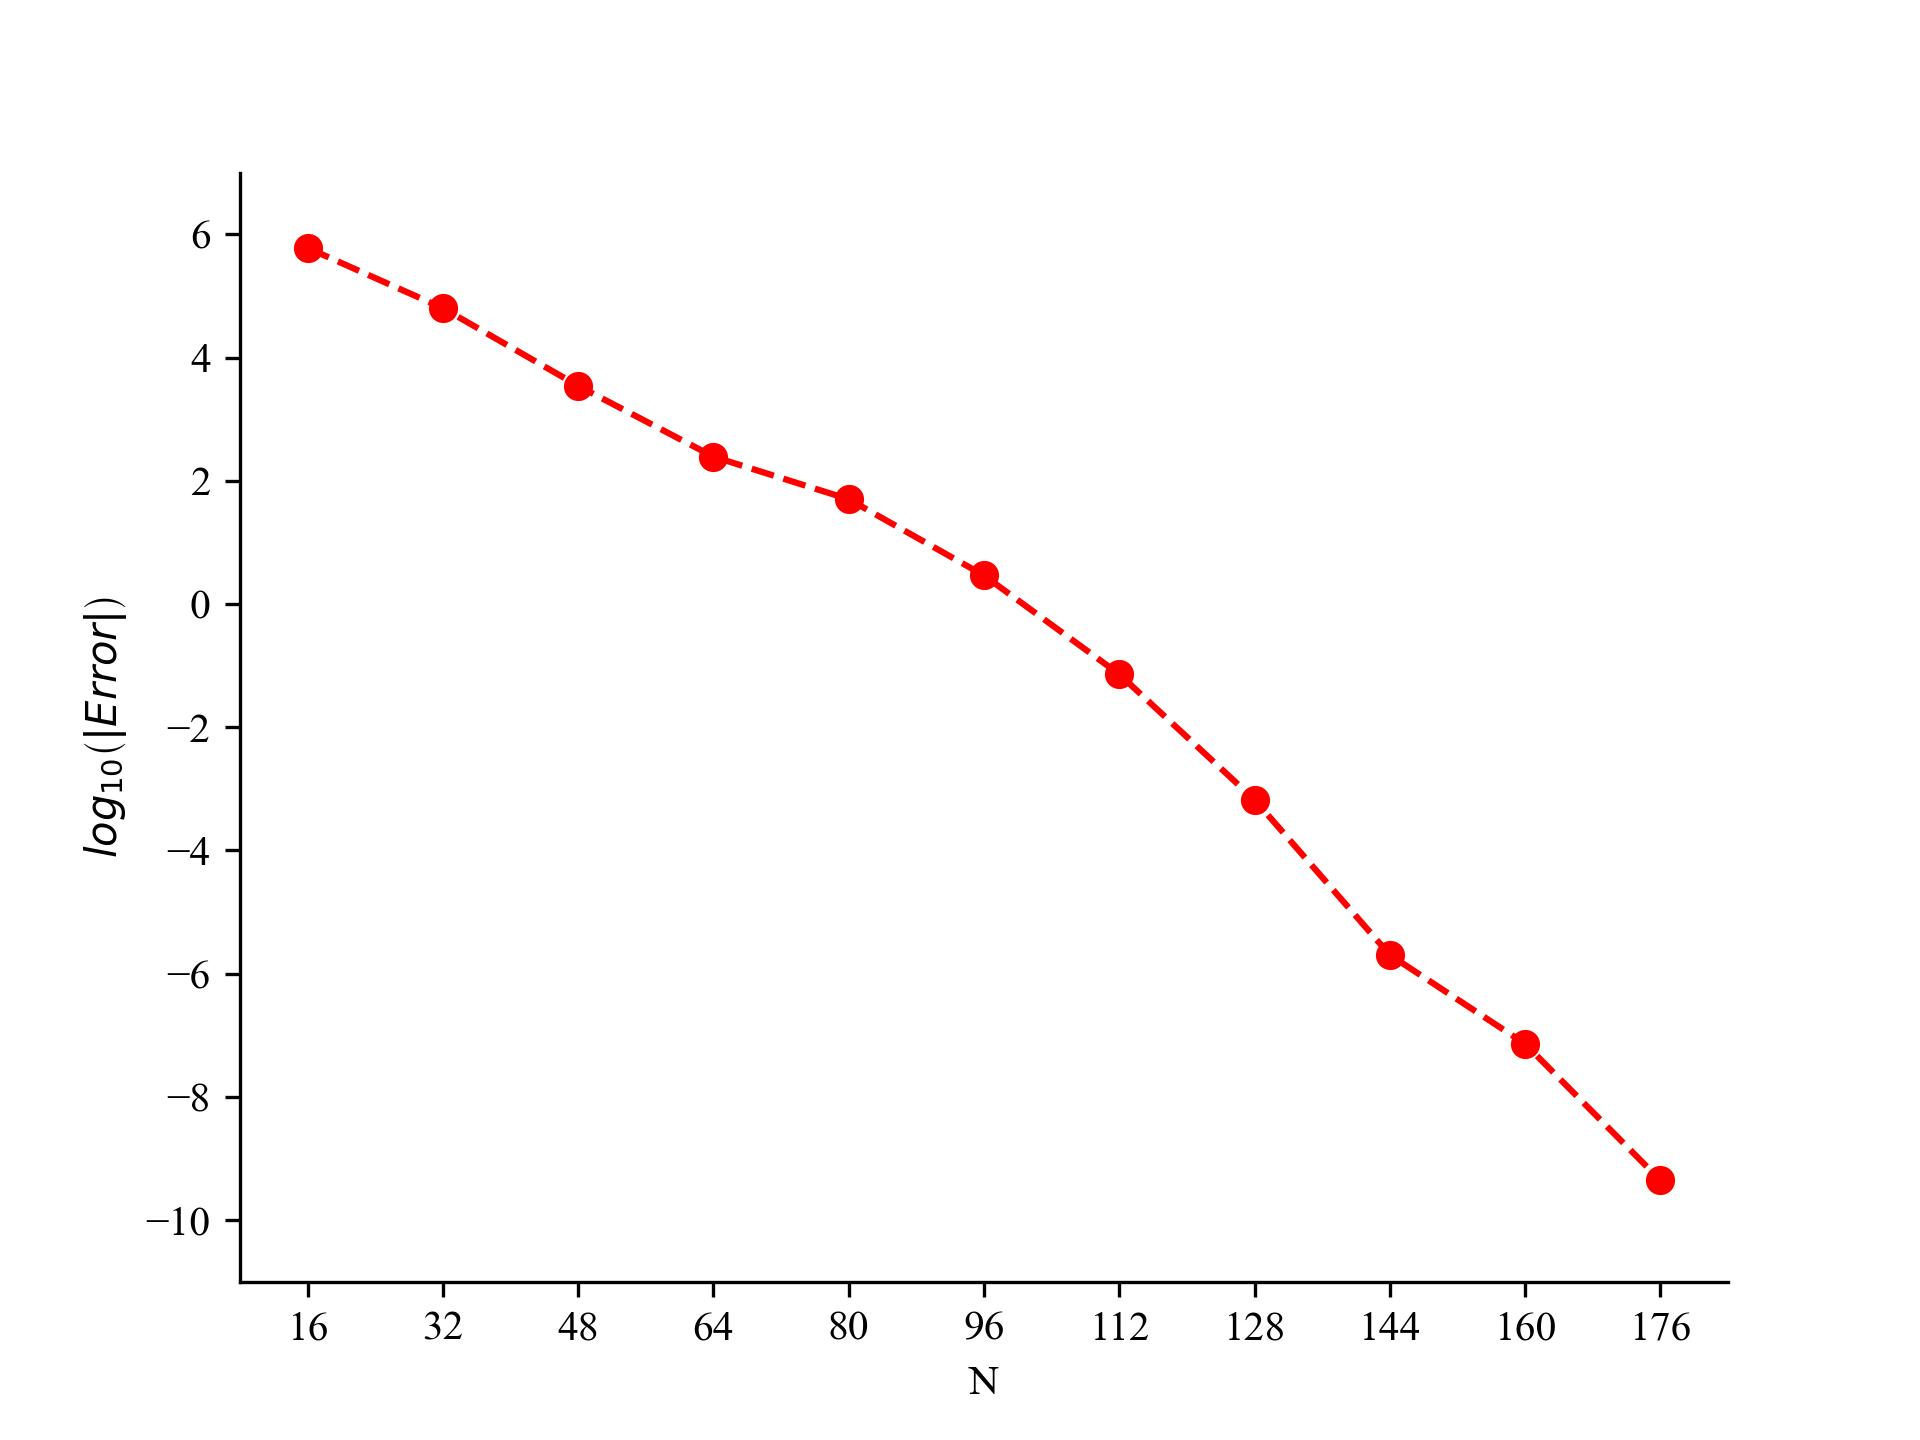
\includegraphics[width=0.8\linewidth]{error-plot-GBM-rightup.jpg}
    \caption[\emph{GBM-Up: The speed of error convergence.}]{\emph{GBM-Up: The speed of error convergence.} \textbf{Note}: reference value $=9.3619657891$, criteria of negligible error from the product of payoff function and density is $10^{-15}$, $R^2=0.995$, and the regression line is $log_{10}\left(|Error|\right) = -1.837\times 10^{-5}N^2-0.0295N+7.9392$.}

    \label{fig:label}
\end{figure}


\subsection{Stochastic Volatility Model}
\begin{figure}[H]
    \centering
    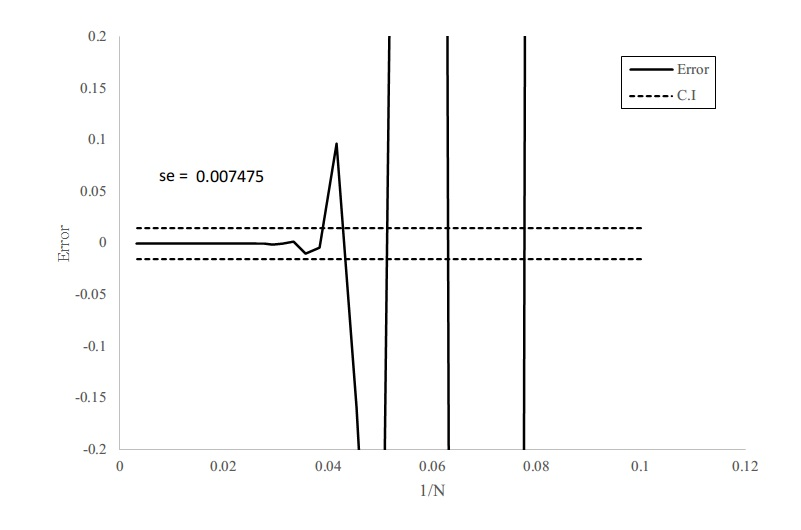
\includegraphics[width=0.8\linewidth]{value-plot-Heston-rightup.jpg}
    \caption[\emph{SV-Up: Value accuracy comparing to the simulation with} $10^7$ \emph{paths.}]{\emph{SV-Up: Value accuracy comparing to the simulation with} $10^7$ \emph{paths.} \textbf{Note}: mean value from simulation = 9.218680, criteria of negligible error from the product of payoff function and density is $10^{-6}$, and $N$ starts from $10$  with increment $=2$.}

    \label{fig:label}
\end{figure}
\begin{figure}[H]
    \centering
    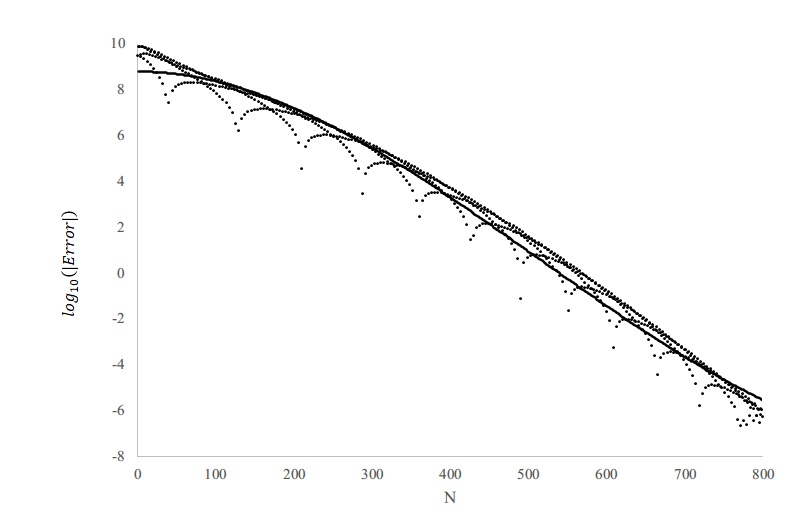
\includegraphics[width=0.8\linewidth]{error-plot-Heston-rightup.jpg}
    \caption[\emph{SV-Up: The speed of error convergence.}]{\emph{SV-Up: The speed of error convergence.} \textbf{Note}: reference value $=9.2180914622$, criteria of negligible error from the product of payoff function and density is $10^{-15}$, $R^2=0.994$, and the regression line is $log_{10}\left(|Error|\right) = -1.102\times 10^{-5}N^2-0.0107N+9.4685$.}
    
    \label{fig:label}
\end{figure}




\subsection{Log-normal Jump Diffusion Model}
\begin{figure}[H]
    \centering
    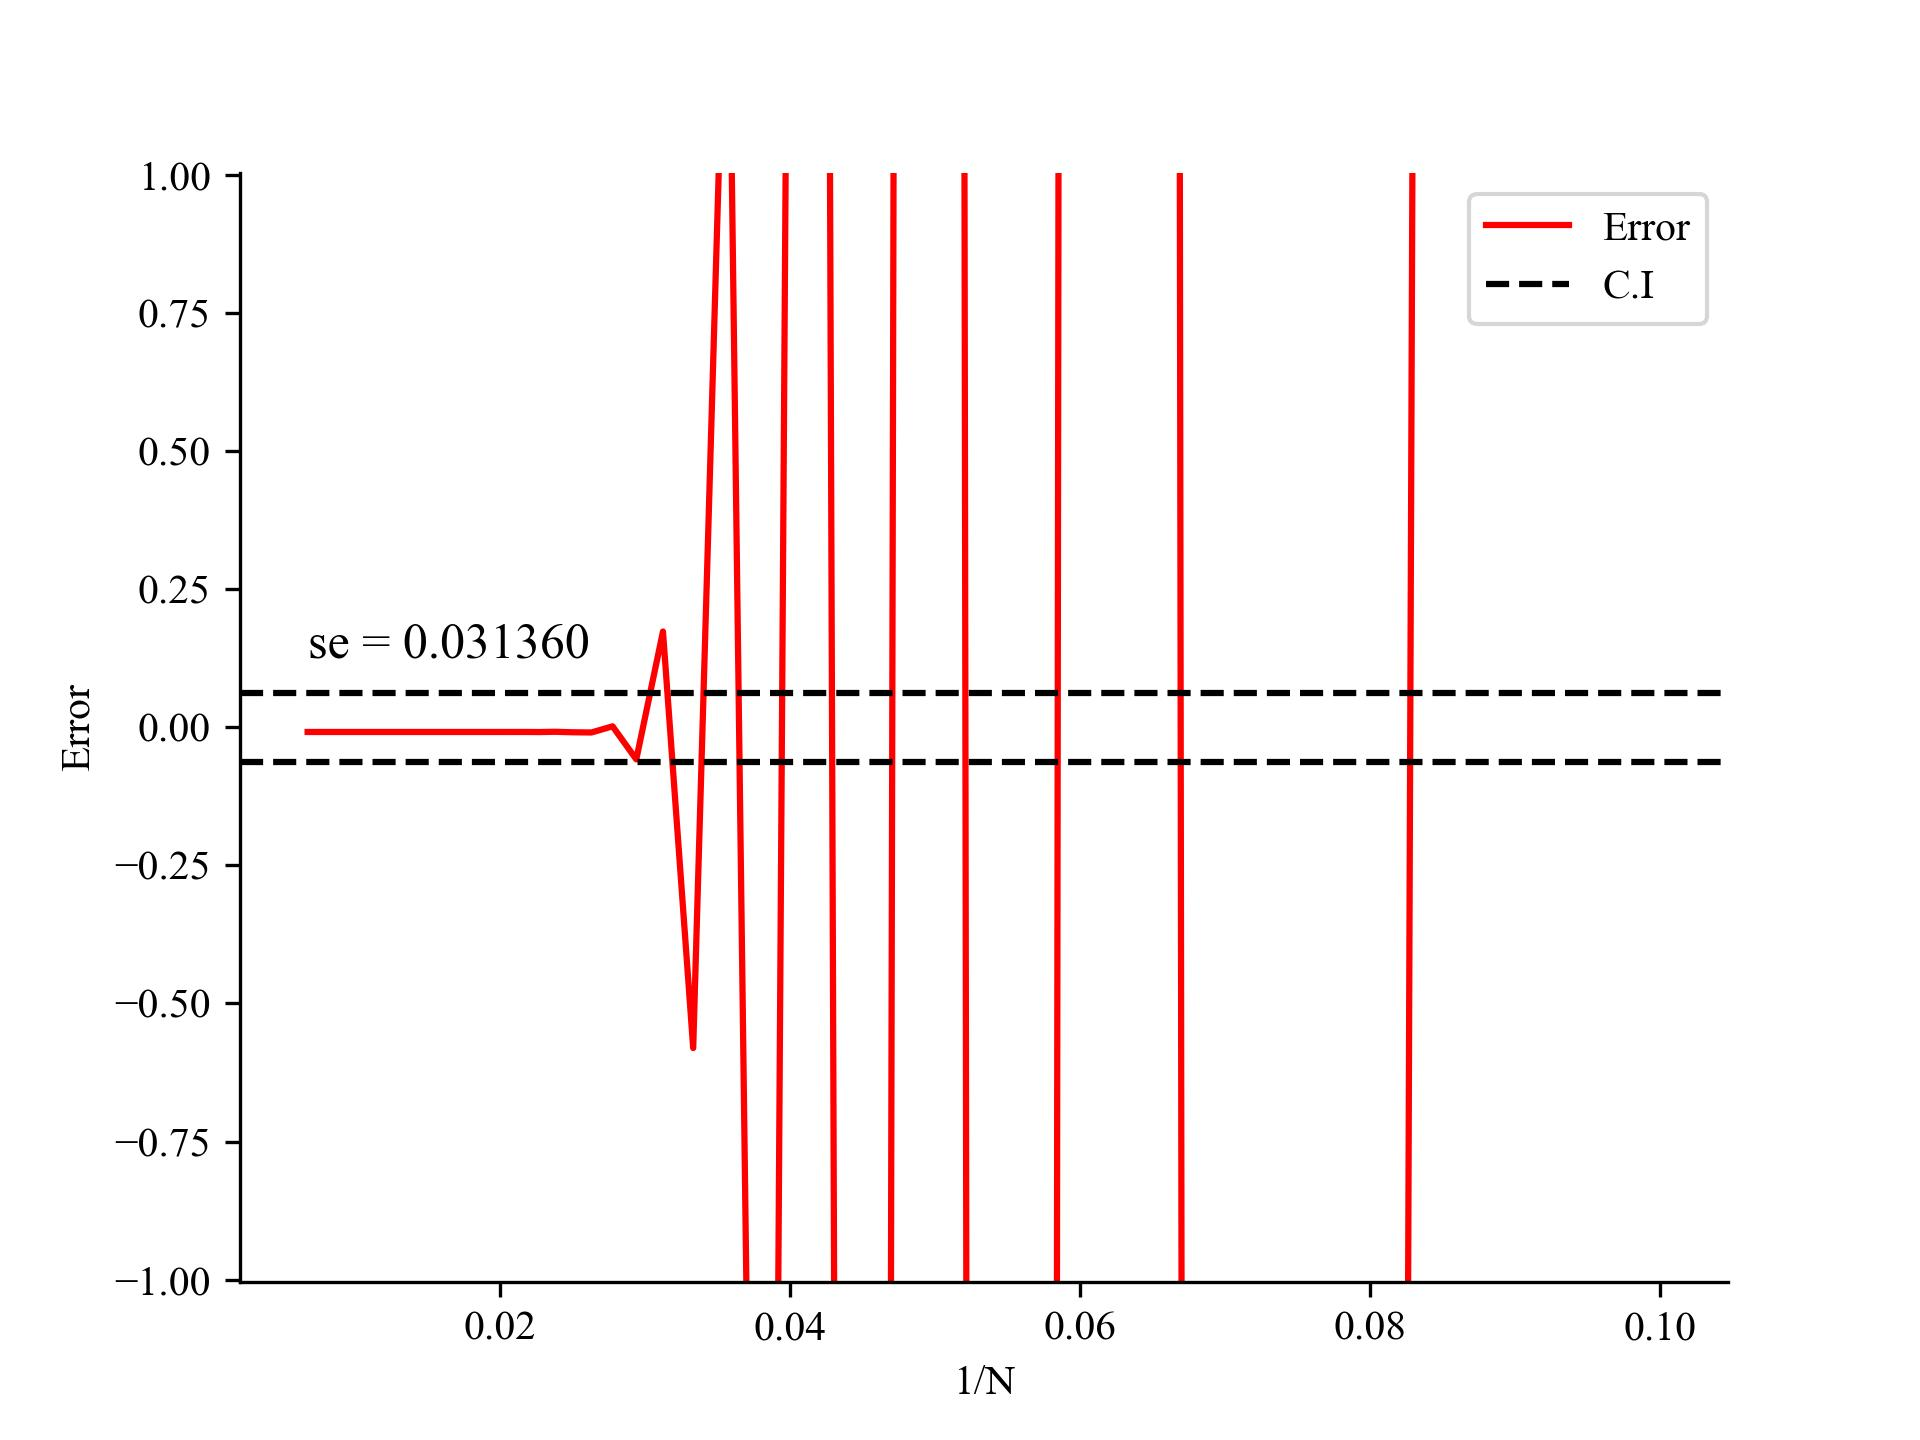
\includegraphics[width=0.8\linewidth]{value-plot-MJD-rightup.jpg}
    \caption[\emph{JD-Up: Value accuracy comparing to the simulation with} $10^7$ \emph{paths.}]{\emph{JD-Up: Value accuracy comparing to the simulation with} $10^7$ \emph{paths.} \textbf{Note}: mean value from simulation = 31.191878, criteria of negligible error from the product of payoff function and density is $10^{-6}$, and $N$ starts from $10$  with increment $=2$.}
    
    \label{fig:label}
\end{figure}

\begin{figure}[H]
    \centering
    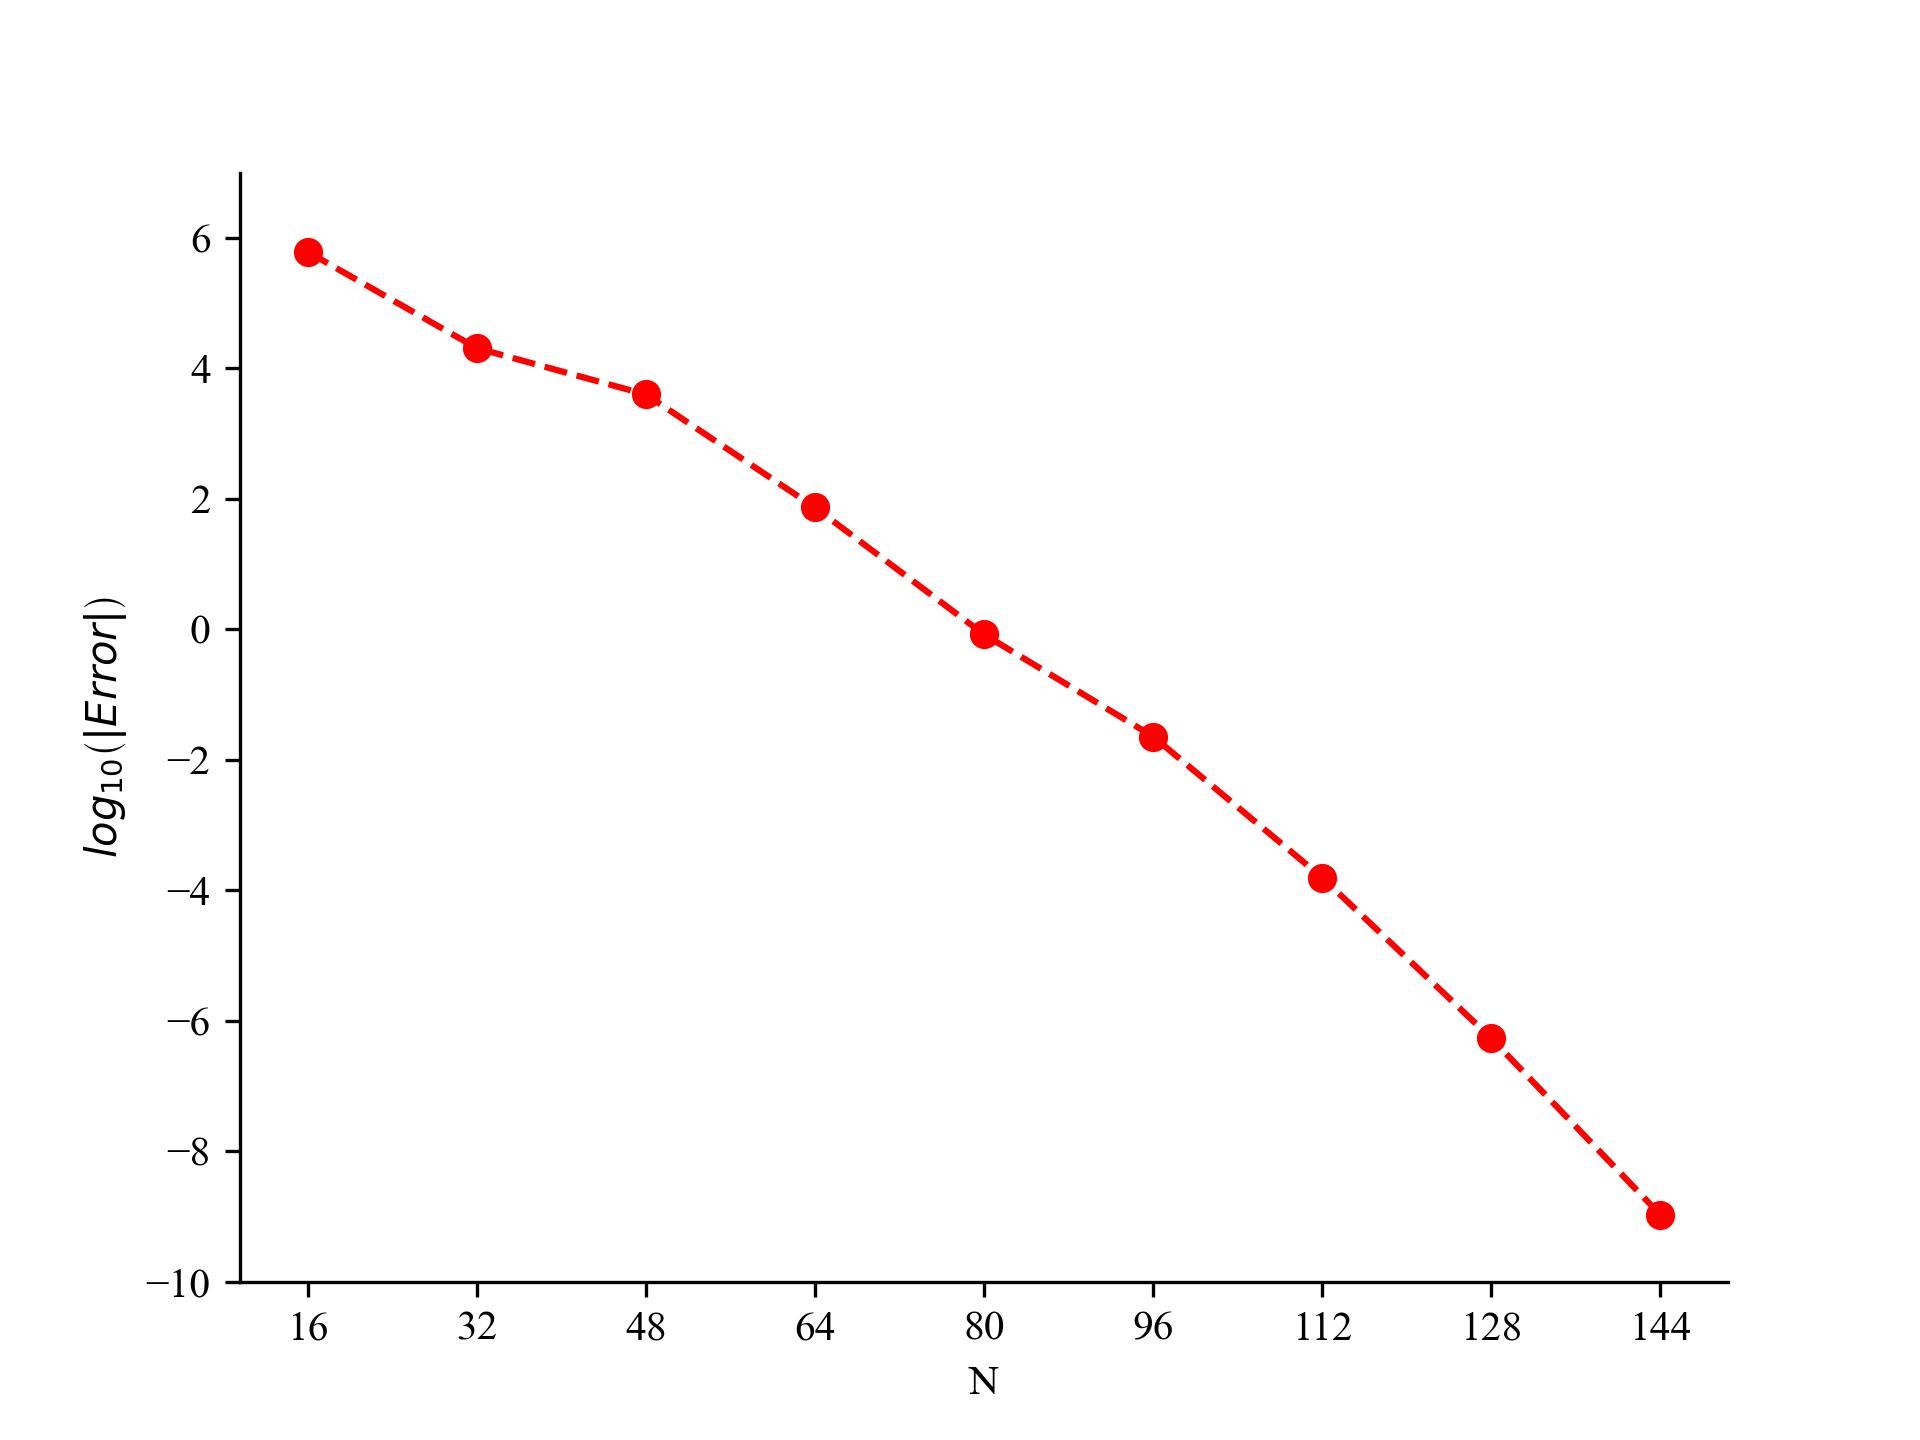
\includegraphics[width=0.8\linewidth]{error-plot-MJD-rightup.jpg}
    \caption[\emph{JD-Up: The speed of error convergence.}]{\emph{JD-Up: The speed of error convergence.} \textbf{Note}: reference value $=31.1831933197$, criteria of negligible error from the product of payoff function and density is $10^{-15}$, $R^2=0.996$, and the regression line is $log_{10}\left(|Error|\right) = -0.0003N^2-0.0367N+9.6889$.}

    \label{fig:label}
\end{figure}


\subsection{Double Exponential Jump Diffusion Model}
\begin{figure}[H]
    \centering
    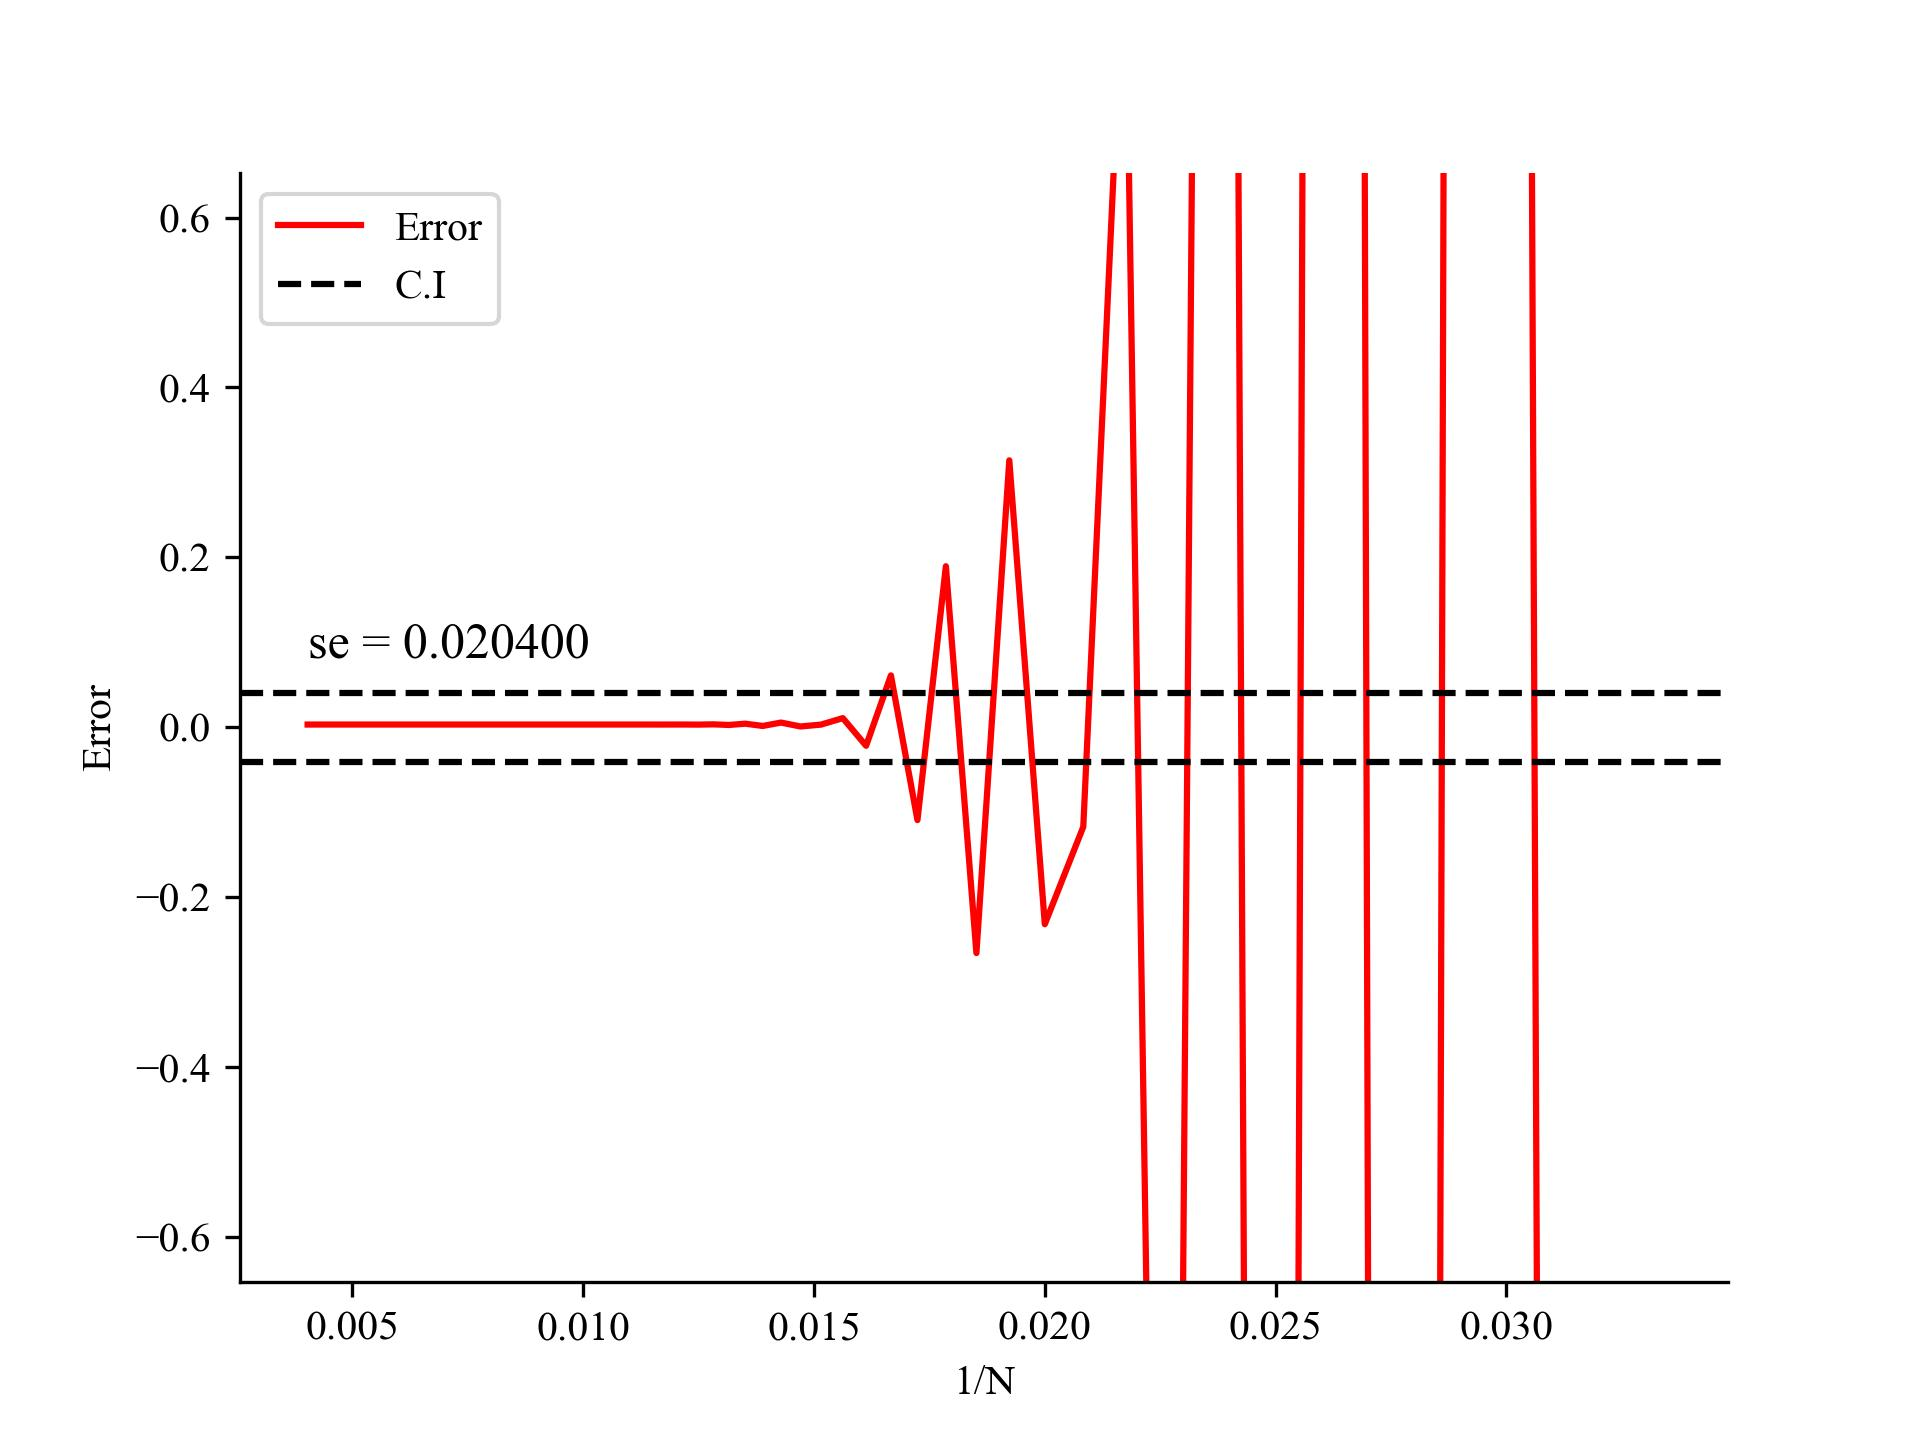
\includegraphics[width=0.8\linewidth]{value-plot-KJD-rightup.jpg}
     \caption[\emph{DJD-Up: Value accuracy comparing to the simulation with} $10^7$ \emph{paths.}]{\emph{DJD-Up: Value accuracy comparing to the simulation with} $10^7$ \emph{paths.} \textbf{Note}: mean value from simulation = 18.122275, criteria of negligible error from the product of payoff function and density is $10^{-6}$, and $N$ starts from $10$  with increment $=2$.}

    \label{fig:label}
\end{figure}

\begin{figure}[H]
    \centering
    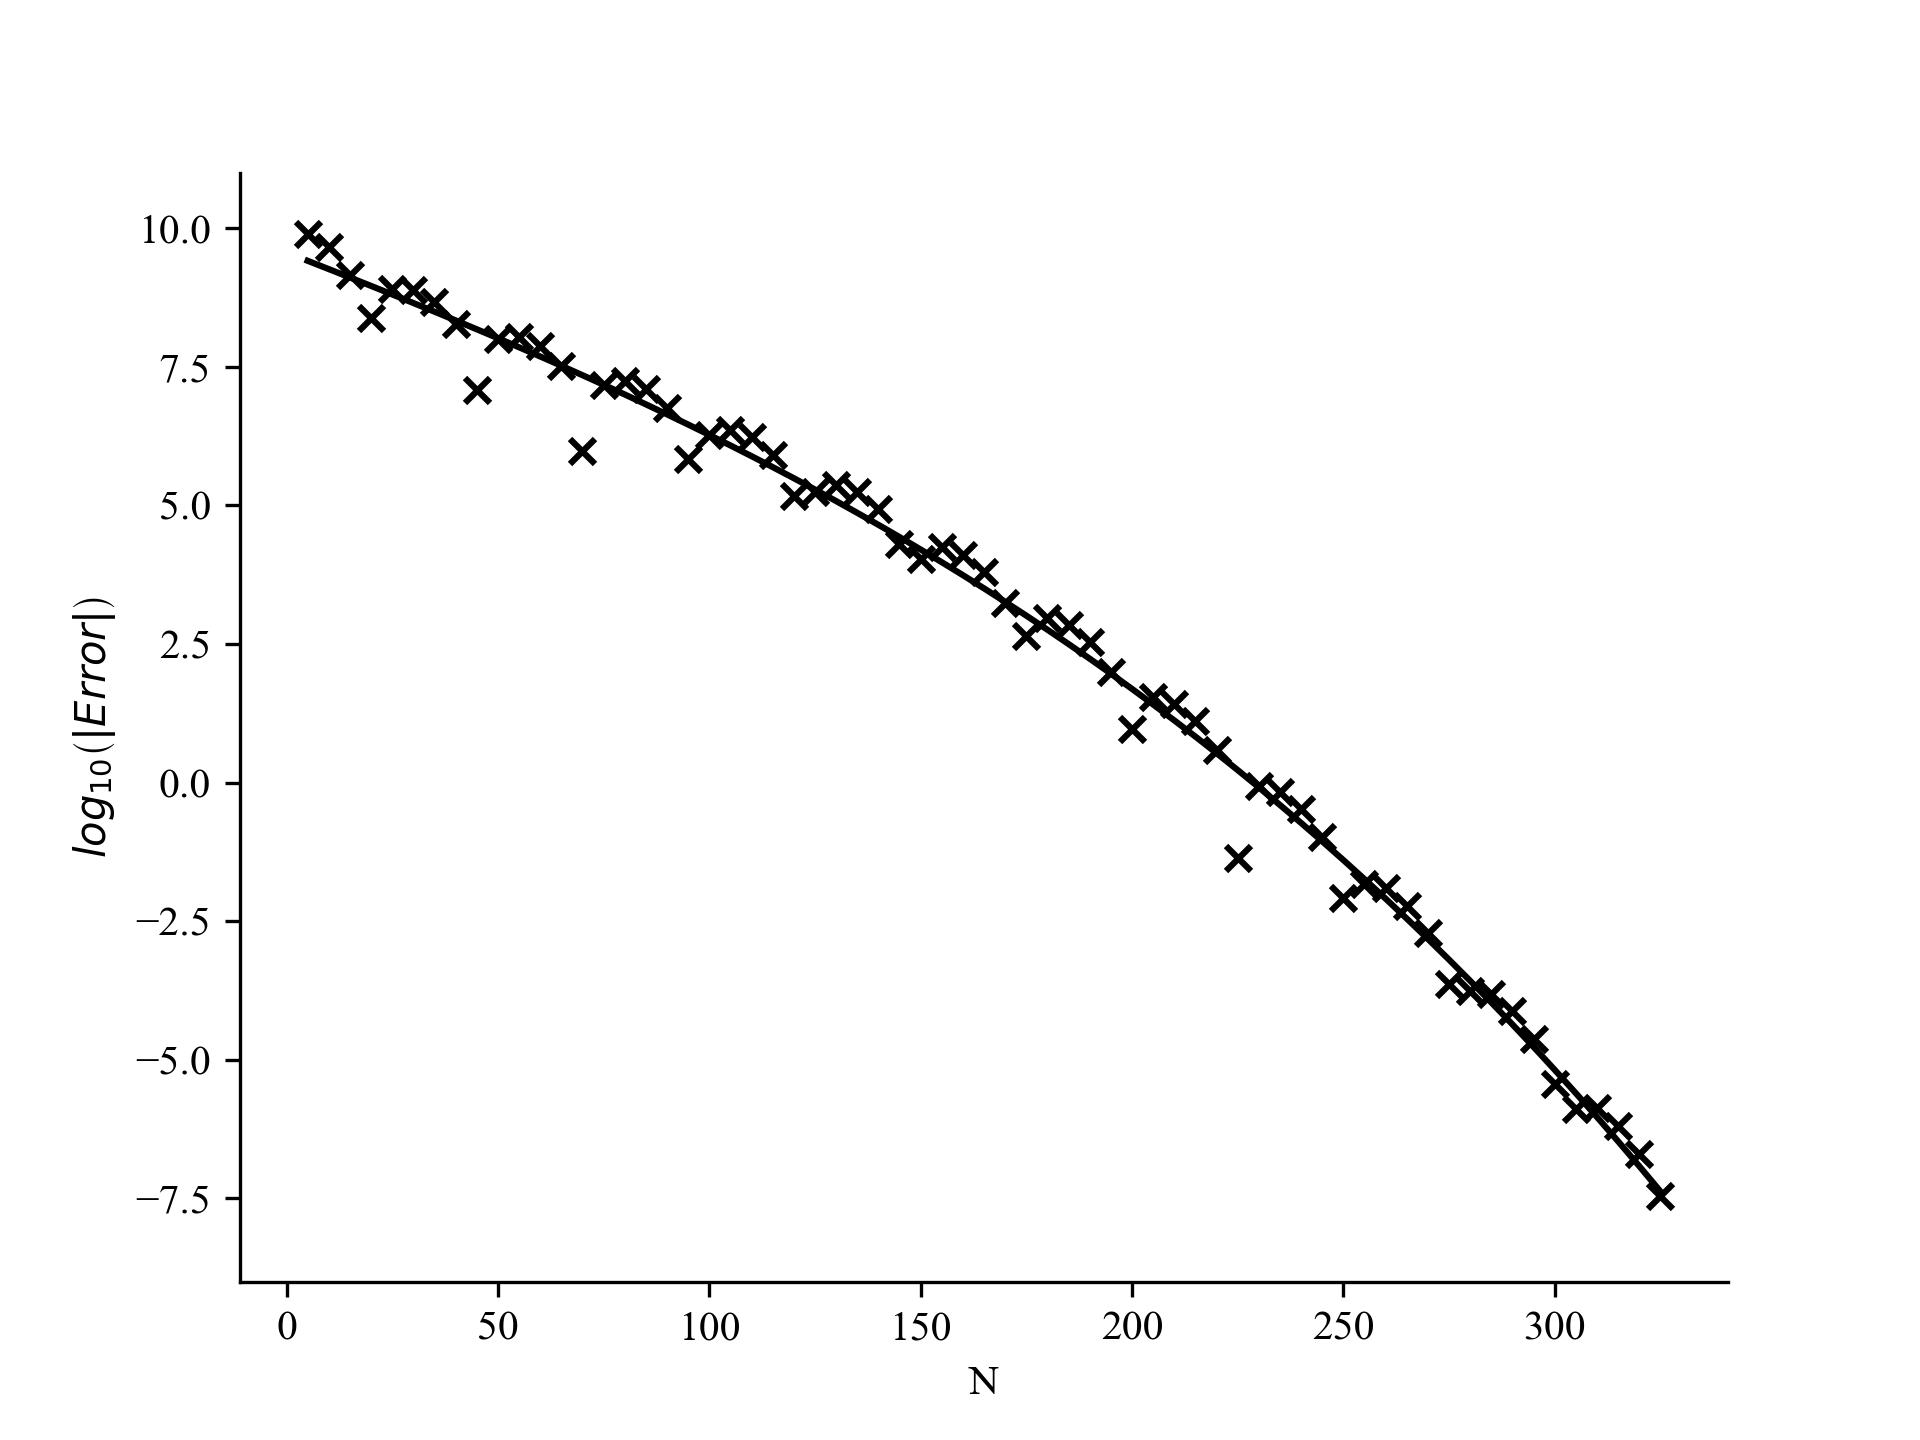
\includegraphics[width=0.8\linewidth]{error-plot-KJD-rightup.jpg}
    \caption[\emph{DJD-Up: The speed of error convergence.}]{\emph{DJD-Up: The speed of error convergence.} \textbf{Note}: reference value $=18.125462041$, criteria of negligible error from the product of payoff function and density is $10^{-15}$, $R^2=0.993$, and the regression line is $log_{10}\left(|Error|\right) = -8.375\times 10^{-6}N^2-0.0304N+9.9522$.}

    \label{fig:label}
\end{figure}


\subsection{Stochastic Volatility Jump Model}
\begin{figure}[H]
    \centering
    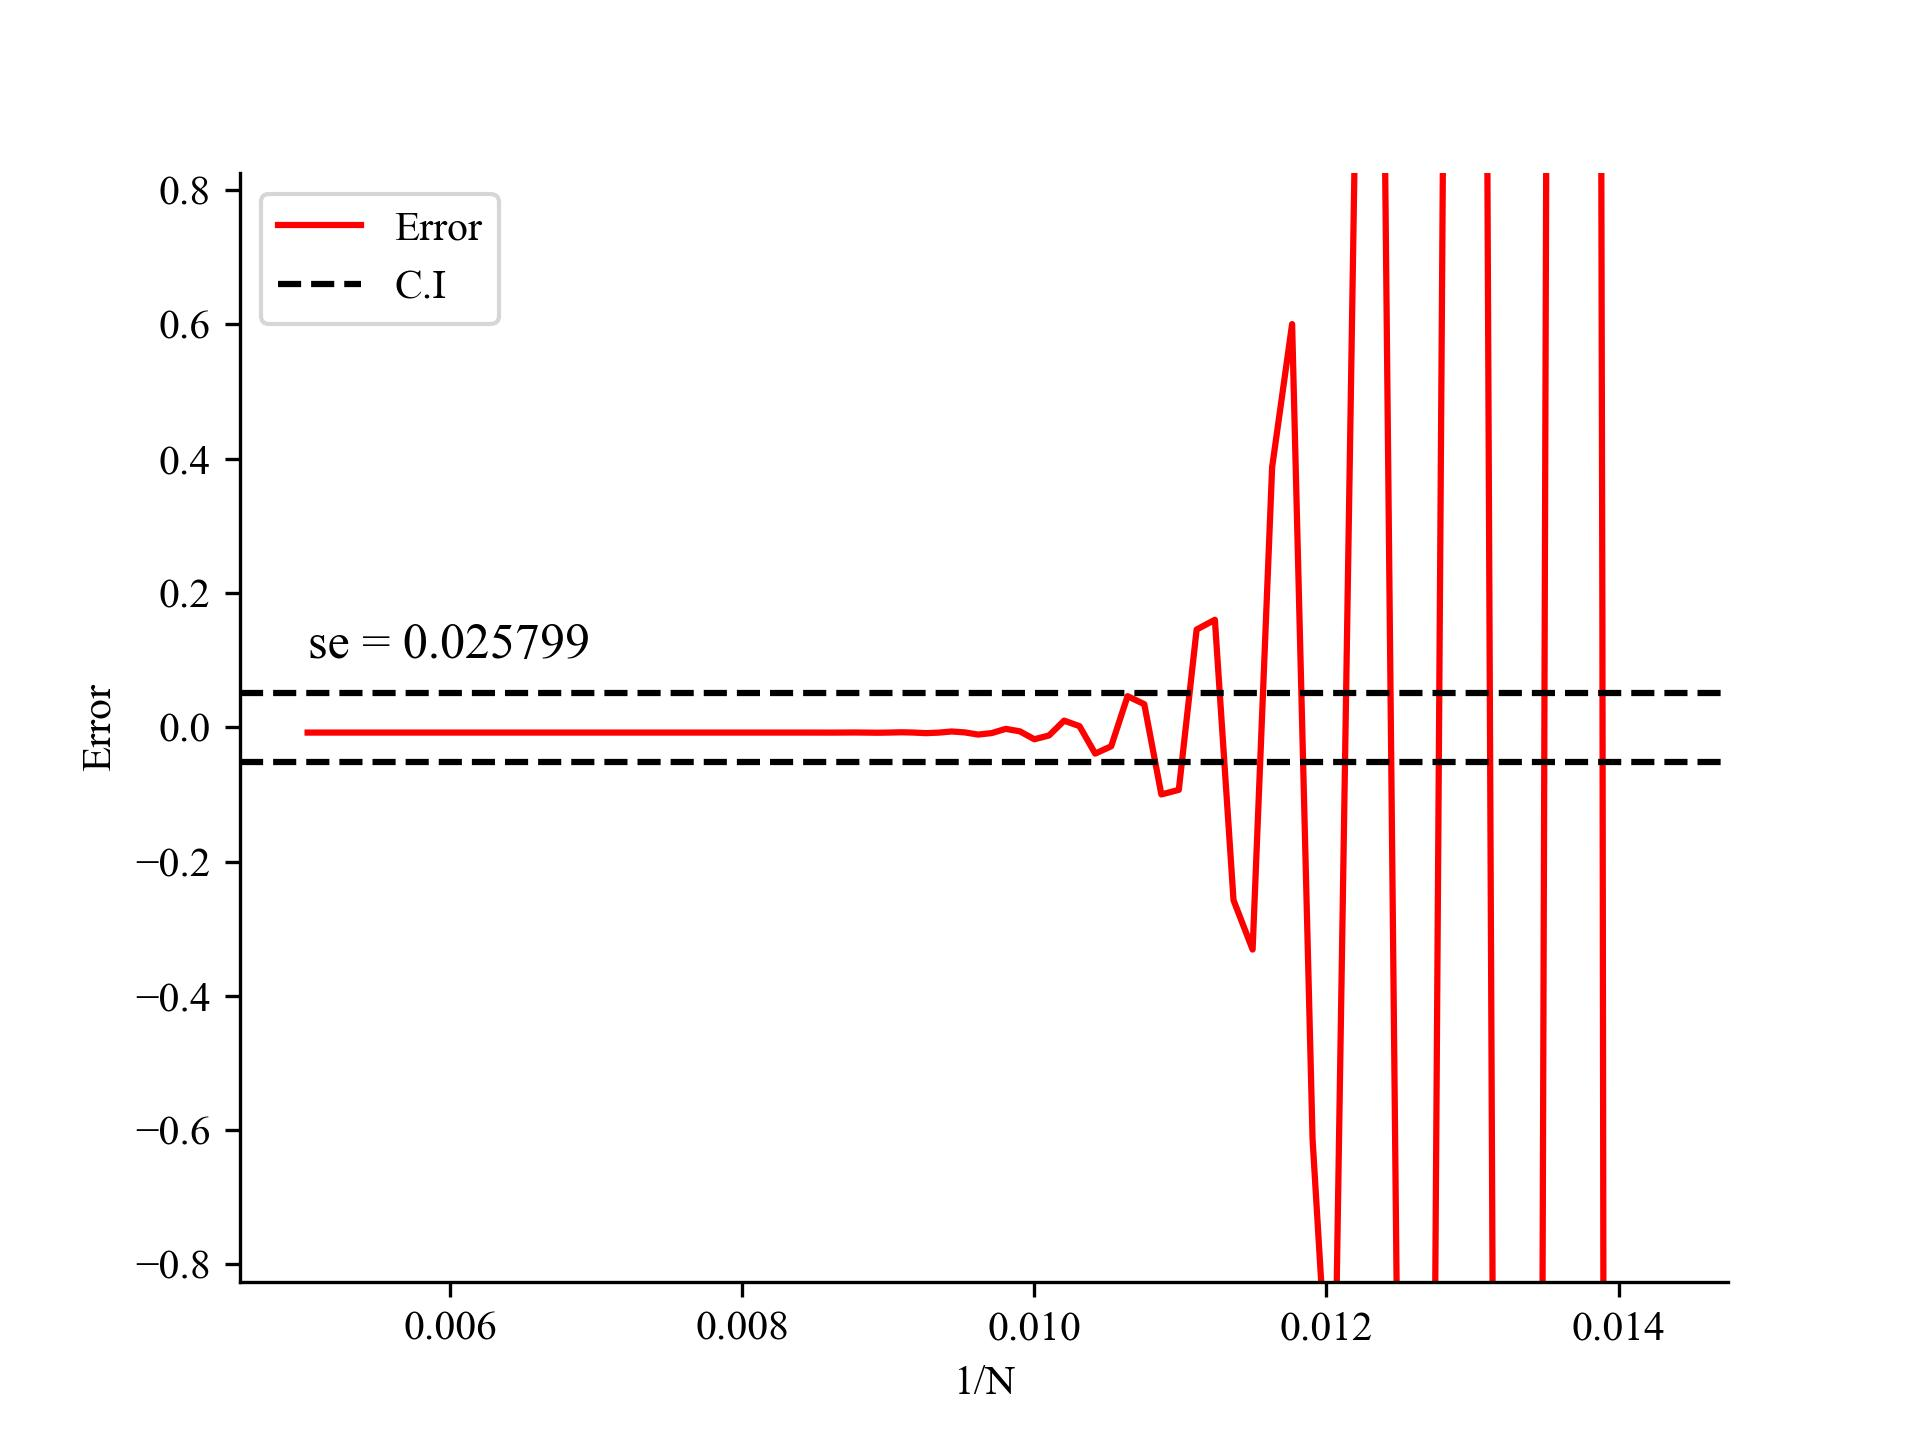
\includegraphics[width=0.8\linewidth]{value-plot-SVJ-rightup.jpg}
    \caption[\emph{SVJ-Up: Value accuracy comparing to the simulation with} $10^7$ \emph{paths.}]{\emph{SVJ-Up: Value accuracy comparing to the simulation with} $10^7$ \emph{paths.} \textbf{Note}: mean value from simulation = 31.12008, criteria of negligible error from the product of payoff function and density is $10^{-6}$, and $N$ starts from $10$  with increment $=2$.}

    \label{fig:label}
\end{figure}
\begin{figure}[H]
    \centering
    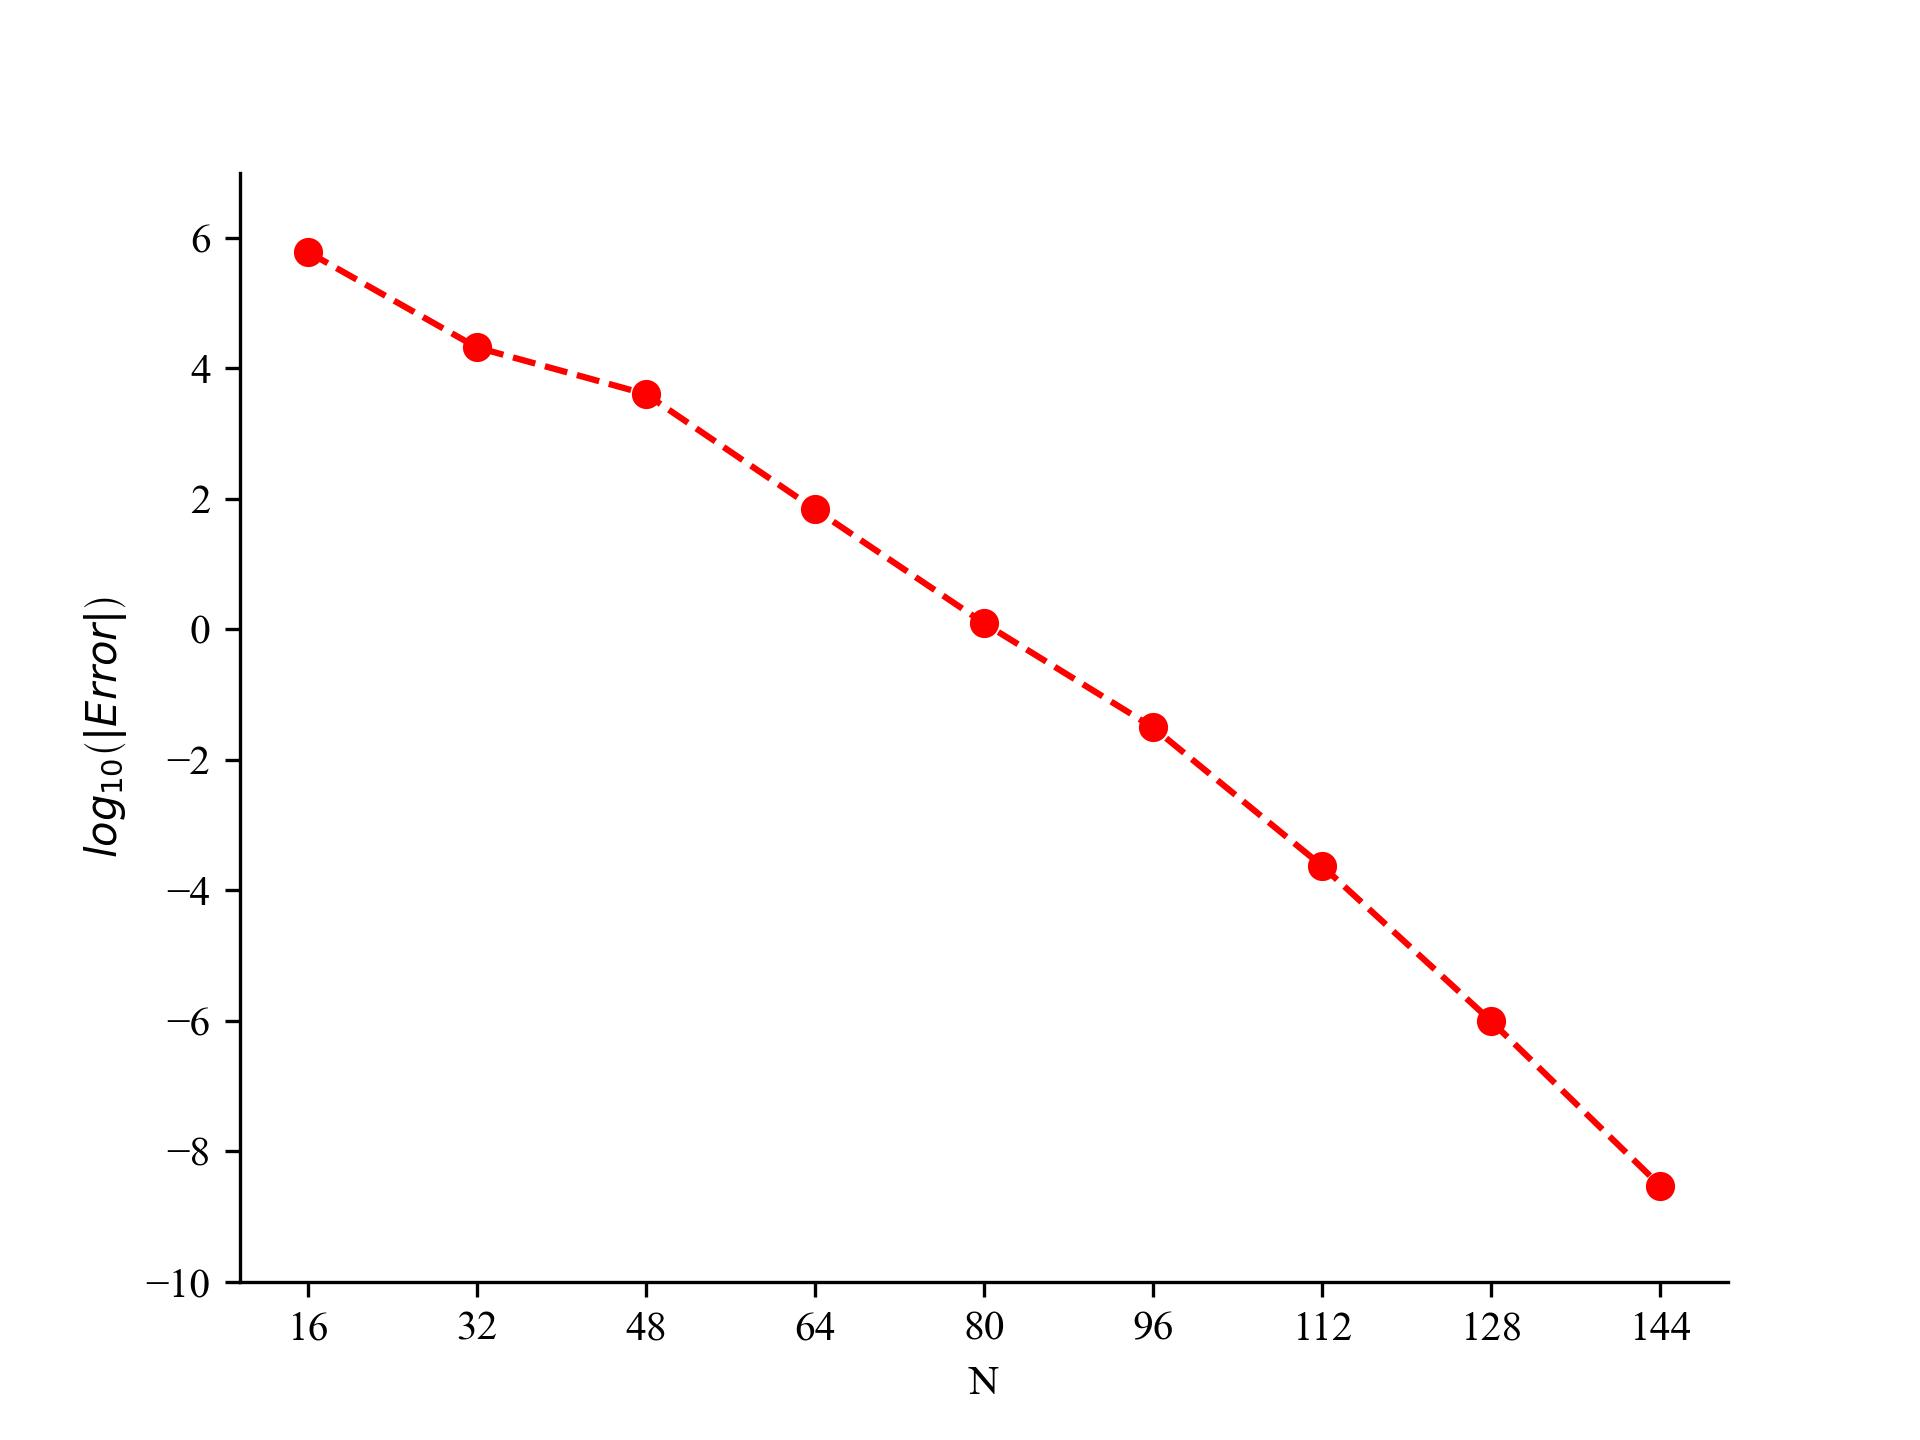
\includegraphics[width=0.8\linewidth]{error-plot-SVJ-rightup.jpg}
    \caption[\emph{SVJ-Up: The speed of error convergence.}]{\emph{SVJ-Up: The speed of error convergence.} \textbf{Note}: reference value $=31.1121085763$, criteria of negligible error from the product of payoff function and density is $10^{-15}$, $R^2=0.993$, and the regression line is $log_{10}\left(|Error|\right) = -0.0004N^2-0.0352N+9.6743$.}
    
    \label{fig:label}
\end{figure}


\subsection{Normal Inverse Gaussian Model}
\begin{figure}[H]
    \centering
    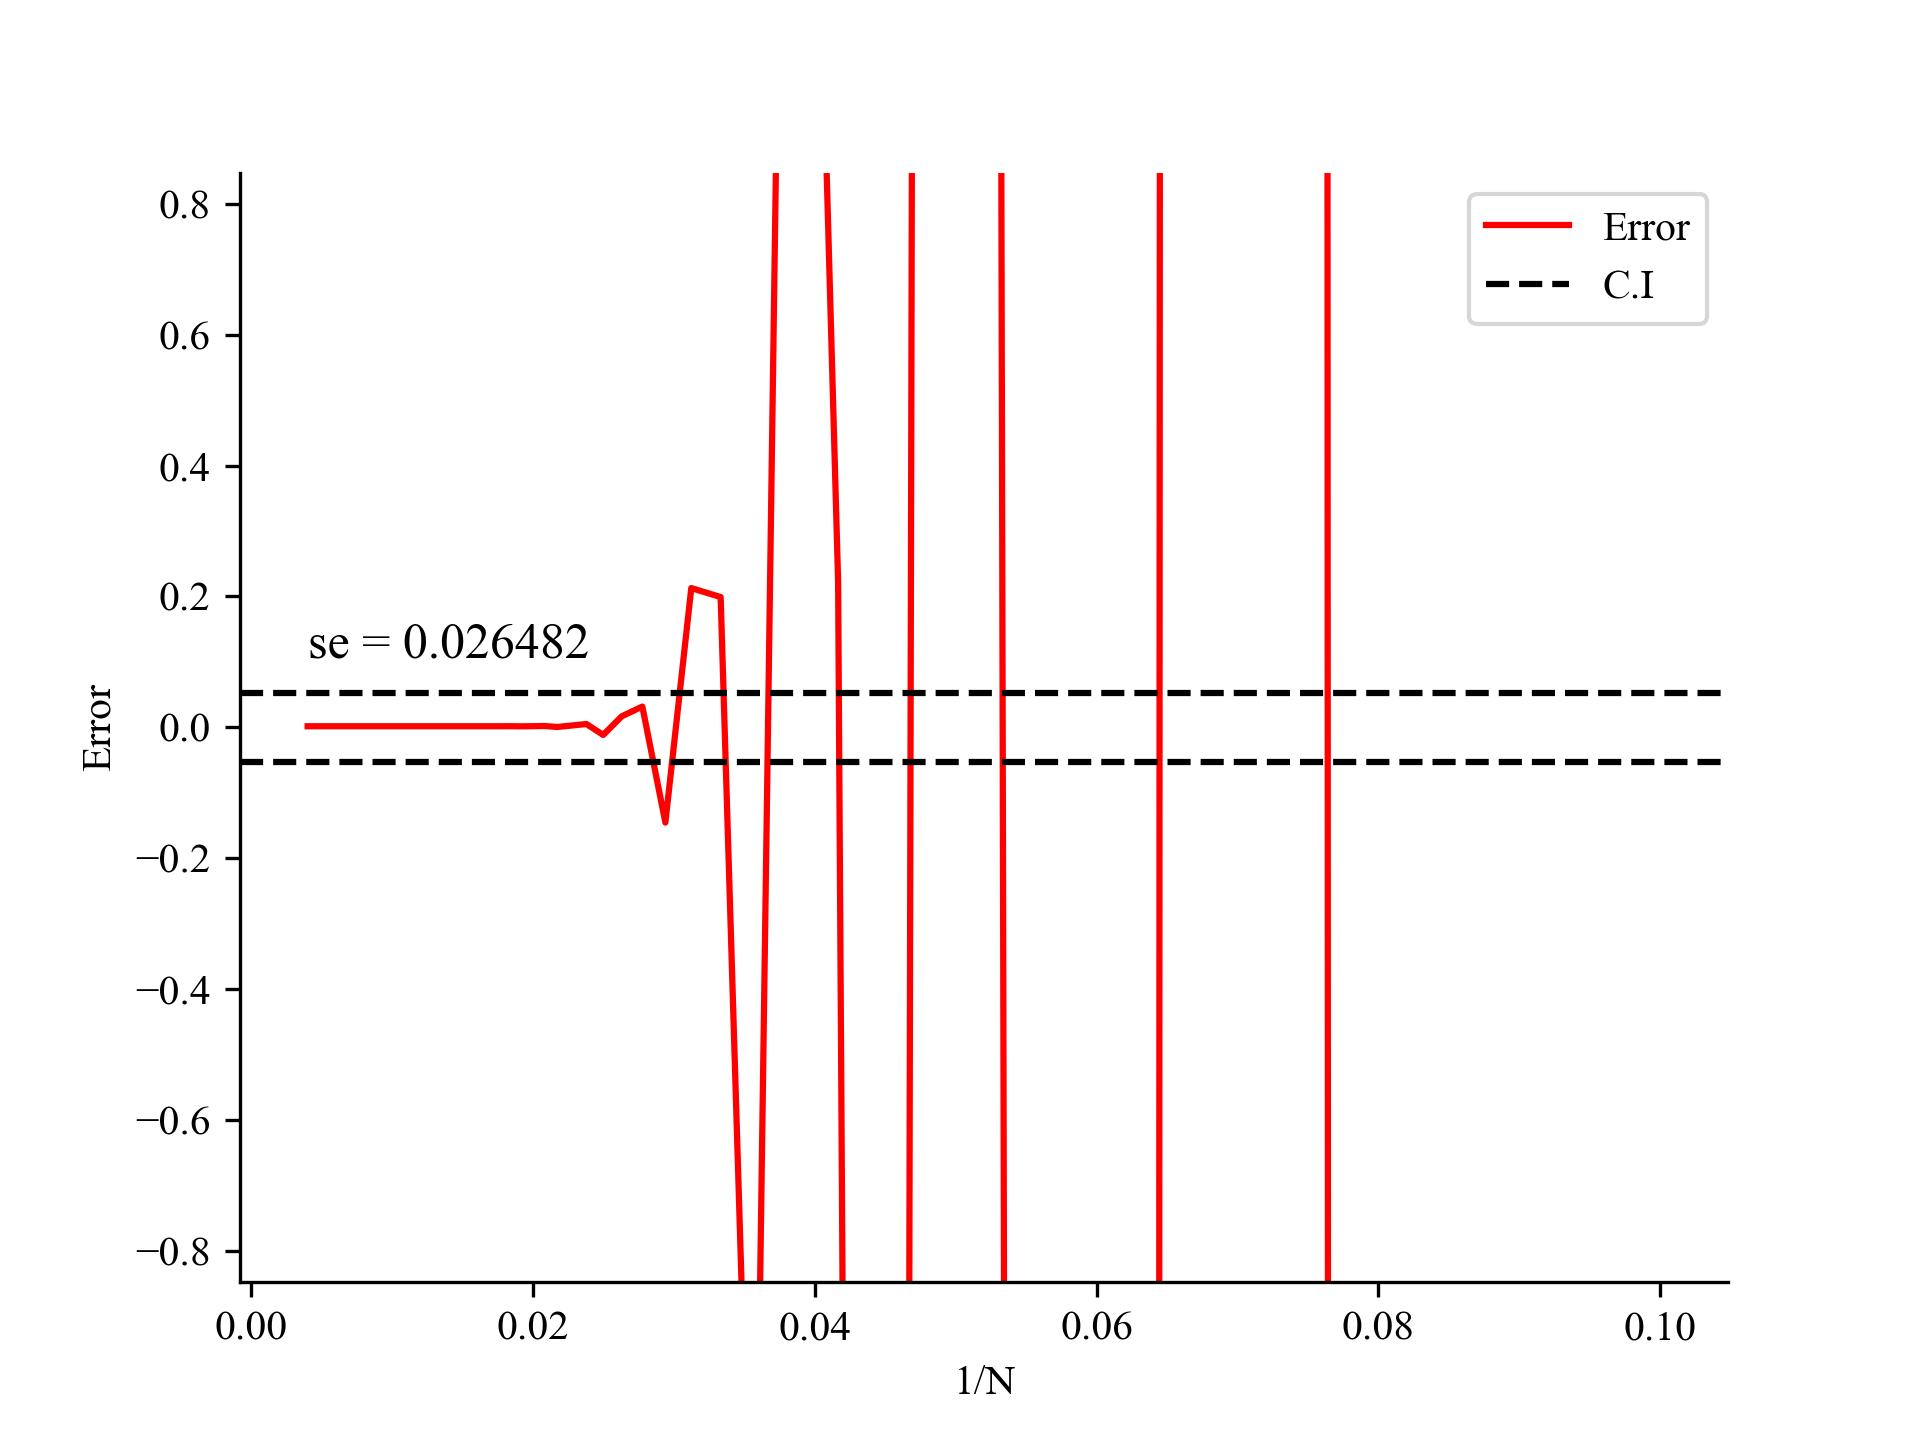
\includegraphics[width=0.8\linewidth]{value-plot-NIG-rightup.jpg}
    \caption[\emph{NIG-Up: Value accuracy comparing to the simulation with} $10^7$ \emph{paths.}]{\emph{NIG-Up: Value accuracy comparing to the simulation with} $10^7$ \emph{paths.} \textbf{Note}: mean value from simulation = 28.317193, criteria of negligible error from the product of payoff function and density is $10^{-6}$, and $N$ starts from $10$  with increment $=2$.}
 
    \label{fig:label}
\end{figure}

\begin{figure}[H]
    \centering
    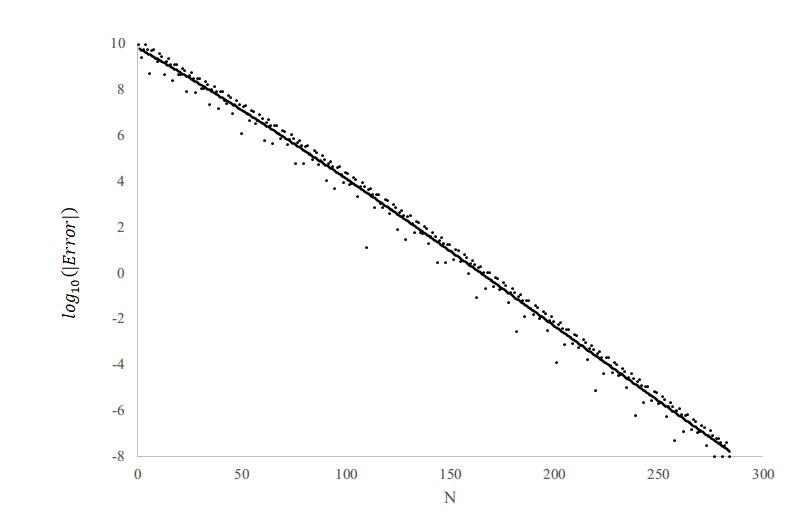
\includegraphics[width=0.8\linewidth]{error-plot-NIG-rightup.jpg}
    \caption[\emph{NIG-Up: The speed of error convergence.}]{\emph{NIG-Up: The speed of error convergence.} \textbf{Note}: reference value $=28.3185901456$, criteria of negligible error from the product of payoff function and density is $10^{-15}$, $R^2=0.991$, and the regression line is $log_{10}\left(|Error|\right) = -7.502\times 10^{-5}N^2-0.0508N+9.8393$.}

    \label{fig:label}
\end{figure}


\subsection{Variance Gamma Model}
\begin{figure}[H]
    \centering
    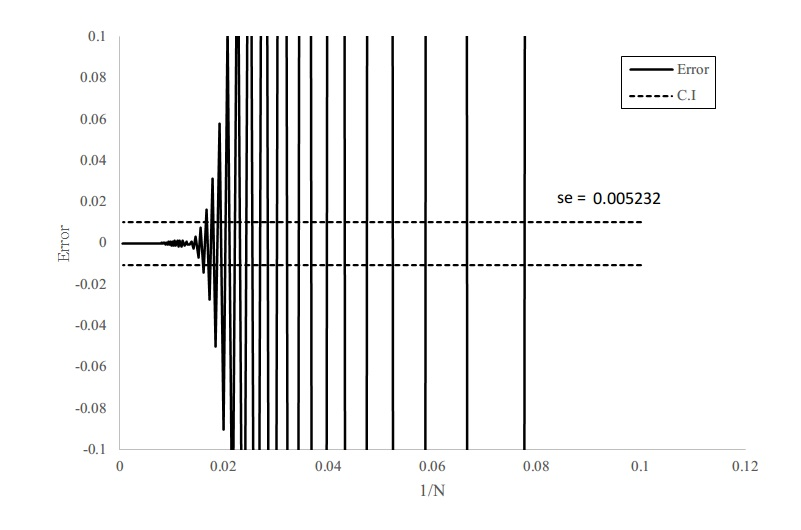
\includegraphics[width=0.8\linewidth]{value-plot-VG-rightup.jpg}
    \caption[\emph{VG-Up: Value accuracy comparing to the simulation with} $10^7$ \emph{paths.}]{\emph{VG-Up: Value accuracy comparing to the simulation with} $10^7$ \emph{paths.} \textbf{Note}: mean value from simulation = 8.219291, criteria of negligible error from the product of payoff function and density is $10^{-6}$, and $N$ starts from $10$  with increment $=2$.}

    \label{fig:label}
\end{figure}

\begin{figure}[H]
    \centering
    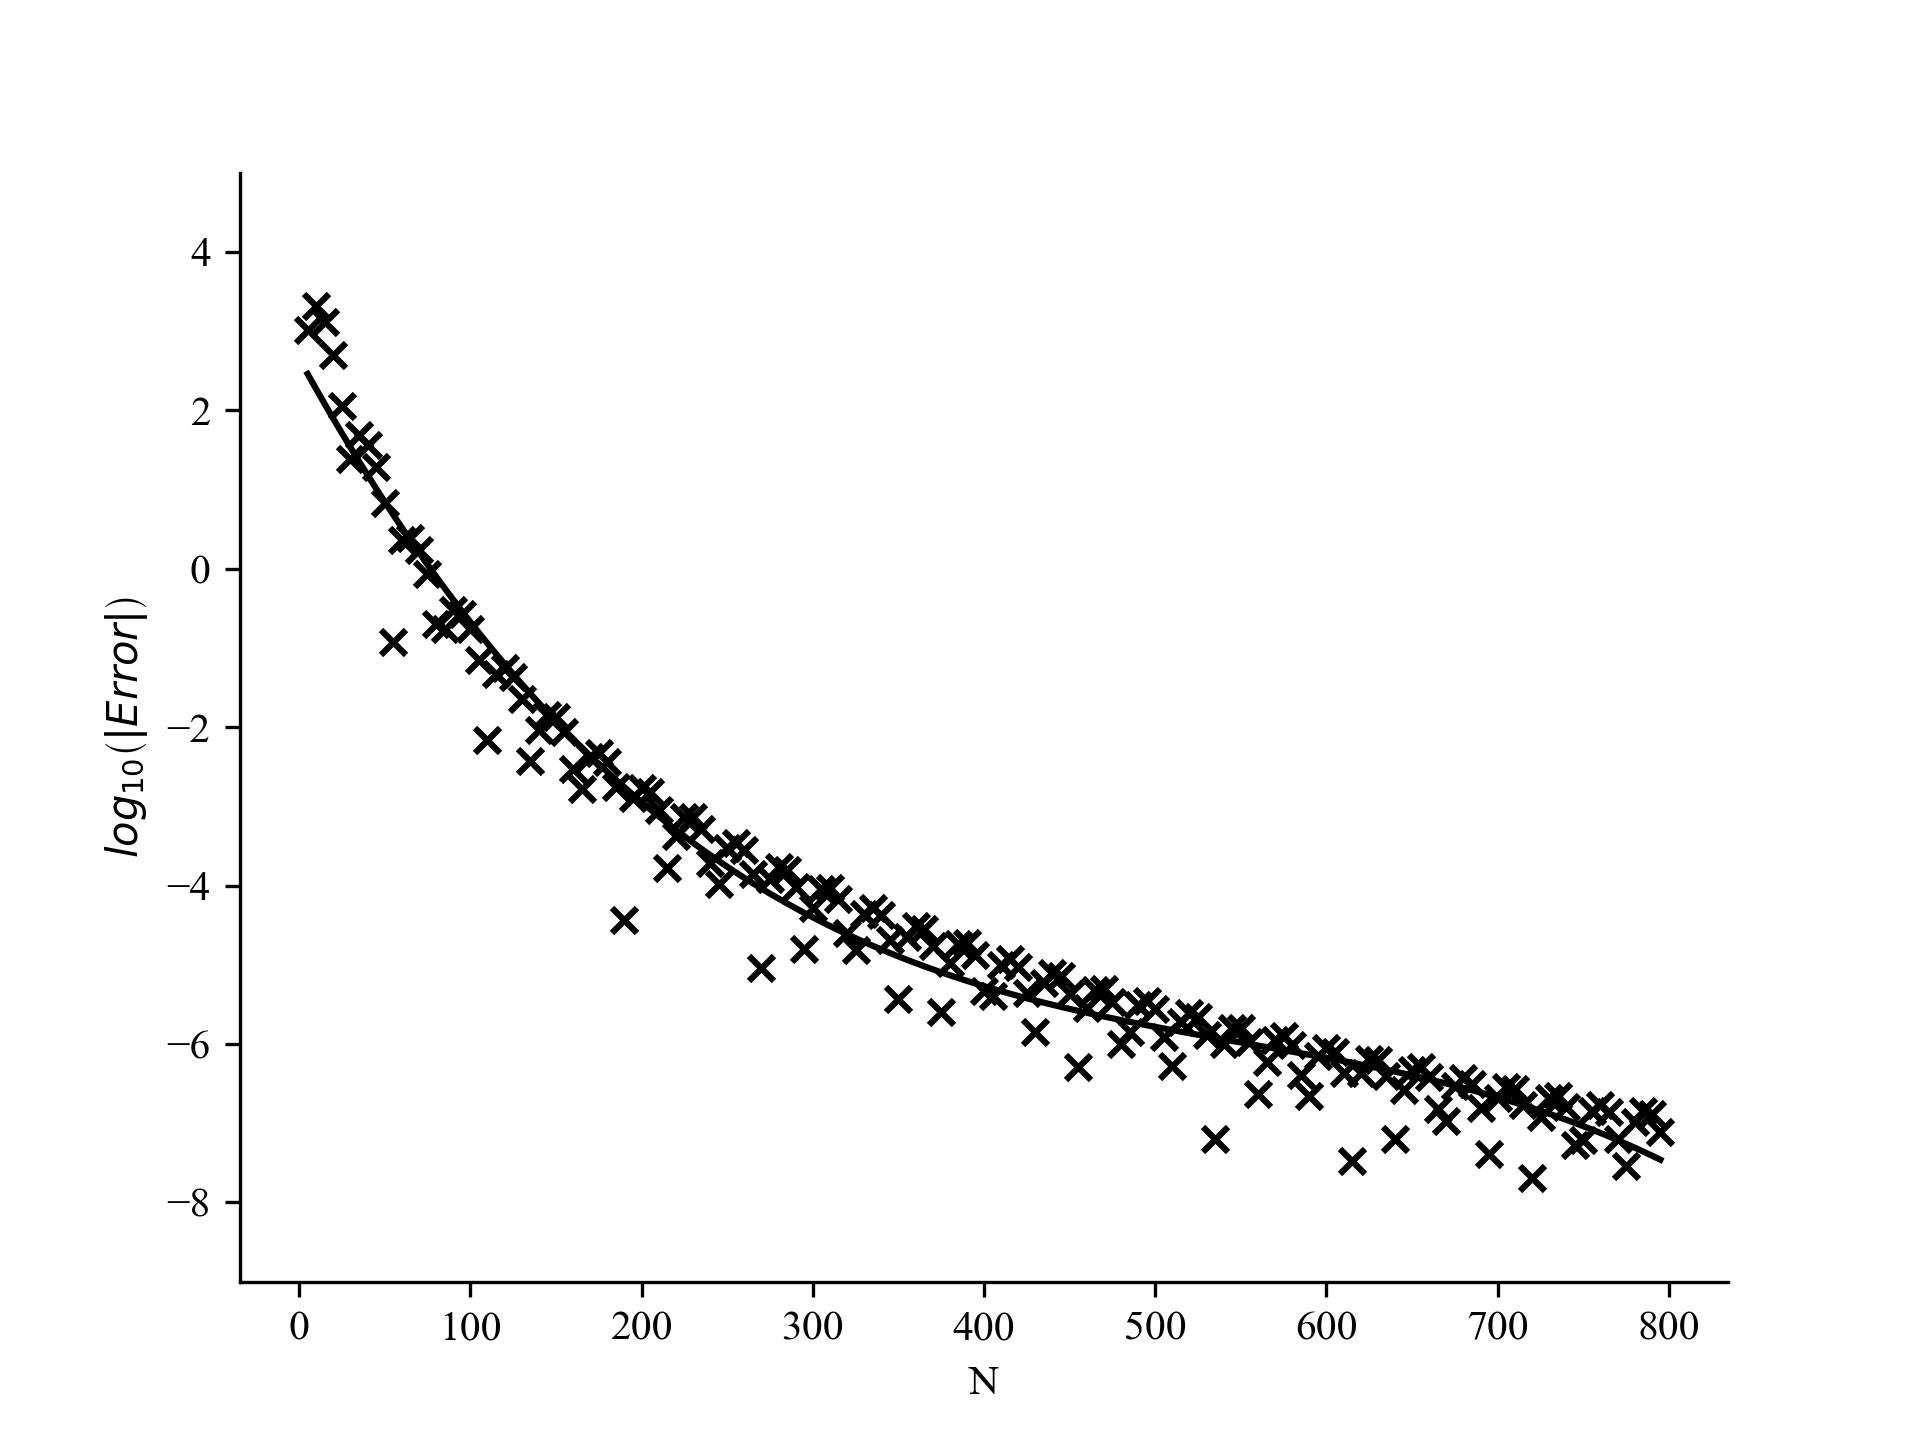
\includegraphics[width=0.8\linewidth]{error-plot-VG-rightup.jpg}
    \caption[\emph{VG-Up: The speed of error convergence.}]{\emph{VG-Up: The speed of error convergence.} \textbf{Note}: reference value $=8.219228342$, criteria of negligible error from the product of payoff function and density is $10^{-15}$, $R^2=0.972$, and the regression line is $log_{10}\left(|Error|\right) = 0.0001N^2-0.0535N+3.3449$.}

    \label{fig:label}
\end{figure}

\begin{figure}[ht]
    \begin{table}[H]
      \centering
      \caption[$log_{10}(|Error|)=AN^2+BN+C$]{Right Up - $log_{10}(|Error|)=AN^2+BN+C$}
    \end{table}
    \centering
        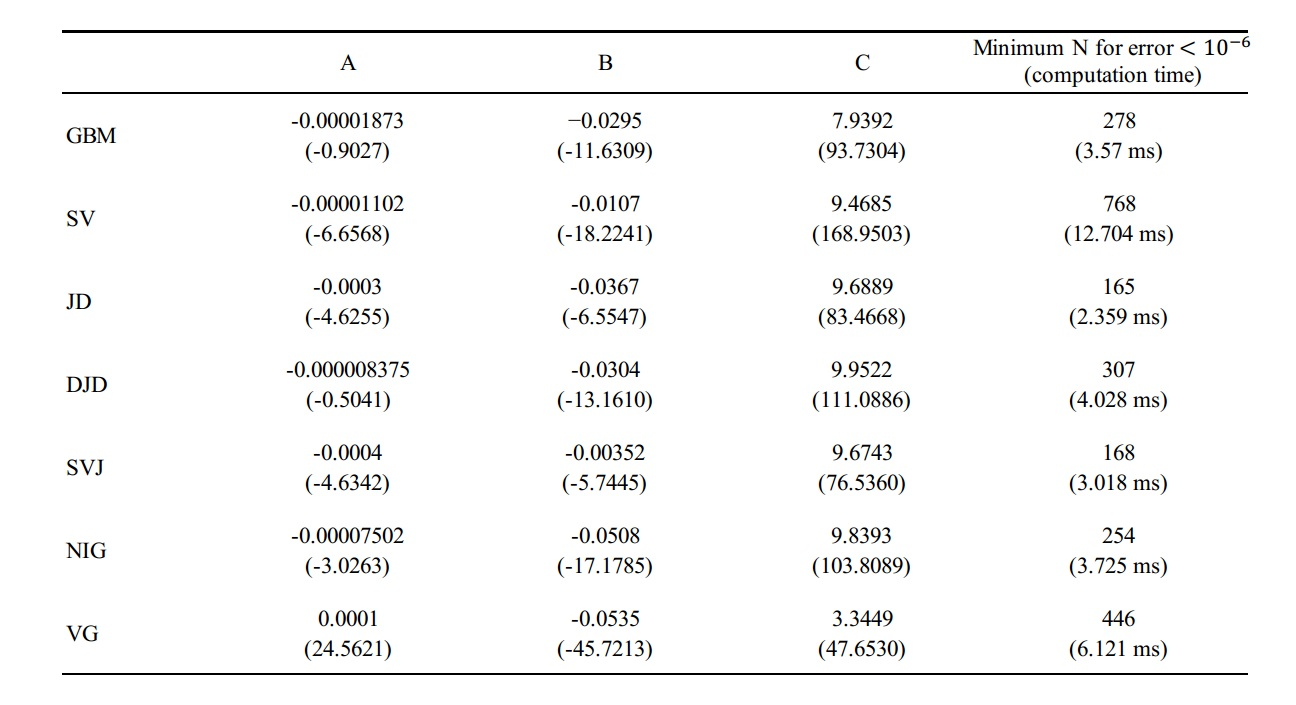
\includegraphics[width=1.1\textwidth,center]{rightup-table.jpg}
    \caption*{\small{This table reports the coefficients of the regression and t-statistics shown inside the parentheses in accordance with the coefficient. The time measurements in the final column are expressed in milliseconds and pertain to the MacBook Air equipped with the Apple M1 chip.}}
\end{figure}

Table 3.2 shows results that are very similar to those in Table 3.1. However, compared to the call option, the linear term becomes smaller and the quadratic term becomes more significant. This is because the payoff function grows faster compared to the call option, requiring a larger $N$ to achieve error convergence. Therefore, the significant negative coefficient of the quadratic term indicates slower error convergence initially, followed by faster error convergence. It can be observed that achieving an error below $10^{-6}$ requires a larger $N$. Additionally, the value of quadratic terms are still small. Although $N$ has increased, the computation time has not significantly increased, indicating that this model maintains a linear time complexity. Additionally, even for the stochastic volatility model with the highest $N$, it only requires 0.012 milliseconds to complete the calculation.



\section{Concave Payoff for the Right End}
In the other category of polynomial options, we discuss the payoff function of a polynomial option where the leading coefficient is negative. Because the polynomial has a negative leading coefficient, the curve on the far right side must be concave. For this payoff function, as the stock price approaches infinity, the payoff will always be zero. I call this category "Right Down".
To examine this polynomial option, the setting is $A(S_T)=-0.0031S_T^4+0.2358S_T^3-5.4793S_T^2+39.474S_T-44.235$ which is a high order polynomial function and with randomly chosen coefficients. Then, the roots of $A(S_T)$ is $1.363962$, $10.620047$, $25.599102$ and $38.481405$. As a result, the array of the positive intervals that can be obtained with $\left[0, \, 1.363962,\right]$, $ \left[10.620047, \, 25.599102\right]$, $\left[ 38.481405, \,\infty \right]$. All the following experiments are under $S_0=30$.

Note that the reference values for analyzing error convergence are calculated using binomial tree only for geometric Brownian motion. For other stochastic processes, these values are calculated under this model with $N=10^5$, because there are no analytical solutions or tree-based methods for pricing polynomial options aside from geometric Brownian motion. These values fall within the confidence interval constructed by simulating $10^7$ paths within two standard errors. 
\newpage

\subsection{Geometric Brownian Motion}
\begin{figure}[H]
    \centering
    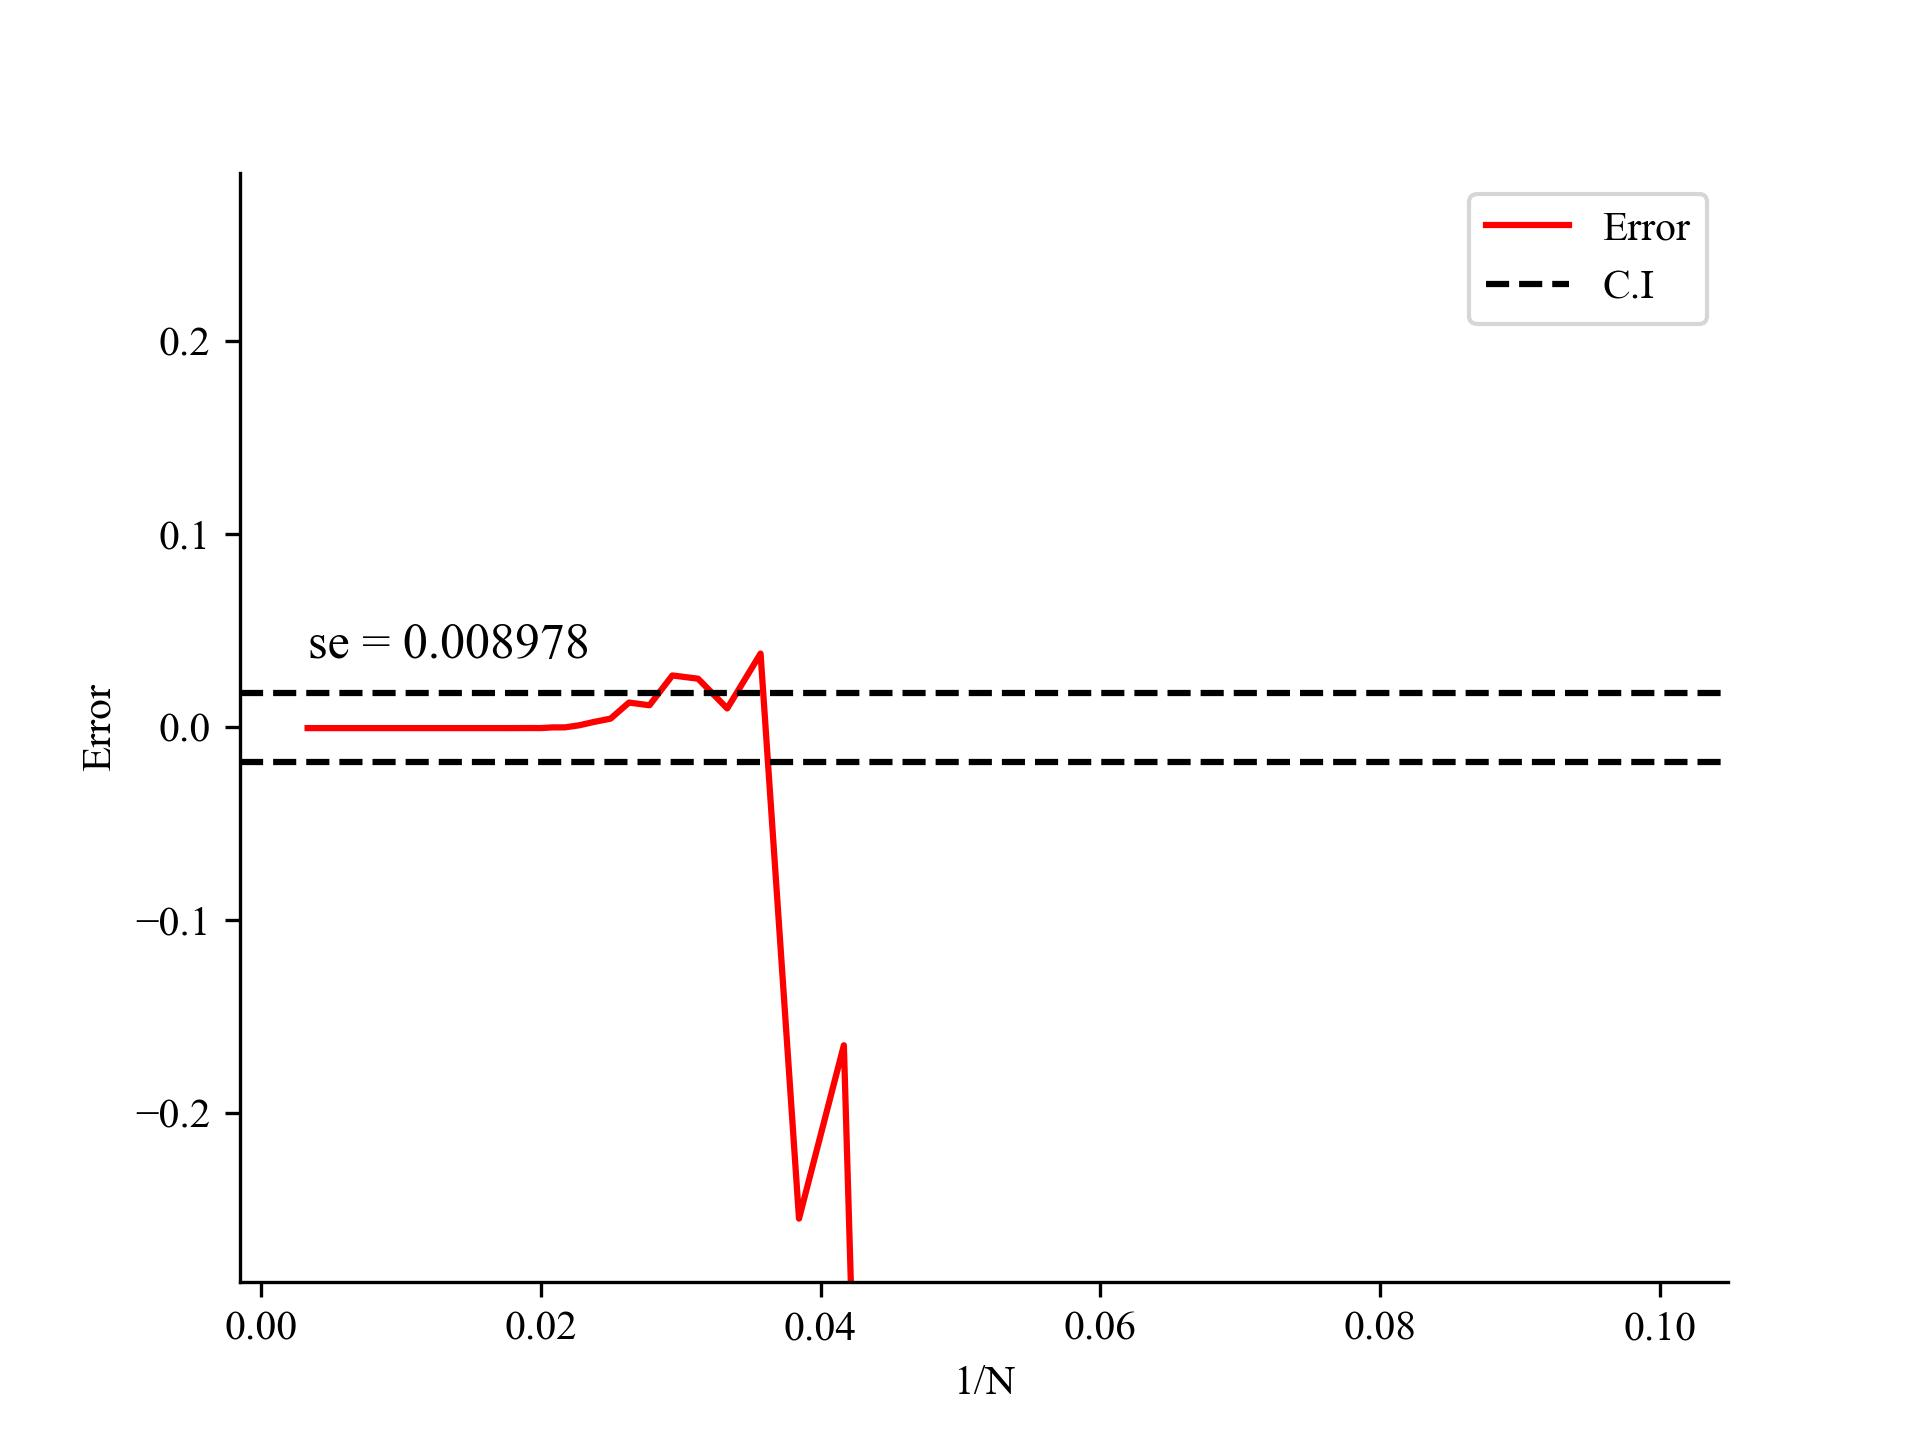
\includegraphics[width=0.8\linewidth]{value-plot-GBM-bothdown.jpg}
    \caption[\emph{GBM-Down: Value accuracy comparing to the simulation with} $10^7$ \emph{paths.}]{\emph{GBM-Down: Value accuracy comparing to the simulation with} $10^7$ \emph{paths.} \textbf{Note}: mean value from simulation = 48.755816, criteria of negligible error from the product of payoff function and density is $10^{-6}$, and $N$ starts from $10$  with increment $=2$.}
  
    \label{fig:label}
\end{figure}

\begin{figure}[H]
    \centering
    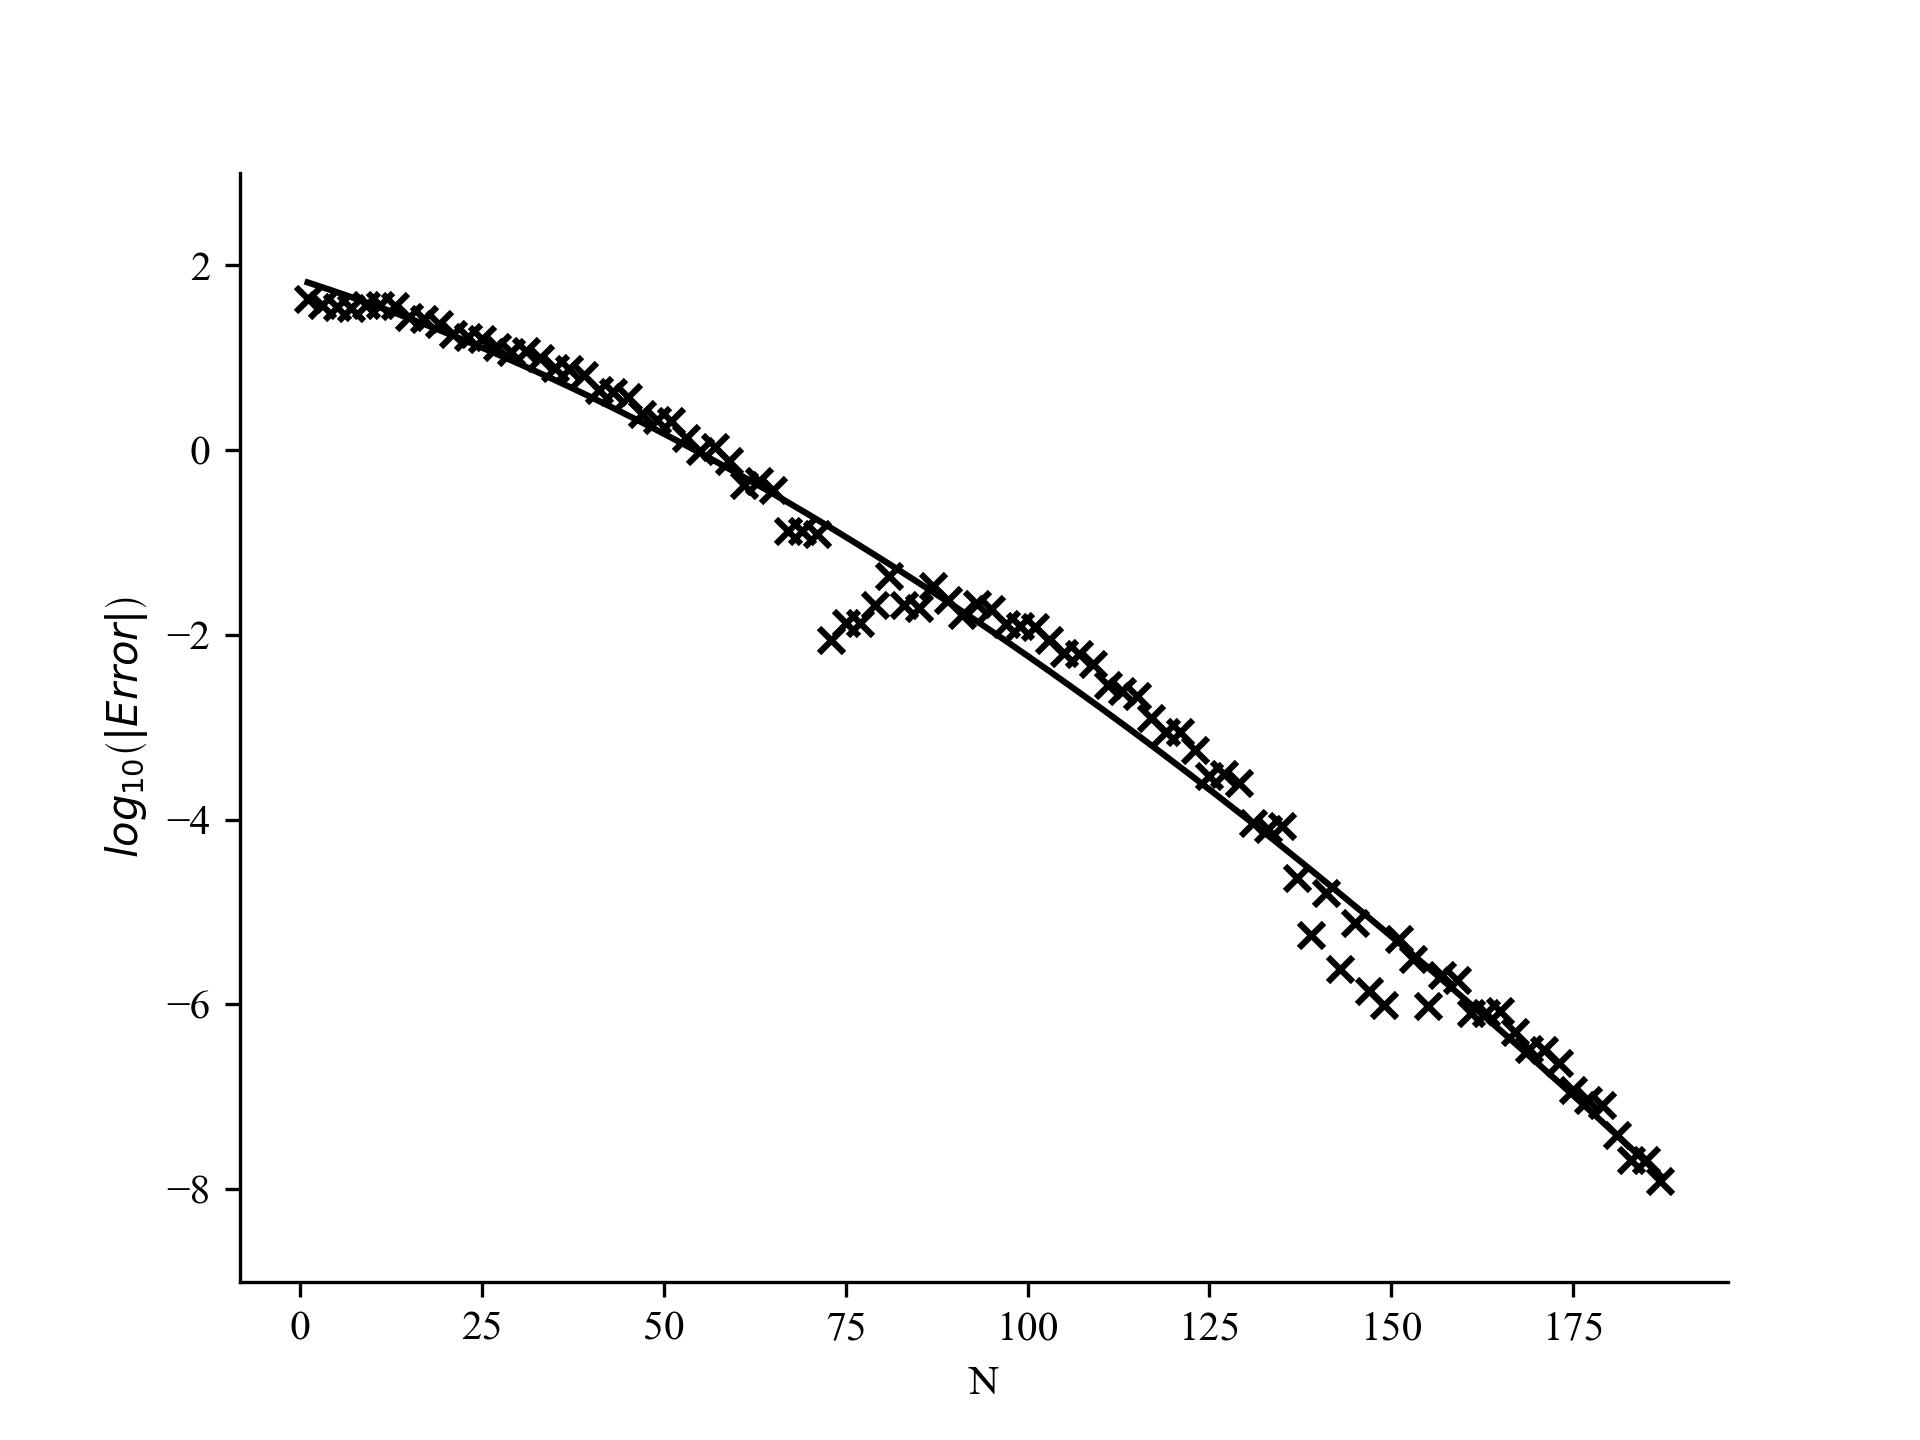
\includegraphics[width=0.8\linewidth]{error-plot-GBM-bothdown.jpg}
    \caption[\emph{GBM-Down: The speed of error convergence.}]{\emph{GBM-Down: The speed of error convergence.} \textbf{Note}: reference value $=48.7553402894$, criteria of negligible error from the product of payoff function and density is $10^{-15}$, $R^2=0.992$, and the regression line is $log_{10}\left(|Error|\right) = -0.0002N^2-0.0251N+1.8391$.}

    \label{fig:label}
\end{figure}


\subsection{Stochastic Volatility Model}
\begin{figure}[H]
    \centering
    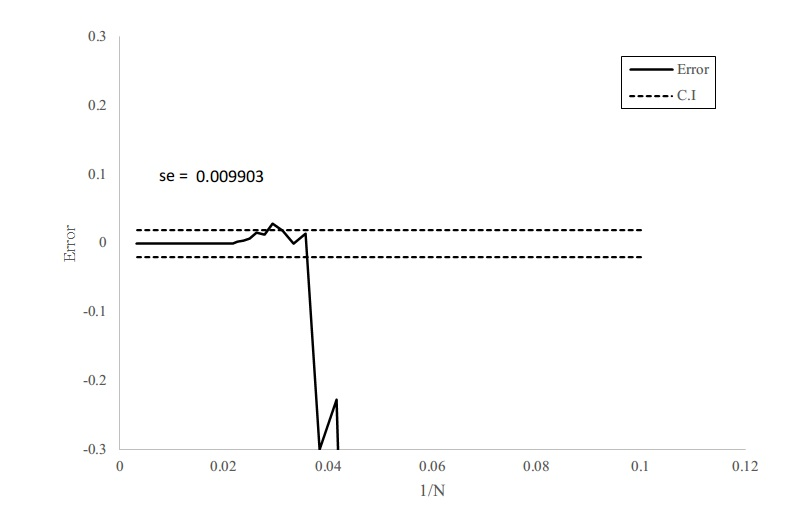
\includegraphics[width=0.8\linewidth]{value-plot-Heston-bothdown.jpg}
    \caption[\emph{SV-Down: Value accuracy comparing to the simulation with} $10^7$ \emph{paths.}]{\emph{SV-Down: Value accuracy comparing to the simulation with} $10^7$ \emph{paths.} \textbf{Note}: mean value from simulation = 49.003536, criteria of negligible error from the product of payoff function and density is $10^{-6}$, and $N$ starts from $10$  with increment $=2$.}

    \label{fig:label}
\end{figure}
\begin{figure}[H]
    \centering
    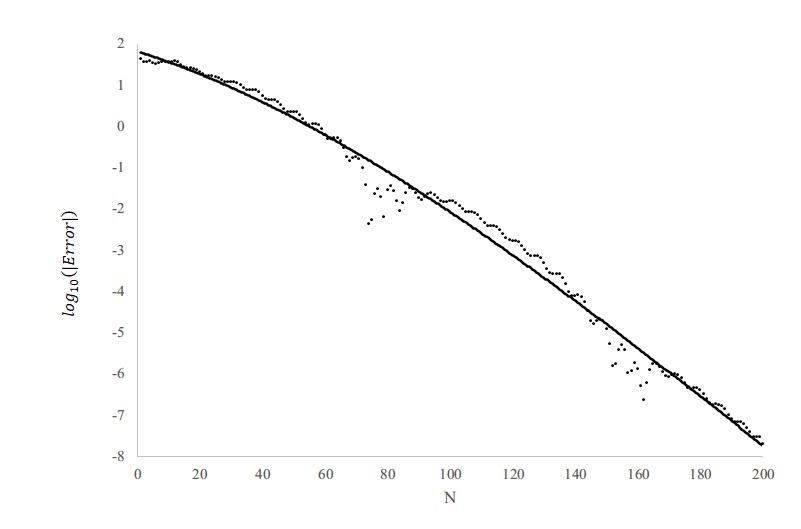
\includegraphics[width=0.8\linewidth]{error-plot-Heston-bothdown.jpg}
    \caption[\emph{SV-Down: The speed of error convergence.}]{\emph{SV-Down: The speed of error convergence.} \textbf{Note}: reference value $=49.0026564304$, criteria of negligible error from the product of payoff function and density is $10^{-15}$, $R^2=0.988$, and the regression line is $log_{10}\left(|Error|\right) = -0.0002N^2-0.0241N+1.8224$.}

    \label{fig:label}
\end{figure}


\subsection{Log-normal Jump Diffusion Model}
\begin{figure}[H]
    \centering
    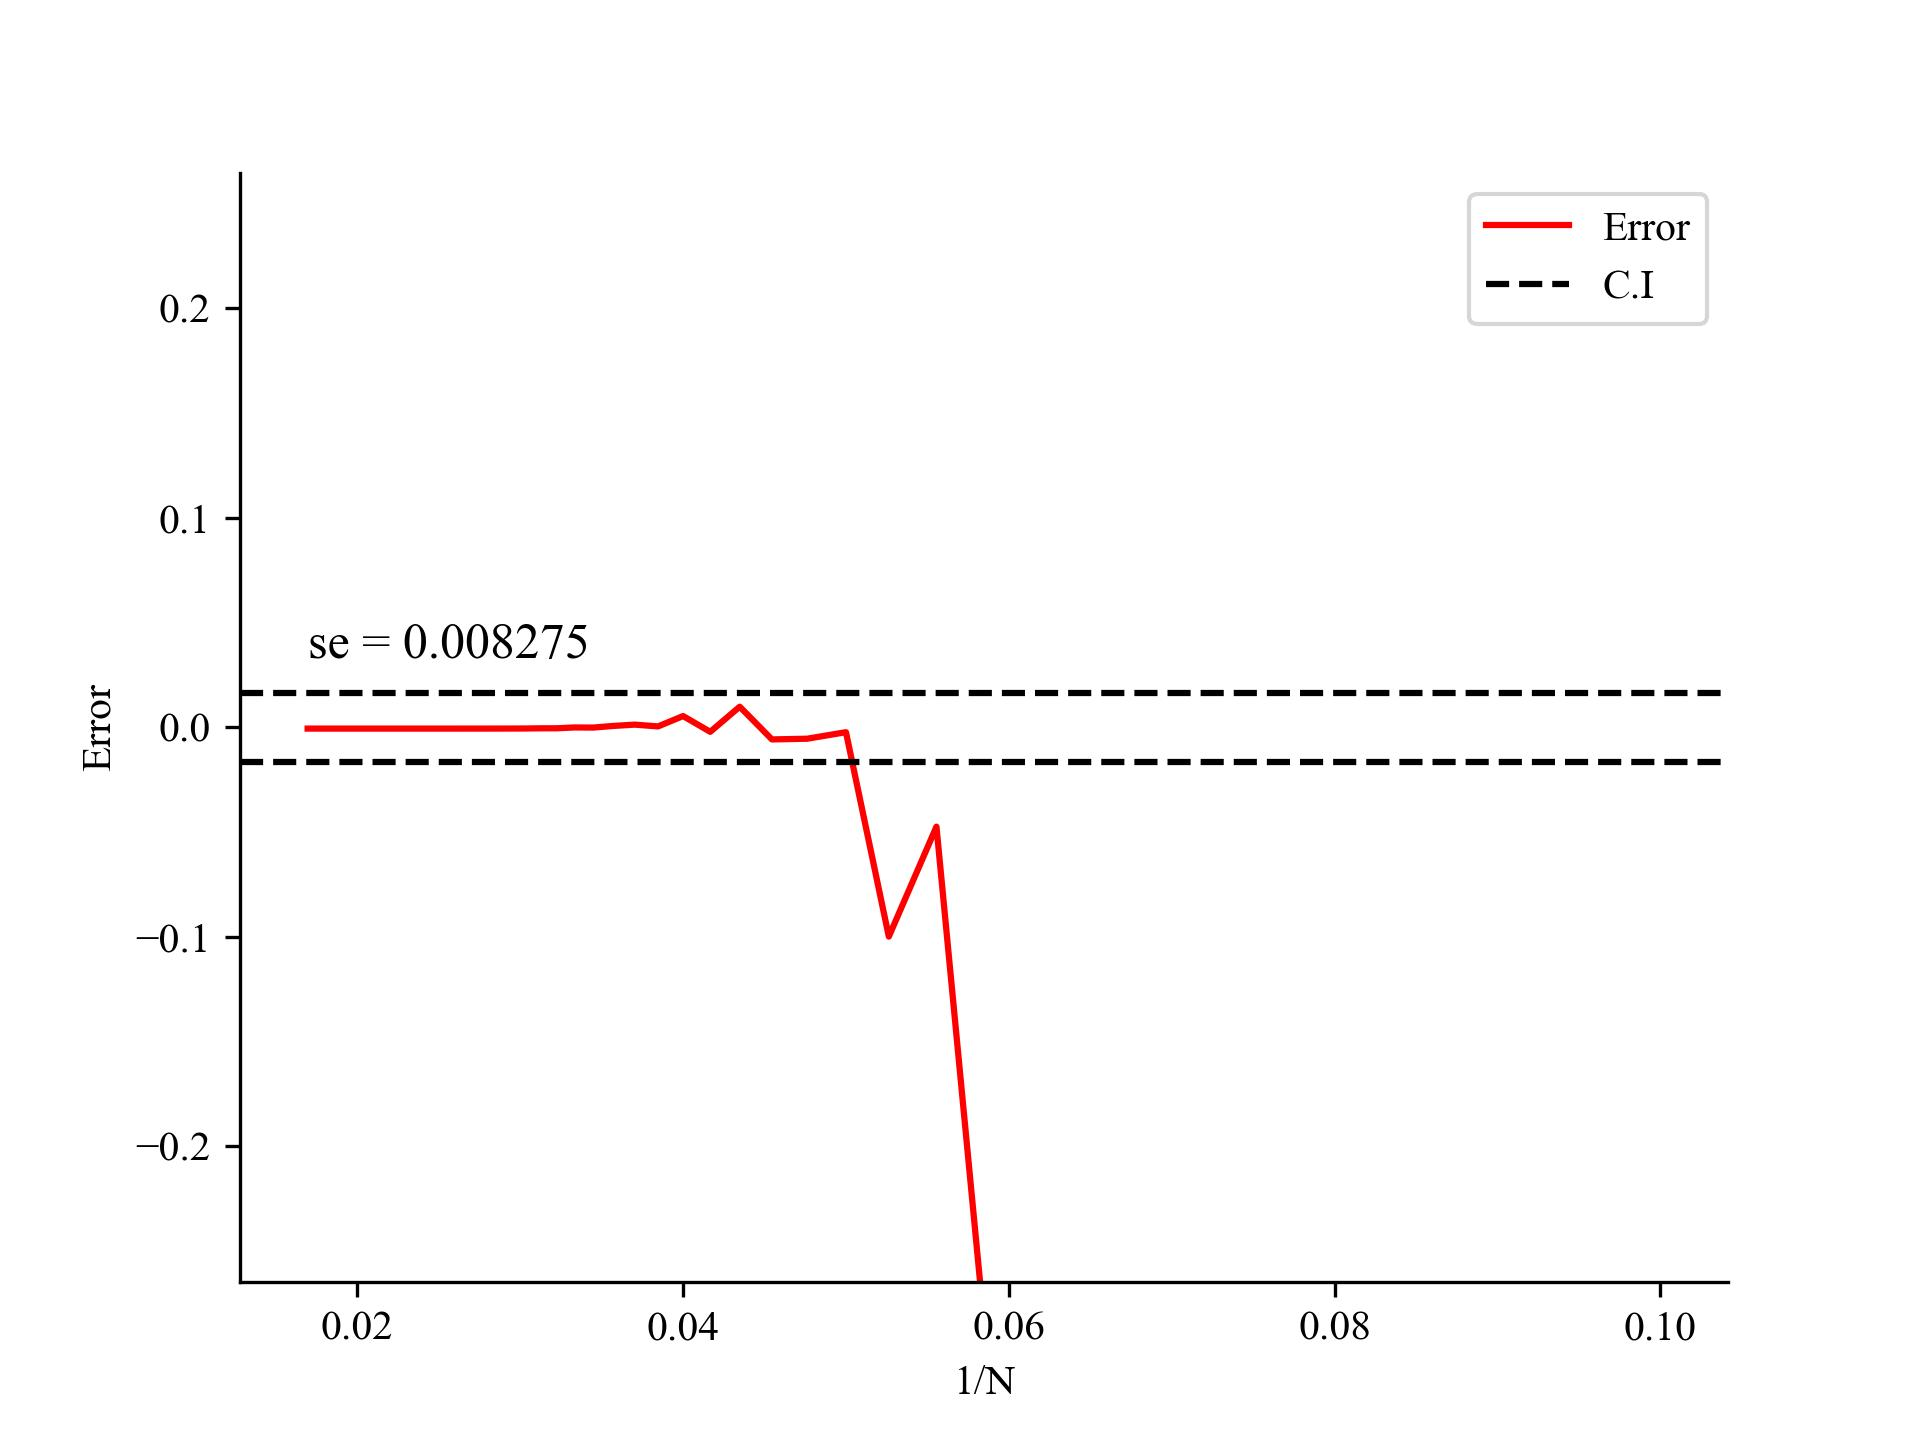
\includegraphics[width=0.8\linewidth]{value-plot-MJD-bothdown.jpg}
    \caption[\emph{JD-Down: Value accuracy comparing to the simulation with} $10^7$ \emph{paths.}]{\emph{JD-Down: Value accuracy comparing to the simulation with} $10^7$ \emph{paths.} \textbf{Note}: mean value from simulation = 33.154370, criteria of negligible error from the product of payoff function and density is $10^{-6}$, and $N$ starts from $10$  with increment $=2$.}

    \label{fig:label}
\end{figure}

\begin{figure}[H]
    \centering
    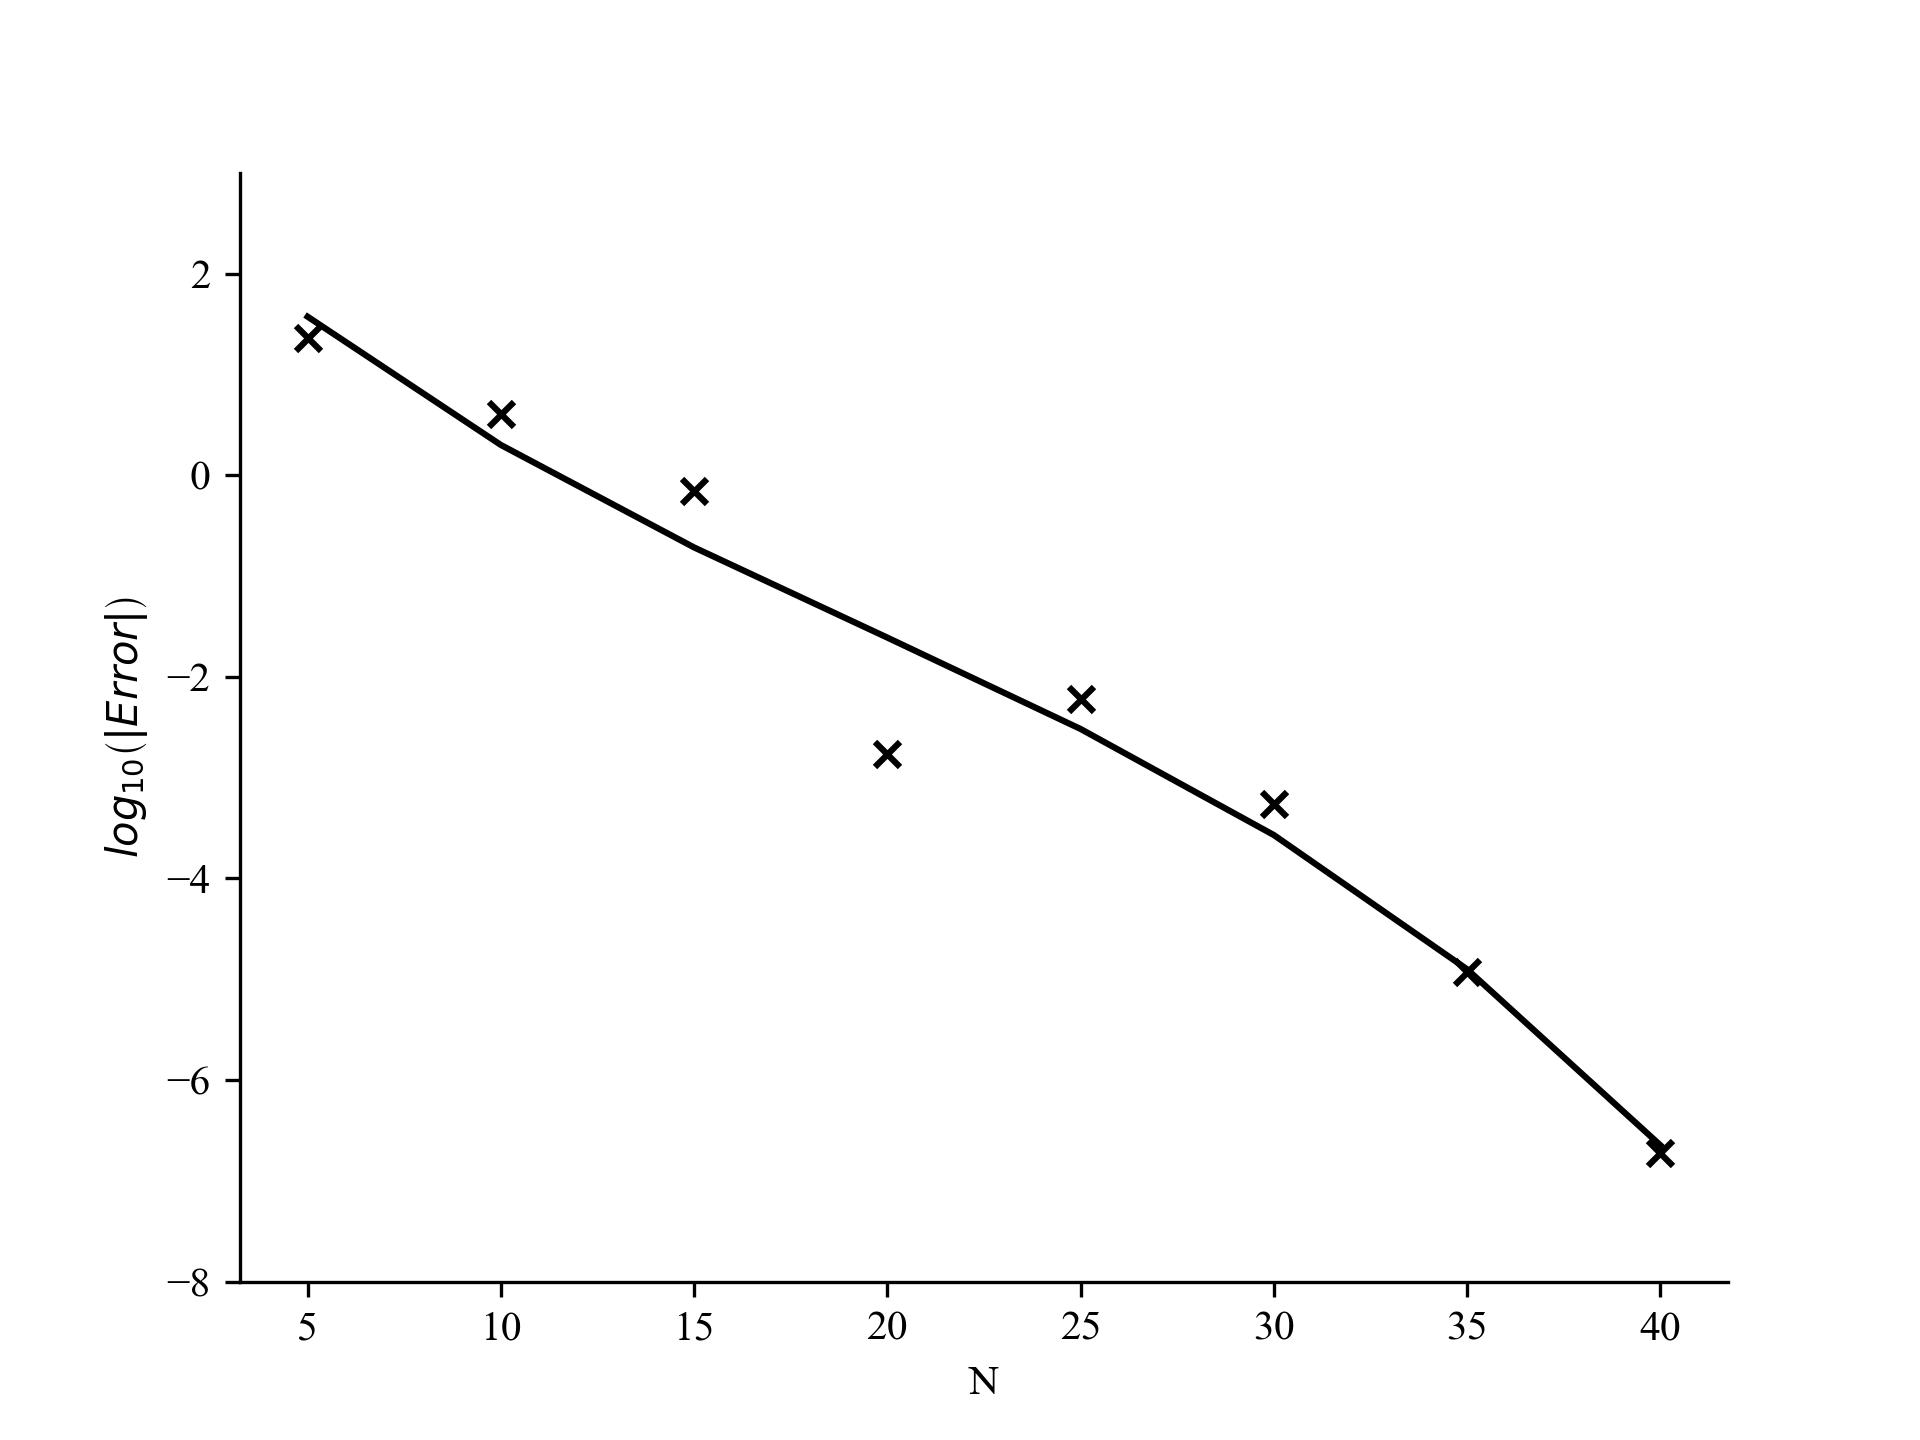
\includegraphics[width=0.8\linewidth]{error-plot-MJD-bothdown.jpg}
    \caption[\emph{JD-Down: The speed of error convergence.}]{\emph{DJD-Down: The speed of error convergence.} \textbf{Note}: reference value $=33.153704436$, criteria of negligible error from the product of payoff function and density is $10^{-15}$, $R^2=0.964$, and the regression line is $log_{10}\left(|Error|\right) = -0.0052N^2-0.0604N+1.5897$.}

    \label{fig:label}
\end{figure}


\subsection{Double Exponential Jump Diffusion Model}
\begin{figure}[H]
    \centering
    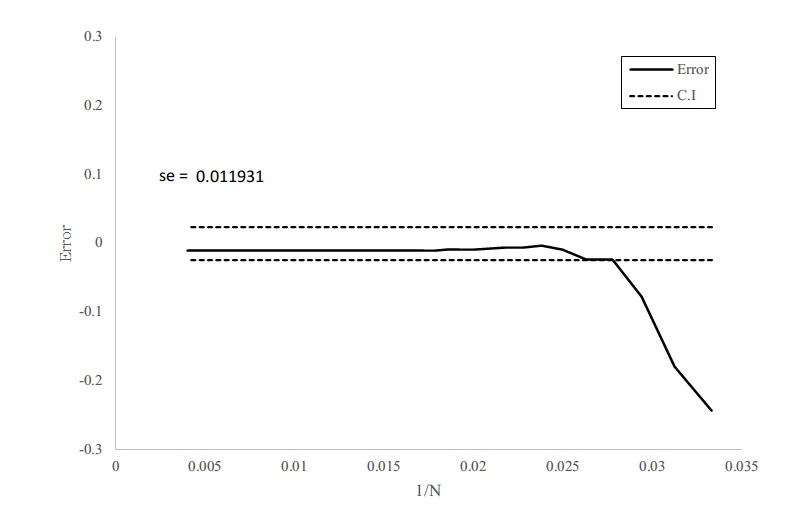
\includegraphics[width=0.8\linewidth]{value-plot-KJD-bothdown.jpg}
    \caption[\emph{DJD-Down: Value accuracy comparing to the simulation with} $10^7$ \emph{paths.}]{\emph{DJD-Down: Value accuracy comparing to the simulation with} $10^7$ \emph{paths.} \textbf{Note}: mean value from simulation = 43.817423, criteria of negligible error from the product of payoff function and density is $10^{-6}$, and $N$ starts from $10$  with increment $=2$.}

    \label{fig:label}
\end{figure}
\begin{figure}[H]
    \centering
    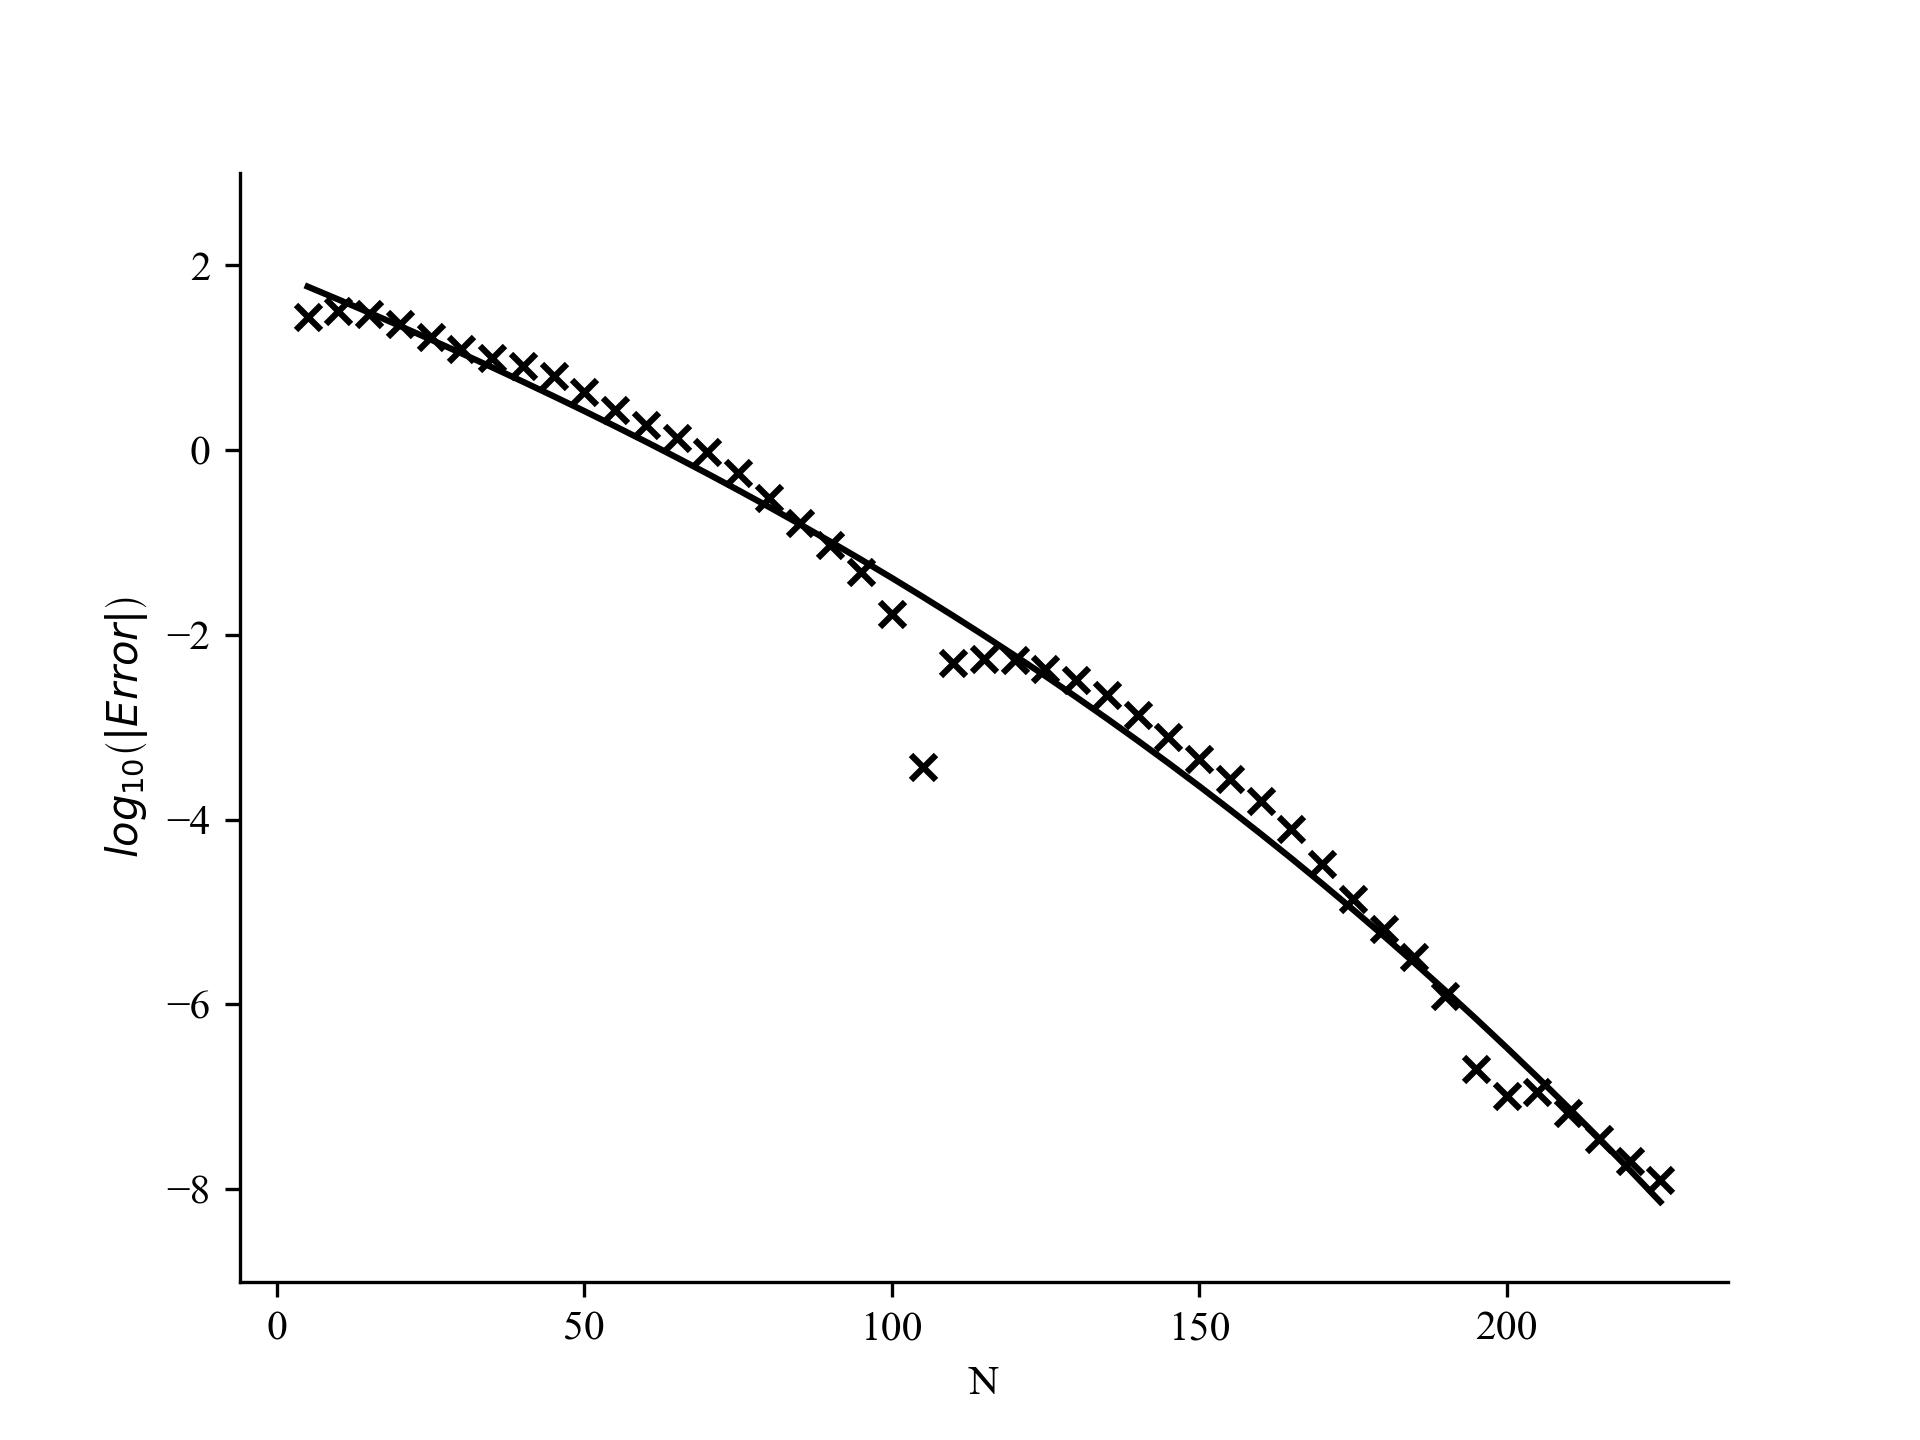
\includegraphics[width=0.8\linewidth]{error-plot-KJD-bothdown.jpg}
    \caption[\emph{DJD-Down: The speed of error convergence.}]{\emph{DJD-Down: The speed of error convergence.} \textbf{Note}: reference value $=43.8068018661$, criteria of negligible error from the product of payoff function and density is $10^{-15}$, $R^2=0.985$, and the regression line is $log_{10}\left(|Error|\right) = 1.039\times 10^{-5}N^2-0.0304N+1.9335$.}

    \label{fig:label}
\end{figure}



\subsection{Stochastic Volatility Jump Model}
\begin{figure}[H]
    \centering
    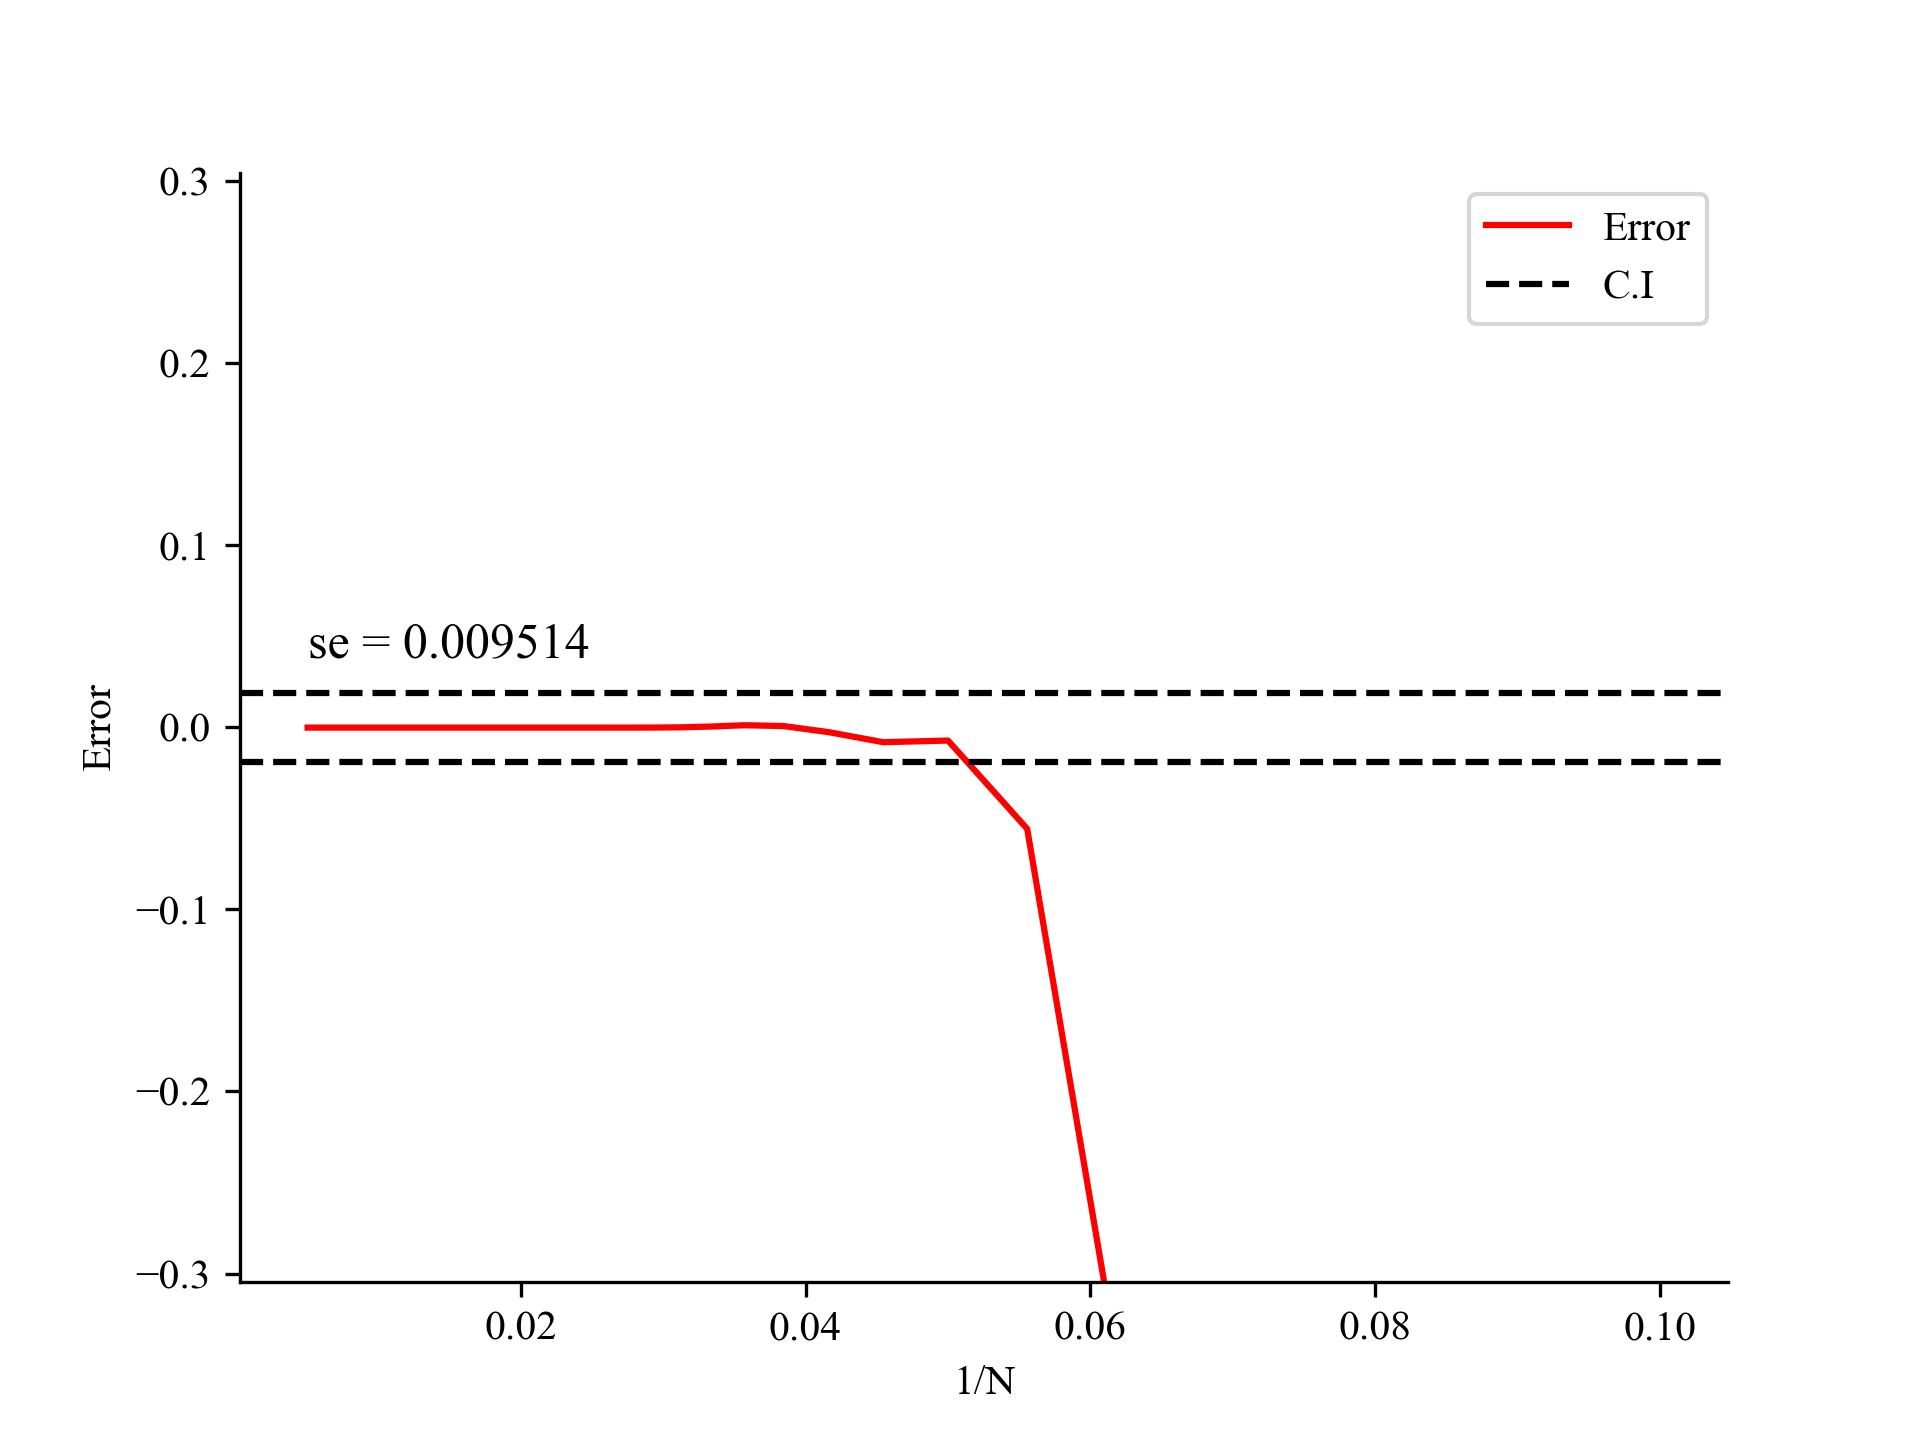
\includegraphics[width=0.8\linewidth]{value-plot-SVJ-bothdown.jpg}
    \caption[\emph{SVJ-Down: Value accuracy comparing to the simulation with} $10^7$ \emph{paths.}]{\emph{SVJ-Down: Value accuracy comparing to the simulation with} $10^7$ \emph{paths.} \textbf{Note}: the mean value from simulation = 33.197307, criteria of negligible error from the product of payoff function and density is $10^{-6}$, and $N$ starts from $10$  with increment $=2$.}

    \label{fig:label}
\end{figure}

\begin{figure}[H]
    \centering
    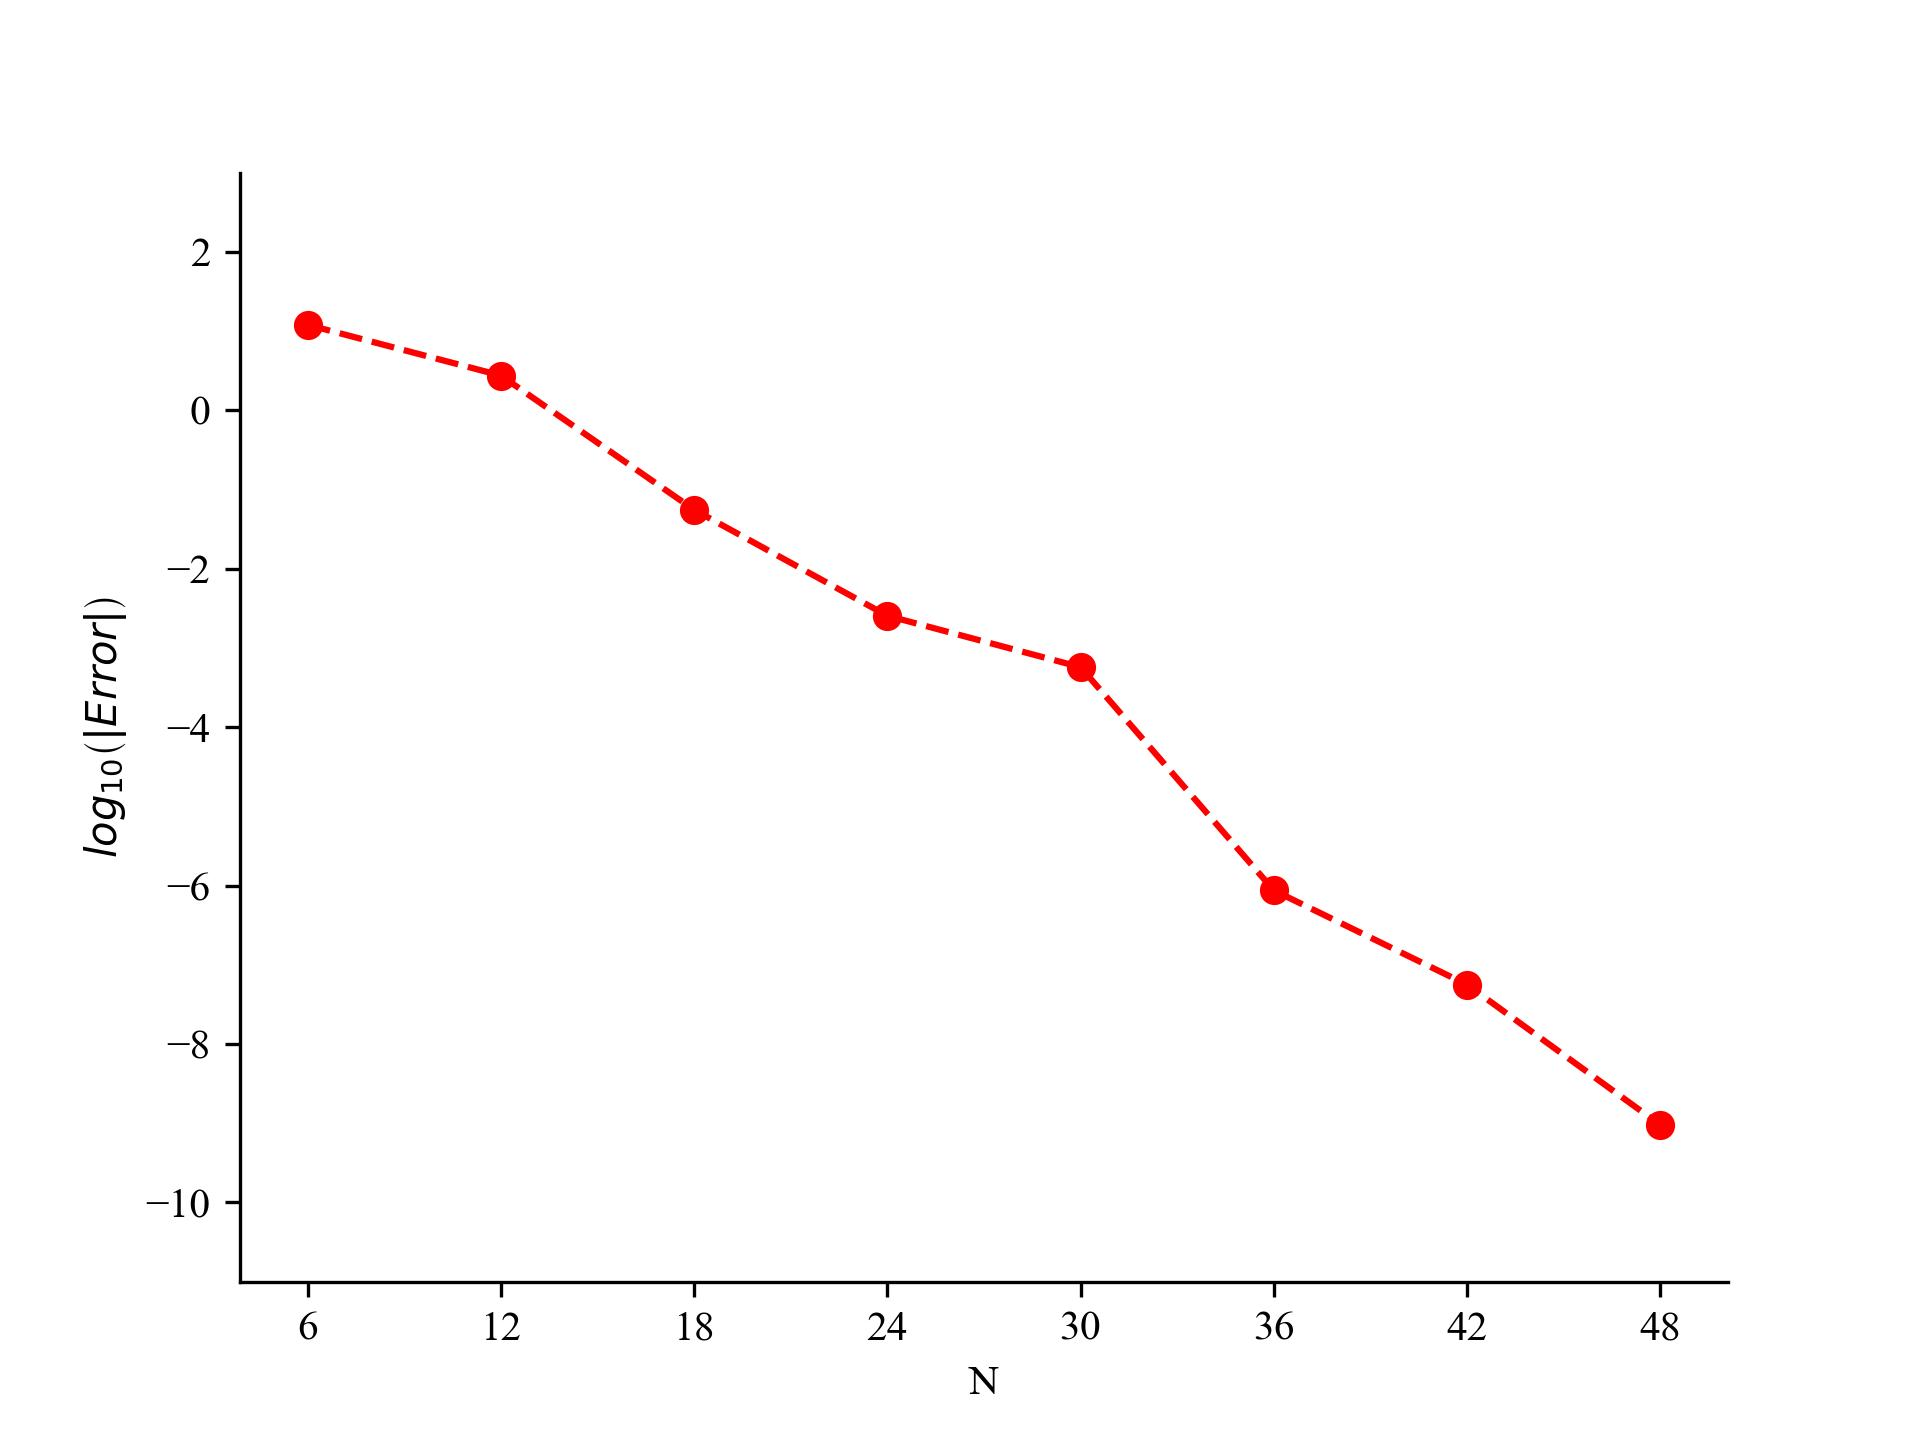
\includegraphics[width=0.8\linewidth]{error-plot-SVJ-bothdown.jpg}
    \caption[\emph{SVJ-Down: The speed of error convergence.}]{\emph{SVJ-Down: The speed of error convergence.} \textbf{Note}: reference value $=33.1970889218$, criteria of negligible error from the product of payoff function and density is $10^{-15}$, $R^2=0.985$, and the regression line is $log_{10}\left(|Error|\right) = -0.0052N^2-0.0058N+1.5678$.}

    \label{fig:label}
\end{figure}



\subsection{Normal Inverse Gaussian Model}
\begin{figure}[H]
    \centering
    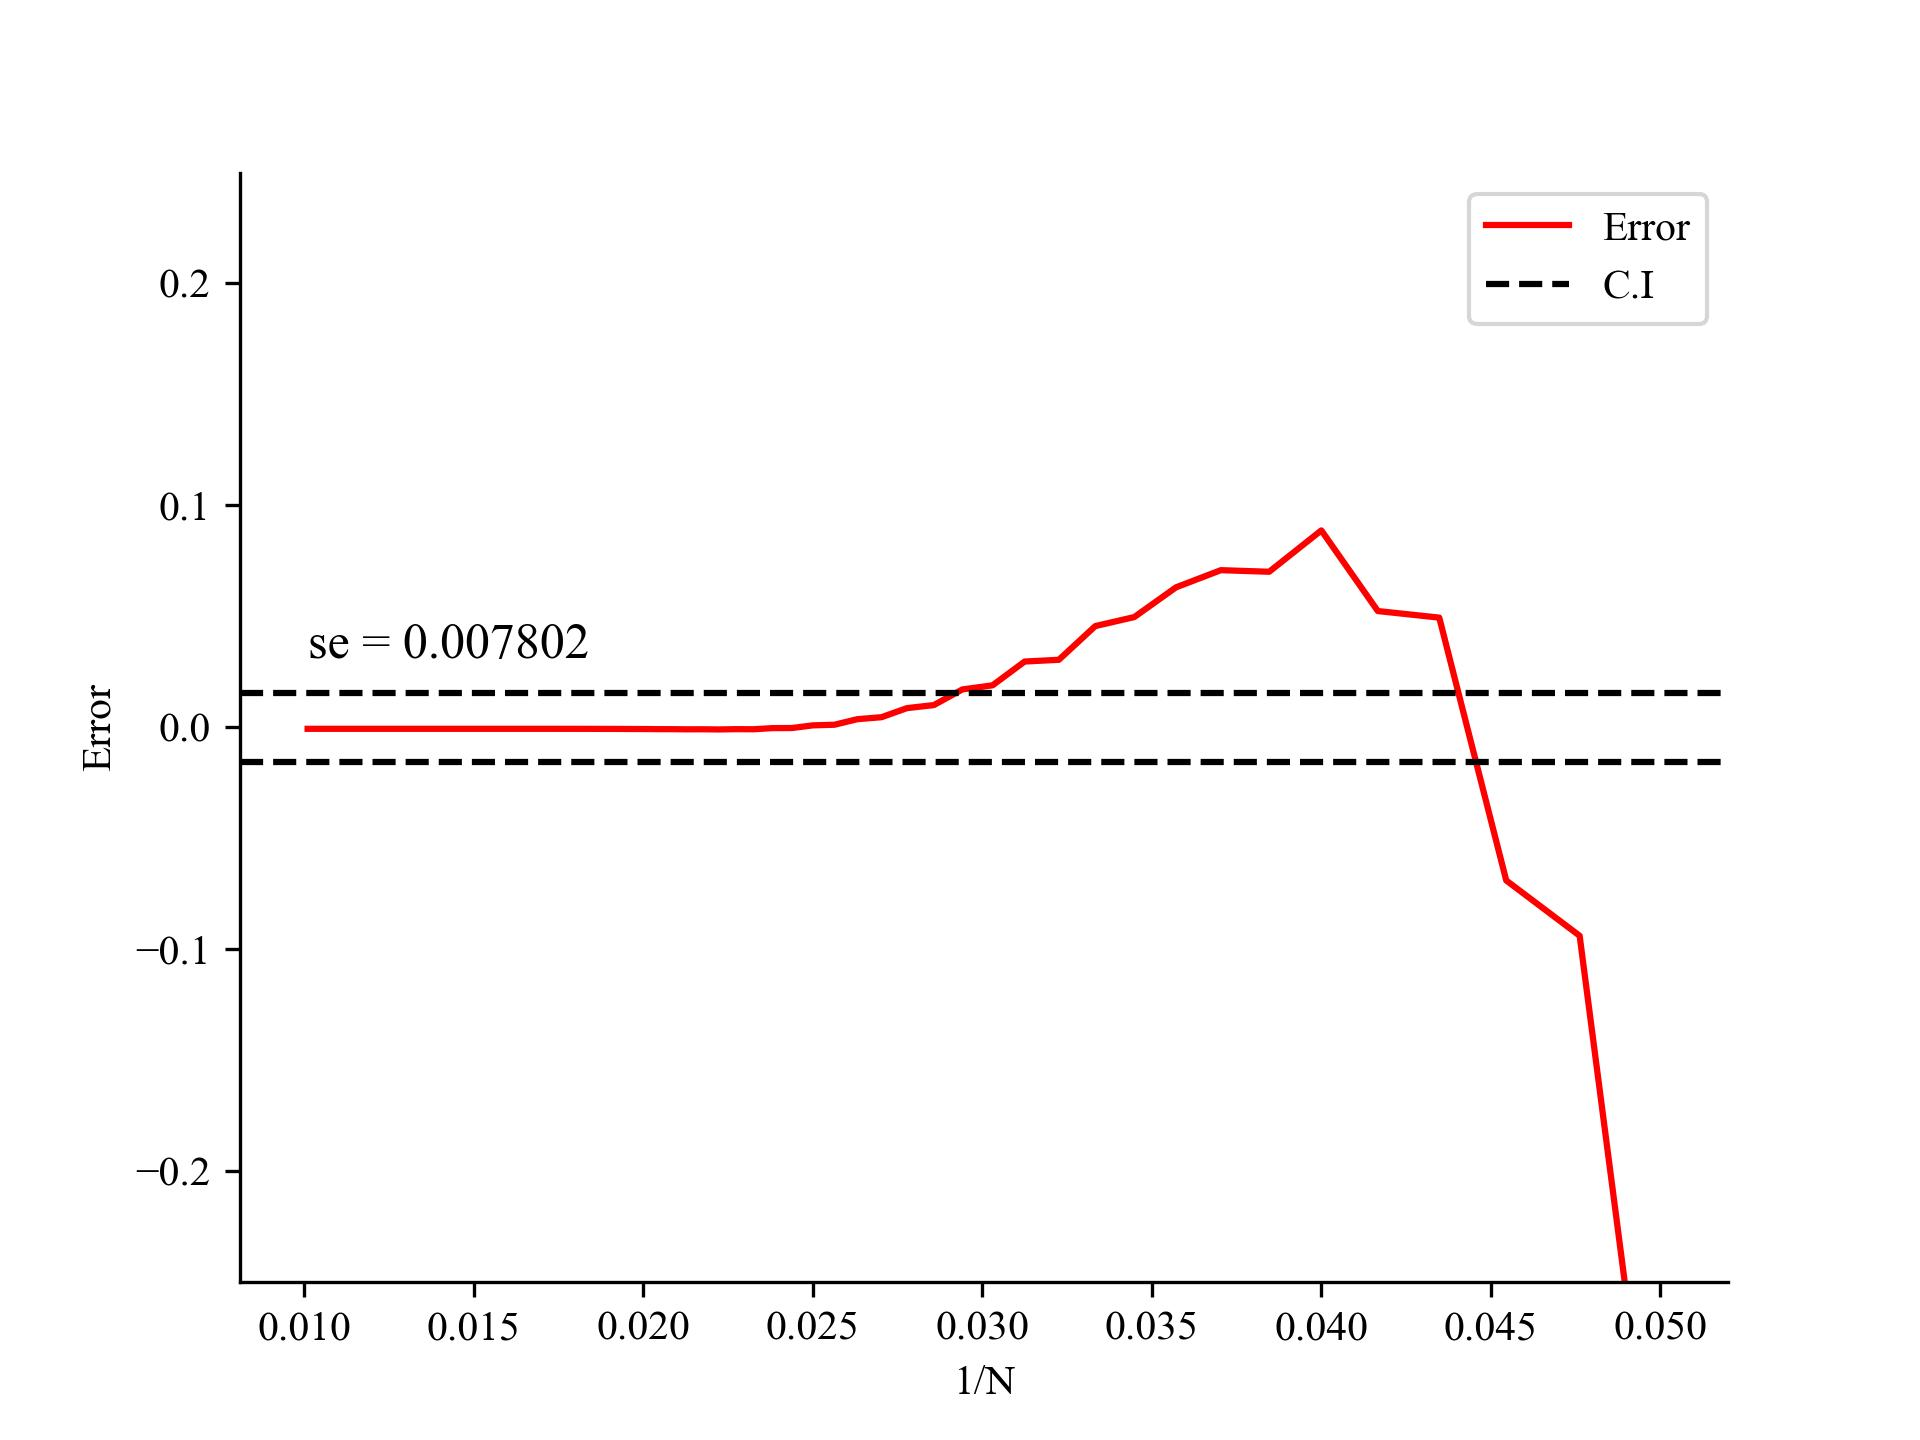
\includegraphics[width=0.8\linewidth]{value-plot-NIG-bothdown.jpg}
    \caption[\emph{NIG-Down: Value accuracy comparing to the simulation with} $10^7$ \emph{paths.}]{\emph{NIG-Down: Value accuracy comparing to the simulation with} $10^7$ \emph{paths.} \textbf{Note}: mean value from simulation = 35.340117, criteria of negligible error from the product of payoff function and density is $10^{-6}$, and $N$ starts from $10$  with increment $=2$.}

    \label{fig:label}
\end{figure}

\begin{figure}[H]
    \centering
    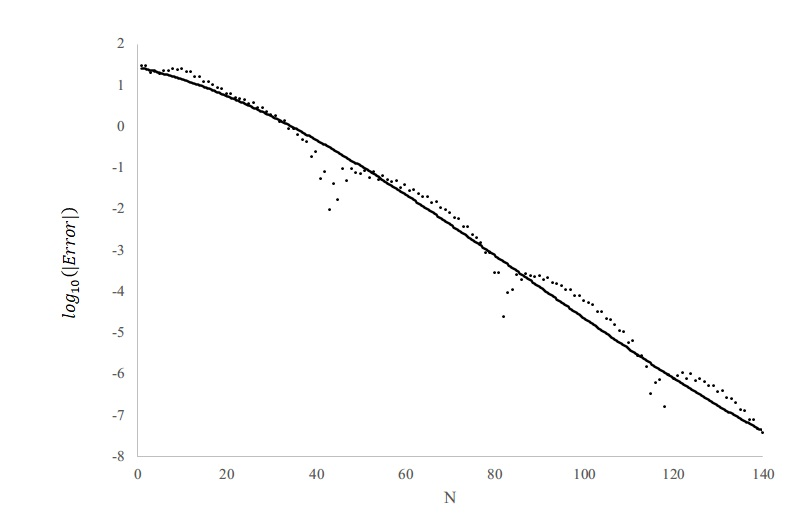
\includegraphics[width=0.8\linewidth]{error-plot-NIG-bothdown.jpg}
    \caption[\emph{NIG-Down: The speed of error convergence.}]{\emph{NIG-Down: The speed of error convergence.} \textbf{Note}: reference value $=35.3393903527$, criteria of negligible error from the product of payoff function and density is $10^{-15}$, $R^2=0.986$, and the regression line is $log_{10}\left(|Error|\right) = -0.0002N^2-0.0487N+1.7368$.}

    \label{fig:label}
\end{figure}


\subsection{Variance Gamma Model}
\begin{figure}[H]
    \centering
    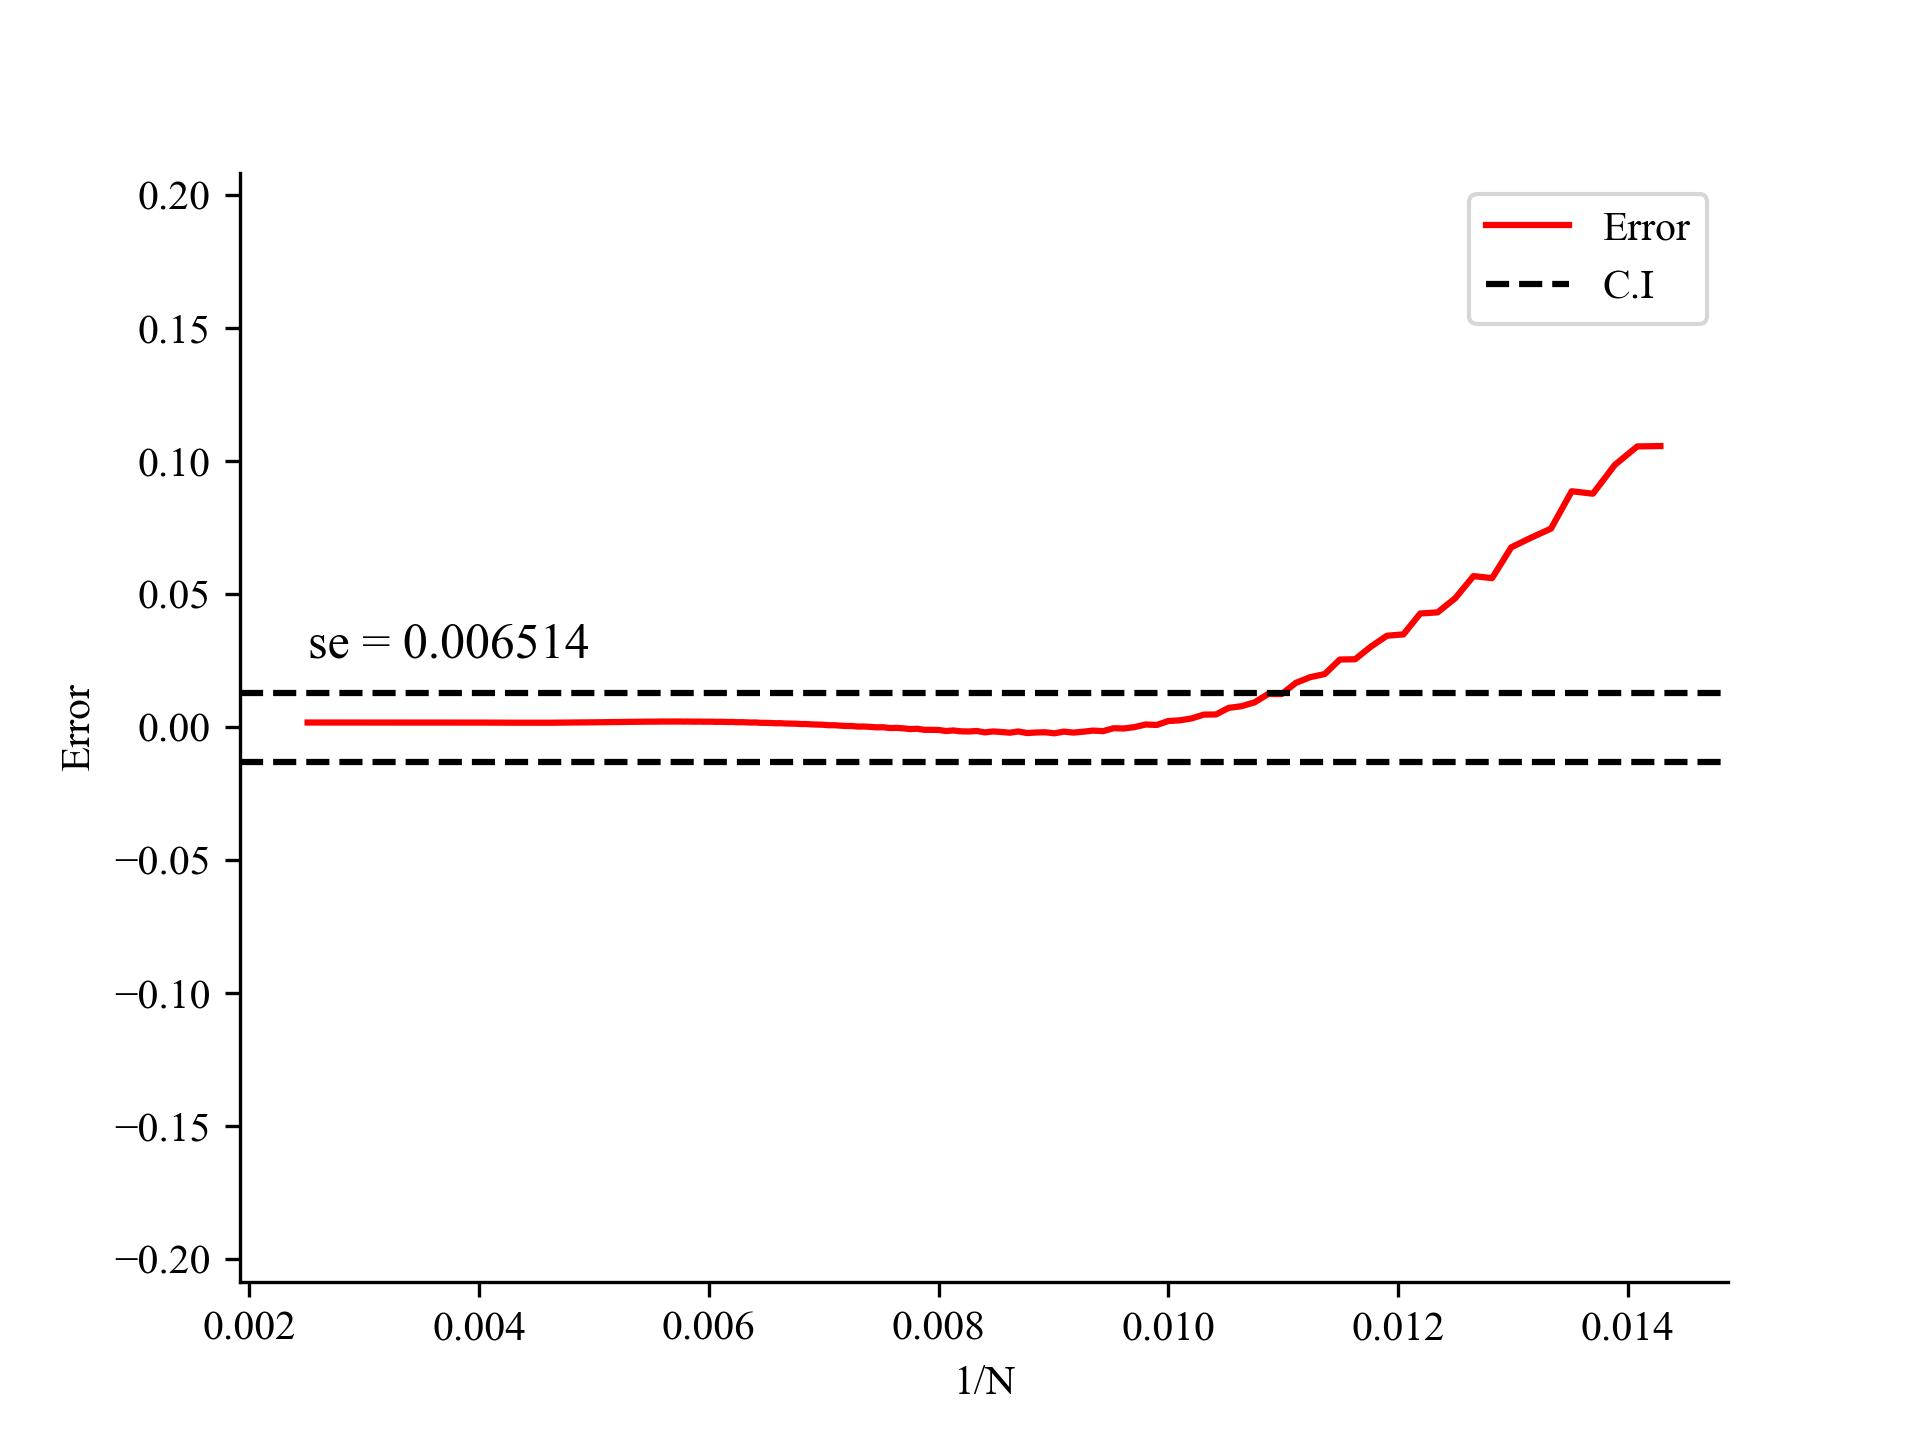
\includegraphics[width=0.8\linewidth]{value-plot-VG-bothdown.jpg}
    \caption[\emph{VG-Down: Value accuracy comparing to the simulation with} $10^7$ \emph{paths.}]{\emph{VG-Down: Value accuracy comparing to the simulation with} $10^7$ \emph{paths.} \textbf{Note}: mean value from simulation = 51.999204, criteria of negligible error from the product of payoff function and density is $10^{-6}$, and $N$ starts from $10$  with increment $=2$.}

    \label{fig:label}
\end{figure}

\begin{figure}[H]
    \centering
    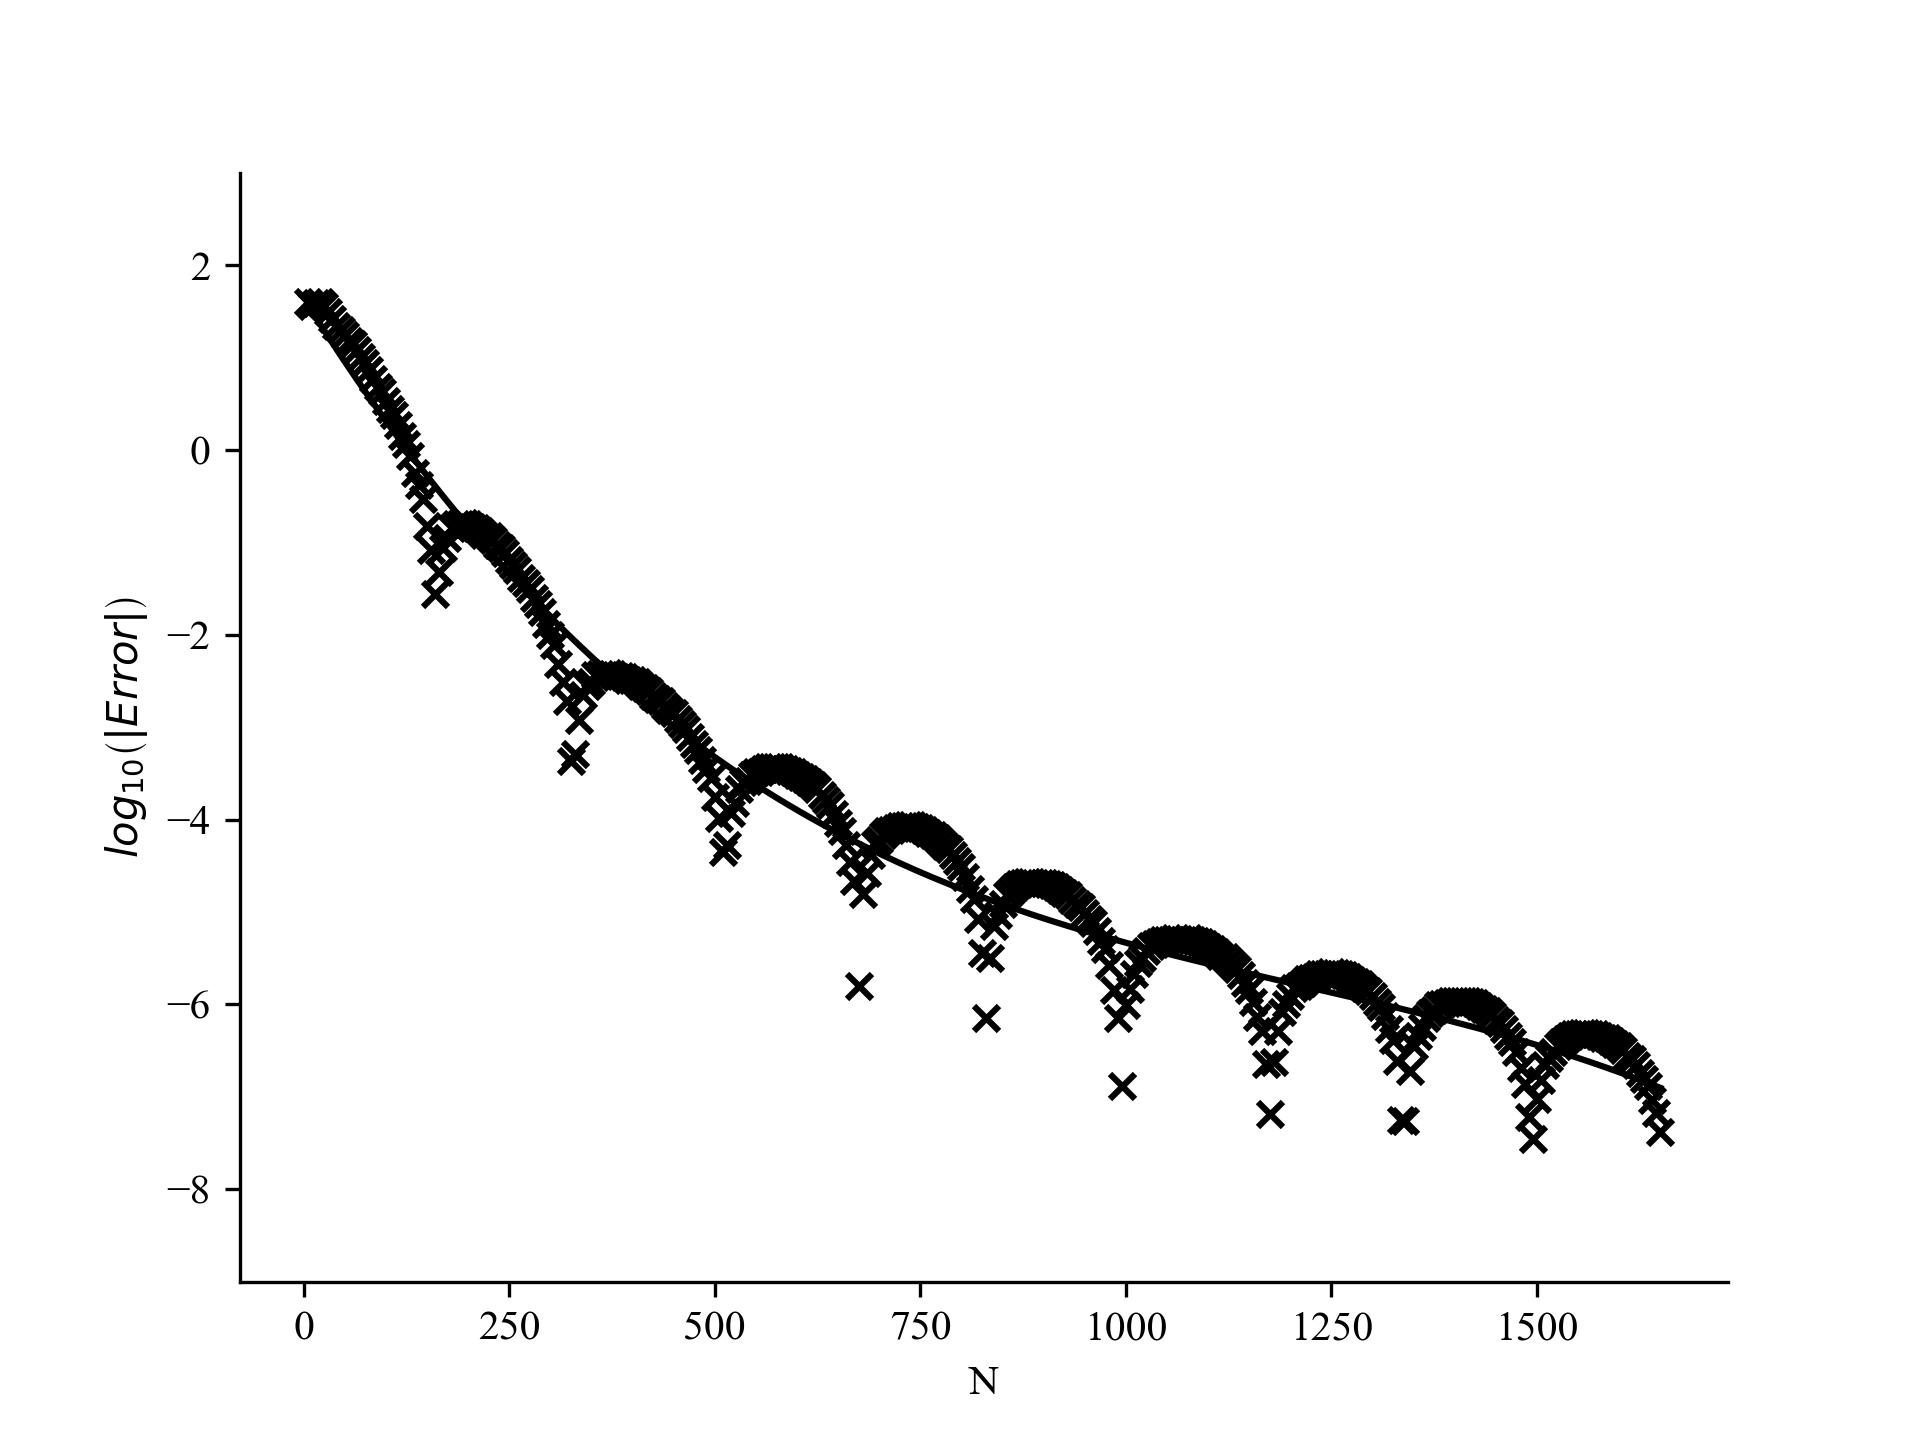
\includegraphics[width=0.8\linewidth]{error-plot-VG-bothdown.jpg}
    \caption[\emph{VG-Down: The speed of error convergence.}]{\emph{VG-Down: The speed of error convergence.} \textbf{Note}: reference value $=52.0009599216$, criteria of negligible error from the product of payoff function and density is $10^{-15}$, $R^2=0.972$, and the regression line is $log_{10}\left(|Error|\right) = 1.243\times 10^{-5}N^2-0.0173N+1.9176$.}

    \label{fig:label}
\end{figure}

\begin{figure}[ht]
    \begin{table}[H]
      \centering
      \caption[$log_{10}(|Error|)=AN^2+BN+C$]{Right Down - $log_{10}(|Error|)=AN^2+BN+C$}
    \end{table}
    \centering
        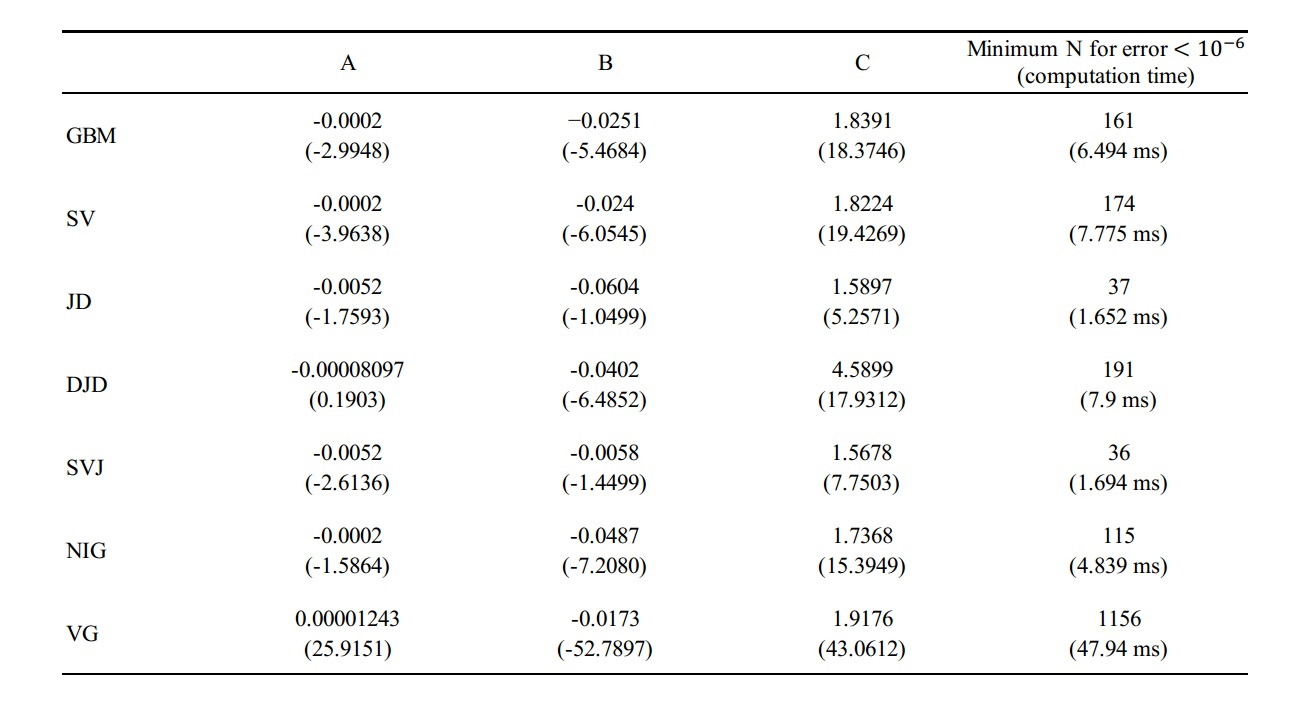
\includegraphics[width=1.1\textwidth,center]{bothdown-table.jpg}
    \caption*{\small{This table reports the coefficients of the regression and t-statistics shown inside the parentheses in accordance with the coefficient. The time measurements in the final column are expressed in milliseconds and pertain to the MacBook Air equipped with the Apple M1 chip.}}
\end{figure}

Under the concave payoff function for the right end, despite selecting a four-degree polynomial option, the highest degree term is larger than the call option and convex payoff for the right end in Table 3.2. However, compared to the convex payoff, it requires much fewer $N$. This is because, due to the property of the concave payoff function for the right end, the product of the payoff function and density function is zero on the far right. Therefore, there is no need to simulate over such a large range. As the interval between $l$ and $u$ increases, a larger $N$ is required for fitting. Furthermore, it also performs very well in terms of computation time, with a maximum time of only 0.0078 milliseconds to complete.


\section{Problem for Pricing Stochastic Double-Jump Stochastic Volatility Model}
The stochastic double jumps model is a widely recognized and valuable pricing model in the field of financial engineering. This stochastic process differs from other stochastic processes in that it incorporates jumps in both the variance and the rate of return simultaneously. However, during my attempts to apply this model for pricing purposes, we encountered an issue. Initially, I employed both simulation methods and numerical integration methods to price this stochastic process, and the results were consistent. However, when using my pricing approach, I discovered there is a division by zero error in computation. A singular point exists in the pricing process. To address this problem, let's provide a brief introduction to this stochastic process. Based on Duffie, Pan, and Singleton (2000) research, the process can be depicted by
\begin{align*}
d\left(\begin{array}{c}
Y_t \\
V_t
\end{array}\right)=\left(\begin{array}{c}
r-d-\lambda \mu-\frac{1}{2} V_t \\
\kappa_v\left(\bar{v}-V_t\right)
\end{array}\right) d t+\sqrt{V_t}\left(\begin{array}{cc}
1 & 0 \\
\bar{\rho} \sigma_v & \sqrt{1-\bar{\rho}^2} \sigma_v
\end{array}\right) d W_t^Q+d N_t,
\end{align*}
where $Y = \mathrm{ln}\left(S\right)$, $V$ is variance, $Z_t$ is a pure jump process in $\mathbb{R}^2$. The intensity of simultaneous correlated jumps in $Y$ and $V$ is $\lambda$. The distribution of the jump size in $V$ is exponential with mean $\mu_{c_v}$. The realization of jump size in $V$ is $z_v$. The jump size in $Y$ is a normal distribution with mean $mu_{c,y} + \rho_J z_v$ and variance $\sigma_{c,y}^2$. The characteristic function can be represented by
\begin{align*}
\varphi(v) & =\mathrm{exp}(\bar{\alpha} + \bar{\beta} \cdot V_0),
\end{align*}
where
\begin{align*}
\bar{\alpha} &= \alpha_0 + \lambda T \left(1 + \mu iv \right) + \lambda f, \\
\bar{\beta} &= -\frac{a\left(1 - \mathrm{e}^{-\gamma T}\right)}{2\gamma - \left(\gamma + b\right)\left(1 - \mathrm{e}^{-\gamma T}\right)},\\
\end{align*}
\begin{align*}
\alpha_0 &= -rT + \left(r - d\right)i v T, \\
&-k_v\bar{v}\left(\frac{\gamma + b}{\sigma_v^2}T +\frac{2}{\sigma_v^2}\mathrm{ln}\left[1-\frac{\gamma+b}{2\gamma}\left(1-\mathrm{e}^{-\gamma T}\right)\right]\right),\\
f &= \mathrm{exp}\left(\mu_{c,y} i v+\sigma_{c,y}^2\frac{v^2}{2}\right)\zeta, \\
a &= iv\left(1-iv\right),\\ 
b &= \sigma_v \bar{\rho} iv - k_v,\\
c &= 1 - \rho_J\mu_c^v u,\\ 
\gamma &= \sqrt{b^2 + a \sigma_v^2},\\ 
\mu &=\frac{\exp \left(\frac{1}{2} \sigma_{c, y}^2\right)}{1-\rho_J \mu_{c, v}},
\end{align*}
and
\begin{align}
\zeta &= \frac{\gamma-b}{(\gamma-b) c+\mu_{c, v} a} \tau \nonumber \\
&-\frac{2 \mu_{c, v} a}{(\gamma c)^2-\left(b c-\mu_{c, v} a\right)^2} \ln \left[1-\frac{(\gamma+b) c- \mu_{c, v} a}{2 \gamma c}\left(1-e^{-\gamma \tau}\right)\right]. \label{SVJJ problem}
\end{align}

When using this pricing formula, it is necessary to substitute $v=0$ into the characteristic function when calculating the first term of summation. However, this may cause problems. The denominator of the second part of $(\ref{SVJJ problem})$,
$$(\gamma c)^2-\left(b c-\mu_{c, v} a\right)^2 = 0,$$
where $\left(\gamma c\right)=bc$ and $\left(bc - \mu_{c,v}a\right)=bc$ because of $a=0$. It can be observed that this will result in the point being undefined in the complex space. Firstly, I attempted to replace $v=0$ with a very small number as a proxy for the limit in this method, but the results did not show significant changes. This value did not align with the results obtained from either the numerical integration method or the simulation method which deviates significantly from the confidence interval. In addition, I used the property of the characteristic function referencing Bakshi and Madan (2000), which says the value of the characteristic function equals 1 when $v=0$. However, this attempt did not alter the pricing results compared to using the first attempt of replacing with a limit proxy. I reviewed past research and found that, in most cases, the singularity position is replaced with a very small value or avoided by this point through numerical integration. Although some approaches are based on the Fourier method which is based on numerical integration, the methodologies are different from my method which is based on the Fourier expansion of density function. I believe that numerical integration methods are generally unaffected by the presence of singularities in the characteristic function, as long as these singular points are carefully avoided during the integration calculation. However, my method employed in the research necessitates a characteristic function free of singular points to accurately approximate the entire density function.\\
